\documentclass[10pt]{article}

\usepackage{amssymb,amsfonts,amsmath,amsthm}
\usepackage{algorithm,algpseudocode}
\usepackage{enumitem}
\usepackage{graphicx}
\usepackage{mathtools}
\usepackage{multicol,multirow,fullpage}
\usepackage{url}
\usepackage{subfigure}
\usepackage{listings}
\usepackage{xltxtra,fontspec,xunicode}
\usepackage{longtable}
\defaultfontfeatures{Scale=MatchLowercase}
\setmonofont{VTScreenplayUnderwoodB}

\DeclarePairedDelimiter\abs{\lvert}{\rvert}
\DeclarePairedDelimiter\norm{\lVert}{\rVert}
\DeclarePairedDelimiter\parens{(}{)}
\DeclarePairedDelimiter\curly{\{}{\}}
\DeclarePairedDelimiter\ceil{\lceil}{\rceil}
\DeclarePairedDelimiter\floor{\lfloor}{\rfloor}

%% star versus non-star.
\makeatletter
 \let\oldabs\abs
 \def\abs{\@ifstar{\oldabs}{\oldabs*}}
 \let\oldnorm\norm
 \def\norm{\@ifstar{\oldnorm}{\oldnorm*}}
 \let\oldparens\parens
 \def\parens{\@ifstar{\oldparens}{\oldparens*}}
\makeatother

\algnewcommand{\LineComment}[1]{\State \(\triangleright\) #1}

\newcommand{\suchthat}{\, \mid \,}
\newcommand{\bigO}[1]{\mathcal{O}{\parens{#1}}}
\newcommand{\bigOmega}[1]{\Omega{\parens{#1}}}
\newcommand{\bigTheta}[1]{\Theta{\parens{#1}}}
\newcommand{\littleO}[1]{o{\parens{#1}}}
\newcommand{\littleOmega}[1]{\omega{\parens{#1}}}

\newcommand{\kmax}{k_{\max}}
\newcommand{\logkmax}{\log_{2}{\kmax}}
\newcommand{\topk}[2]{\mathrm{top}_{#1}\parens{#2}}
\newcommand{\topkmax}[1]{\topk{\kmax}{#1}}
\newcommand{\dataset}{\curly{f_{i}}}
\newcommand{\bigassexpression}{\bigO{ \frac{N}{B}\alpha \parens{\frac{N}{B}} \parens{\sqrt{\log{\frac{N}{B}}} + \log{\frac{\kmax}{B}}}} }

\newcommand{\listj}{\texttt{list}_{j}}
\newcommand{\tmplist}{\texttt{list}}
\newcommand{\tmptopk}{\texttt{topk}}
\newcommand{\tree}{\texttt{tree}_{j}}
\newcommand{\key}{\texttt{key}}
\newcommand{\val}{\texttt{value}}

\newcommand{\na}{\textit{n/a}}
\newcommand{\ditto}{\textit{do.}}


\newtheorem{lemma}{Lemma}

\hyphenation{Geo-Wave}
\hyphenation{Geo-Mesa}
\hyphenation{Geo-Trellis}
\hyphenation{Simple-Feature}
\hyphenation{Simple-Feature-Type}

\begin{document}

\title{GeoMesa and GeoWave Comparative Analysis: Final Report}

\author{Azavea, Inc.}

\date{}

\maketitle

\begin{abstract}
  This document details the results of a comparative analysis between two open source geospatial big data frameworks: GeoWave and GeoMesa.
  A feature comparison and a set of performance tests with analysis are presented.
  We have concluded that despite a large set of overlapping features, specifically the capability to index and query spatial and spatiotemporal data in Accumulo, the projects differ from each other in substantial ways.
  Through analyzing performance test data, we make four conclusions about the performance characteristics of the current versions of the systems - GeoMesa 1.2.6 and GeoWave 0.9.3 - for the use case of indexing spatial and spatiotemporal data in Accumulo: (1) GeoMesa performed better against queries with large result counts - i.e. queries that were not highly selective - while GeoWave performed better on smaller result sets - i.e. queries that selected fewer results out of a larger dataset; (2) GeoWave performed better against queries with larger temporal bounds, while GeoMesa performed better when the temporal bounds were smaller (around a couple of weeks or less); (3) GeoMesa performed better in the non-point dataset use case; and (4) GeoWave outperformed GeoMesa in multitenancy use cases, where there are 16 to 32 queries being executed against the system in parallel.
  We also find the two systems perform reasonably well in all cases, and that neither system was dominant in performance characteristics.
  We conclude by providing recommendations for ways the two projects can collaborate moving forward in light of this analysis.
\end{abstract}

\section{Introduction}
\label{sec:introduction}

GeoMesa and GeoWave are two open source projects that deal with large geospatial data.
At a high level, these projects offer solutions to many of the same types of problems.
Because of this overlap, it has been difficult for new users approaching the big geospatial data community to understand what the differences are between these projects and what project should be used under what circumstances.
For some of their most overlapping functionality, for example, indexing spatial and spatiotemporal data in Accumulo, the differences between the two projects can be unclear even to veterans of big geospatial data processing.
This document aims to address this lack of clarity by discussing the many significant differences between the projects;
differences in form, function, and performance.

In the summer of 2016, Azavea conducted a comparative analysis of GeoWave and GeoMesa in order to gain a deeper understanding of the two projects and to share that understanding with the geospatial big data community.
This document contains the results of our efforts and aims to provide a more clear picture of how the projects are different from each other and what use cases fit best to either project.
We hope this will aid the geospatial big data community in gaining a deeper understanding of these two outstanding projects and allow a better utilization of their functionality.

Along with an understanding how the projects are different from each other, this comparative analysis aims to provide information and guidance to potential future collaboration efforts between the GeoWave and GeoMesa projects.

This document assumes prior knowledge about the GeoMesa and GeoWave projects and is not intended to be an introduction to those projects.
For background information, please see the project websites:


\begin{itemize}
\item  GeoWave: \url{http://ngageoint.github.io/geowave/}
\item  GeoMesa: \url{http://www.geomesa.org/}
\end{itemize}

\section{Feature Comparison}
\label{sec:featurecompare}

The GeoMesa and GeoWave projects contain many features that overlap, and many that do not.
The Venn diagram shown in Figure \ref{venn} is not a complete list of features,
but indicates the significant overlap of the core features of GeoWave and GeoMesa and some of the distinguishing features that set them apart.

\begin{figure}[h!tb]
  \centering
  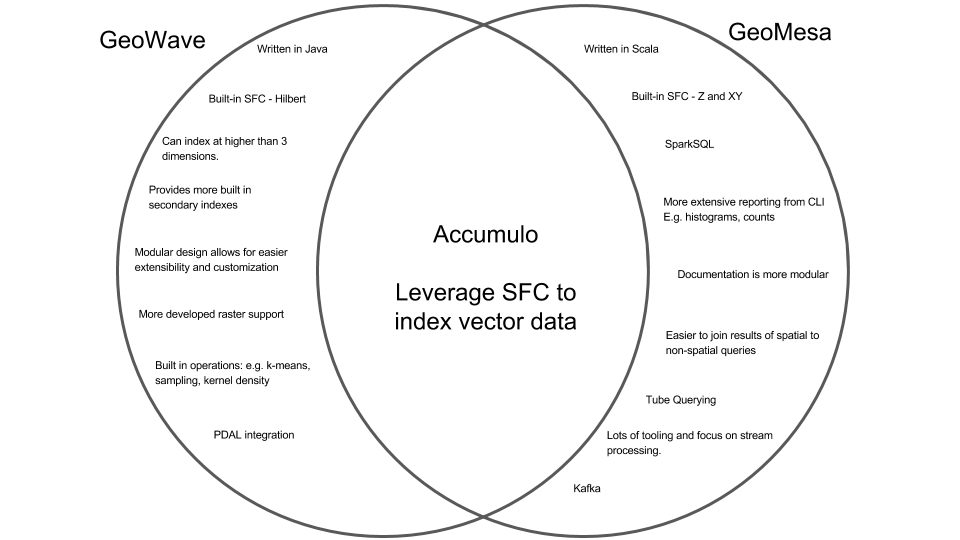
\includegraphics[width=0.60\textwidth]{../docs/img/venn-diagram.png}
  \caption{Venn Diagram of features.}
  \label{venn}
\end{figure}

As is illustrated in the diagram, there is a major overlap when it comes to a core feature of the two projects, namely using space filling curves to index geospatial data in Accumulo.
However, there are many features that differentiate the projects from one another.
Below is a summary table of feature similarities and differences.
A more detailed list of features can be found in Appendix \ref{appendix:features}: Details of GeoMesa and GeoWave features.

\subsection{Generality of the Architecture}
\label{sec:featurecompare:generality}

A major difference between the projects is the generality of the architectures when it comes to supporting
various backends\footnote{Backend refers to the specific mechanism for storing vector, data and the related geospatial index (ex: Accumulo, HBase).}
and indexing strategies.
GeoWave API has a focus on being an N-Dimensional indexing mechanism for arbitrary backends.
The fact that this document focuses on its ability to handle geospatial data ($2$-Dimensional spatial and $3$-Dimensional spatiotemporal data) is only based on the currently known GeoWave use cases.
However, the project aims at supporting data with arbitrary dimensionality.
GeoMesa API, on other hand, is directly tailored to geospatial indexing allowing for clearer interface, implementation, and paths for optimization.

GeoWave specifically is designed around abstractions that remain agnostic about the storage and access implementations.
This could provide more flexibility for developing backend support, which might explain why GeoWave HBase support is more mature than GeoMesa's.
GeoMesa focuses on using GeoTools' abstractions, and thus is more dependent on GeoTools as a base library.
GeoMesa also focuses less on dealing with abstractions; this may have an effect that features written for one backend are difficult to translate to another backend.
However, dealing with less abstraction can be more straightforward, and some developers may find it easier to understand and work with the GeoMesa API.

\section{Language}
\label{sec:featurecompare:language}

GeoMesa is developed using Scala, and GeoWave is developed using Java.
Both Scala and Java are languages in which the source compiles down to Java Virtual Machine (JVM) bytecode, which is executed on top of the same JVM.
This means that both projects can use the same dependencies, as can be observed by each project's reliance on GeoTools (a Java based geospatial library) for some of its features, including a core data type: the GeoTools \texttt{SimpleFeature}.
However, the differences between the Scala and Java languages are many, and it remains one of the biggest differences between the projects.

%% And user familiarity with the implementation languages should be considered as factor.
%% We will address this from the perspective of Java developers as they are a larger group of potential users.
%% GeoWave uses standard and well structured Java composition and design patterns both in its API and implementation and should provide few surprises for Java developers.
%% GeoMesa, though written in Scala, implements a GeoTools API that allows Java developers to easily use GeoMesa functionality without having to write Scala.
%% Java interoperability is a core design concern in GeoMesa API as evidenced by tutorial code being provided exclusively in Java.
%% This has limits, however, as developers investigating stack traces and exploring the GeoMesa implementation will encounter Scala.
%% Being Scala developers we can comment that GeoMesa codebase uses direct dialect of Scala, eschewing advanced language features and staying close to Java patterns which optimizes its readability for such a developer.
%% Ultimately the feasibility of this should be part of individual team evaluation when adopting either project.

\subsection{Accumulo Indexing}
\label{sec:featurecompare:indexing}

The two projects approach indexing in Accumulo in a similar way, but there are some key differences.

\subsubsection{Choice of Space Filling Curve}
\label{sec:featurecompare:indexing:curve}

GeoMesa supports the space filling curve indices named Z-order and XZ indices, while GeoWave supports Hilbert curves.
These space filling curve implementations have different properties that affect performance, such as the number of false positives returned and number of duplicate entries to be indexed.
You can read more about the differences in performance characteristics in Appendix \ref{appendix:planning}: Details of Performance Test Conclusions.

\subsubsection{Sharding}
\label{sec:featurecompare:indexing:sharding}

By default, GeoMesa uses ``sharding'', a technique of prefixing indices with a discrete number of shard IDs in order to better distribute the data across nodes of a cluster.
There is a trade-off between increasing distribution while decreasing locality.
Index sharding leads to more even per-query cluster resource utilization, which covers the common use cases GeoWave has the ability to shard, although in GeoWave it's called partitioning the data.
You can create a compound index with any of the GeoWave indexing strategies in order to partition.
Unlike GeoMesa, GeoWave partitioning is not enabled by default.
It is also configurable: you can decide on the number of partitions (i.e. shards) you want, and determine whether or not it's a round robin or hashing strategy that determines the partition ID.
GeoMesa's sharding seems to only use a hashing algorithm and a non-configurable number of shards.
In our benchmarks we had to enable index partitioning in GeoWave in order to improve its performance and make the benchmarks comparable.

\subsubsection{Periodicity}
\label{sec:featurecompare:indexing:periodicity}

To get around the problem of unbounded dimensions, such as time, the concept of ``periodicity'' is used in both GeoMesa and GeoWave.
This feature is similar to a shard, in that it prefixes an index with some ID.
A simple way to think of periodicity is that it bins each space filling curve into one period; for example, for one week.
In GeoWave, you can configure any dimension to have a periodicity of a configurable length.
With GeoMesa, you can configure the periodicity of the time dimension to day, week, month, or year.

\subsubsection{Tiered indexing vs XZ index}
\label{sec:featurecompare:indexing:versus}

GeoMesa uses an XZ index to handle non-point data, which allows the data to be stored at specific space filling curve resolutions based on the the size of the geometry.
GeoWave uses a technique called tiered indexing to handle this issue.
The technical differences between the two approaches are beyond the scope of this document.
Broadly, they have comparable theoretical performance with tiering being more flexible of the two, allowing for more use-case specific optimization.
However one major difference between the two approaches is that the XZ approach does not store any duplicates of data, while the tiered strategy can store up to four copies of an entry.

\subsection{Other features}
\label{sec:featurecompare:other}

This section gives a summary of features that are either found in one project and not the other,
or are found in both projects with considerable differences.


\subsubsection{Features Found in GeoWave and not in GeoMesa}
\label{sec:featurecompare:other:wave}

\begin{itemize}
\item Integration with Mapnik
\item Integration with PDAL for reading and writing point cloud data from/to GeoWave
\item Time interval queries: The ability to index data that exists within an interval of time, and query for intersecting intervals
\item Pixel-level subsampling: A visualization performance optimization that returns a subset of the resulting data based on pixel width
\item DBScan clustering
\end{itemize}


\subsubsection{Features Found in GeoMesa and not in GeoWave}
\label{sec:featurecompare:other:mesa}

\begin{itemize}
\item Tube selection analysis: Given a collection of points (with associated times), return a similar collections of points in terms of where the lines connecting said points exist
\item Loose bounding box queries: Return all points where the index matches the space filling curve index query, and skip secondary filtering
\item JSON configurable ingest tooling
\item Cassandra backend (alpha support)
\item Google BigTable support (marked experimental)
\item Kafka GeoTools DataStore
\item Cost-based query optimization
\item Querying for a subset of SimpleFeature attributes and only returning the necessary data
\end{itemize}


\subsubsection{Raster Support}
\label{sec:featurecompare:other:raster}

Both projects have some level of raster support; however, GeoWave's raster support appears to be more mature than GeoMesa's.
According to GeoMesa's documentation, rasters must be pre-tiled to a specific size, projection, have non-overlapping extents, and must only single band rasters.
GeoWave supports multiband rasters, and includes tiling and merging strategies that allow you to ingest rasters that are not pre-tiled.
While GeoWave's raster support is more mature than GeoMesa's, both project's support of raster data is not entirely mature; for instance,
there is no support for anything but spatial rasters (i.e. you cannot ingest spatiotemporal raster data such as timestamped imagery).

  
\subsubsection{HBase Backend}
\label{sec:featurecompare:other:hbase}

Both projects have support for an HBase backend; however, GeoWave's support for HBase is more mature.
The GeoWave development team has expressed the amount of work that has gone into trying to match the performance of the HBase backend to that of their Accumulo backend.
The GeoMesa team expressed that there has not yet been an equal level of effort to achieve relative parity between their Accumulo and HBase backends.


\subsubsection{Attribute/Secondary indexing}
\label{sec:featurecompare:other:secondary}

GeoMesa and GeoWave both have features around secondary indexing that are quire different.
A detailed comparison of those features for both GeoMesa and GeoWave can be found in Appendix A: Details of GeoMesa and GeoWave features.


\section{Performance Tests}
\label{sec:performance}


\subsection{Methods}
\label{sec:performance:methods}

In this section, we briefly describe the technical means by which we were able to test the relative performance of GeoWave and GeoMesa for indexing SimpleFeatures in Accumulo.

The ultimate aim of the method of deployment, ingesting, and running the tests was to ensure results were both repeatable and could be iterated on quickly.
This implies these methods and the associated software are useful beyond the needs of this comparative analysis.
All software associated with the performance tests is open sourced under the Apache 2.
license, and can be found at \url{https://github.com/azavea/geowave-geomesa-comparative-analysis}.


\subsection{Environment}
\label{sec:performance:environment}

For all deployments, the following versions were used:


\subsection{Deployment}
\label{sec:performance:deployment}

A minimal working environment for either GeoWave or GeoMesa (assuming, as we do, an Accumulo backend) includes a number of interdependent, distributed processes through which consistent and predictable behavior is difficult to attain.
Each of these pieces - i.e. Apache Zookeeper, HDFS, Accumulo - is a complex bit of technology in and of itself. Their interoperation multiplies this complexity and introduces the race conditions one expects of distributed systems.

The solution to repeatability under this complexity that we arrived at was to develop a set of Docker containers which jointly provide the pieces necessary to bring up GeoWave and/or GeoMesa on top of Accumulo.
A system of deploying the necessary components, which exists under the name GeoDocker, was improved to the point that we could consistently deploy Accumulo with the necessary components for GeoMesa and GeoWave to identical Hadoop clusters on Amazon Web Service's (AWS) Elastic Map Reduce (EMR).
We opted to use the YARN, Zookeeper, and HDFS which is distributed on Amazon EMR to support GeoDocker’s Accumulo processes.

Pictured below is a rough diagram of the deployment used throughout our efforts.

The entire infrastructure for running queries and collecting timings results ran as a set of REST endpoints, created using the akka-http project.
Each endpoint represented a different test case, and timing results were taken from inside of the application to only measure GeoWave and GeoMesa performance.
Results were saved off to an AWS DynamoDB table for analysis, and included information about the duration of the query, the timing to the first result of the query, and cluster configuration information.
These query servers ran on AWS Elastic Container Service, and all query servers all sit behind an AWS load balancer to allow for multitenancy testing.


\subsection{Ingest}
\label{sec:performance:ingest}

All data used for benchmarking these systems was loaded through custom Spark-based ingest programs.
Initial attempts to use the command line tools provided by each of the projects were met with a few notable difficulties; this made writing our own ingest programs the simplest solution.
Both teams were consulted about our ingest tooling to verify their correct operation.
Using our own version of ingest tooling has the disadvantage that ingest timing results cannot be considered in the comparative analysis; however we determined that our Spark-based tooling was the best path forward to provide consistent and successful ingests of our test datasets into both systems with exactly the same data.

See Appendix B: Details of Ingest Tooling for a more complete description of the ingest tooling.

We recorded the size on disk, number of entries, tablet server information and other details for each dataset ingested.
These can be found in Appendix C: Details of Ingested Data


\subsection{Querying}
\label{sec:performance:querying}

Queries were generated and submitted by the query servers in response to requests from clients.
This arrangement was chosen because it allowed for quick experimentation and prototyping of different parameters simply by tweaking requests while also ensuring that results were as reproducible as possible. Results generated for this report should be conveniently reproducible and decisions about which results should be generated, in what order, and how many times are largely configurable.

For a group of queries we will call the "Serial Queries" tests, the specific queries were run one at a time, so that the only load on the GeoWave or GeoMesa system was a single query.
For the "Multitenancy Stress" tests, a framework was used to produce a number of concurrent connections, so that we could test the multitenancy use case by querying the systems in parallel.


\subsection{Datasets}
\label{sec:performance:datasets}

We conducted performance tests on three different data sets, which are described below.

\subsubsection{GeoLife}
\label{sec:performance:datasets:geolife}

This GPS trajectory dataset was collected as part of the Microsoft Research Asia Geolife project by 182 users in a period of over five years (from April 2007 to August 2012).
A GPS trajectory of this dataset is represented by a sequence of time-stamped points, each of which contains the information of latitude, longitude and altitude.
This dataset contains $17,621$ trajectories with a total distance of $1,292,951$ kilometers and a total duration of $50,176$ hours.
These trajectories were recorded by different GPS loggers and GPS phones, and have a variety of sampling rates.
$91.5$ percent of the trajectories are logged in a dense representation, e.g. every $1$ to $5$ seconds or every $5$ to $10$ meters per point.
Although this dataset is wildly distributed in over 30 cities of China and even in some cities located in the USA and Europe, the majority of the data was created in Beijing, China.

Text taken from the GeoLife user guide, found at \url{https://www.microsoft.com/en-us/research/wp-content/uploads/2016/02/User20Guide-1.2.pdf}.


\subsubsection{GDELT}
\label{sec:performance:datasets:gdelt}

GDELT-Global Data on Events, Location and Tone is a new CAMEO-coded data set containing more than $200$ million geolocated events with global coverage for 1979 to the present.
The data are based on news reports from a variety of international news sources coded using the Tabari system for events and additional software for location and tone.
The data is freely available and is updated daily.
The GDELT data we have tested against contains data up through August 2016.

Text taken from the ISA 2013 paper introducing GDELT, found at \url{http://data.gdeltproject.org/documentation/ISA.2013.GDELT.pdf}.


\subsubsection{Synthesized Tracks}
\label{sec:performance:datasets:synthesized}

We tested against a dataset supplied by a third party that that contain a total of $6.34$ million synthesized tracks.
This set of tracks had a median length of $29.8$ km, a mean length of $38.82$ km and each track contains an average of $491.45$ points.
There was approximately $35.88$ GB of data compressed and stored as $729$ Apache Avro encoded files.
The tracks were generated through a statistical process using Global OpenStreetMap data and Global Landscan data as inputs.
The dataset is available at \url{s3://geotrellis-sample-datasets/generated-tracks/}.

Here is a view of the data for a specific time slice of the data, as shown in GeoServer:

\section{Performance Test Conclusions}
\label{sec:results}

A complete analysis of the performance test can be found in the following appendices:

\begin{itemize}
\item Appendix D: Details of Serial Queries and Results
\item Appendix E: Details of Multitenancy Stress Tests
\item Appendix F: Details of Performance Test Conclusions
\end{itemize}

This section summarizes our findings from the "Serial Queries" and "Multitenancy Stress" tests.

A general conclusion that we reached was that differences in the query planning approaches can explain a variety of the performance differences seen. GeoWave uses a sophisticated algorithm to compute its query plans, and GeoMesa uses a faster (but less thorough) algorithm. The net effect is that GeoWave tends to spend more time on query planning, but with greater selectivity (fewer false positives in the ranges which must later be filtered out). For the point query case, the effect of this is that GeoWave tends to be faster for highly selective queries, which extract a specific slice of space or time out of a large set of indexed data. GeoMesa performs better when there is less selective queries that grab larger swaths of the data. 

There are four major results that we believe can be explained by this difference in query planning algorithms:

\begin{itemize}
\item GeoMesa tends to perform better as the result set size of queries increases, and the selectivity of the queries decrease.
\item GeoMesa tends to perform worse as the temporal window of queries increases. This result can be mitigated by the configuration of the periodicity of the GeoMesa index.
\item GeoMesa consistently outperformed GeoWave in the non-point use case.
\item GeoWave consistently performed much better in multitenancy situations.
\end{itemize}

Details on how the query planning affects these results can be found in Appendix F: Details of Performance Test Conclusions.

One notable result found is that GeoWave performs better on the GDELT dataset if a hashing partition strategy is used with four partitions. For analogous use cases, we recommend using the partitioning feature of GeoWave.

%% \input{previous.tex}
%% \input{algo.tex}
%% \input{experiments}
\section{Conclusions}
\label{sec:conclusions}

Our comparative analysis between GeoWave and GeoMesa concluded that both are well constructed projects for dealing with big geospatial data.
Both projects should be considered when a big geospatial data solution is required.
We hope this document allows potential users to make the best choice when deciding how to use these projects.

If your use case includes a heavy and highly concurrent query load we would recommend GeoWave.
In our tests GeoWave has delivered $30$\% higher spatio-temporal query throughput when querying points and $60$\% higher throughput when querying polygons.
It required less memory to deliver such performance which is beneficial if Accumulo must share cluster resources.
In both cases it produced tighter distribution of query response times.

Although it was not a primary focus of our evaluation, we concluded that GeoMesa is a more mature open source project.
This does not reflect the capabilities of the projects but rather the amount of effort that has been spent on supporting varying use cases and developing tooling for common workflows.
While this is a general conclusion that the team feel confident to report given our overall experiences with the two projects, we will talk through some of the examples that led us to that conclusion.
First of all and very importantly, GeoMesa documentation is more clear and covers more specific questions arising from attempting to use the product.
Other considerations are, for instance, that geomesa-convert project provides a way to convert data (Avro, JSON, XML, CSV) to \texttt{SimpleFeature} with ability to specify the convert format using JSON structure.
GeoWave has command line tools for importing features but they are newer and do not provide the same level of functionality as they ultimately require Avro records that are in GeoWave defined schema.
Similarly \texttt{GeoMesaOutputFormat} has logic to optimize index distribution based on simple feature ids or generate them if they're not present.
The question of how to index a user’s data is fully on the user of GeoWave.
Also with the command line tooling for GeoWave, the distribution story of how to run the map-reduce tooling on a Hadoop cluster followed a specific and undocumented workflow that we never got running.
It was possible to do so, and given enough time we could have learned the mechanism to get that to work, but a measure of maturity of open source projects is the ease in which people outside the core team can use the project.
This type of beginner usability issue was one of the main differences we felt between the GeoMesa and GeoWave projects.
In addition, while performing the benchmarks we encountered fewer instances of unexpected behavior when using less common feature configurations in GeoMesa.
For instance, in GeoWave we faced an issue with a failure to calculate statistics during GDELT ingest, which remained unsolved after much debugging and help from the GeoWave team.
Smaller issues were present, for example the time we wanted to use an index-only query (or “loose bounding box”).
This feature was present, but inaccessible because it was only exposed through the GeoServer plugin, and not through the query API.
This is a quick fix, but speaks to another measure of open source maturity: the level at which API and features are exposed to community users, designed with community users in mind, and have been kicked around by community users enough to work out kinks.
While we don’t believe GeoWave is that far behind GeoMesa in open source maturity, and the GeoWave core team is improving the project daily, we felt it was appropriate to convey our conclusion as such.

This conclusion makes sense when viewed in the history of the projects in the open source: GeoWave was open sourced after GeoMesa, and while GeoWave has not yet started LocationTech incubation, GeoMesa has graduated as a full-fledged LocationTech project.
We are certain GeoWave will continue gaining maturity as they address issues discovered by this report, as well as by their growing user base.

One important take-away from this experience is that the GeoMesa and GeoWave projects are not one tool, or feature, or capability; they both exist as umbrellas under which a number of technologies exist.
For instance, a Kafka Datastore is part of GeoMesa, but there is no reason that users of GeoWave could not take advantage of that part of GeoMesa.
In fact, you can install GeoMesa and GeoWave iterators on the same Accumulo cluster, and save certain data in GeoMesa tables while saving other data in GeoWave tables.
These technologies are not incompatible, and we urge potential users of the software to not consider this an ``either/or'' decision, and instead to look into what useful portions each project contains.
This also highlights the importance of the two projects collaborating; the more collaboration that exists between the two projects, the easier it will be for users to pick out the features and technologies from either projects that help solve their big geospatial data problems.


\subsection{Recommendations for Collaboration}
\label{sec:conclusions:collaboration}

Our recommendation for how the two projects can collaborate in the future is to create external, collaboratively developed projects.
One or more separate projects could be created that would contain common code, so that GeoWave and GeoMesa could depend on these external projects and collaboratively develop the common functionality together.
For functionality that is common between the projects, the developers of the GeoMesa and GeoWave projects could code those features once and reuse each other's code.

However, the ideal of having common external libraries, collaboratively developed, would be difficult to turn into a reality for a number of reasons.
Developing these external projects from existing overlapping functionality would be difficult because existing functionality would have to be extracted and generalized in order to put into the common project.
In some cases, this would be untenable; for instance, though both projects develop Accumulo Iterators, there exists a number of optimizations that are specific to each framework, and generalization would actually decrease performance of the frameworks.

There are existing features which would require much less effort to place into a common project.
For instance, the GeoMesa Kafka DataStore has minimal requirements on GeoMesa-specific code, and transferring that feature from the GeoMesa codebase into a common codebase would be much less difficult.

Another difficulty in creating a common codebase lies in the fact that you would have two separate teams of developers, who are used to programming in different languages under different architectures, now working on the same codebase.
Which language does that codebase choose, Java or Scala? What architecture and design principles does it inherit?

These difficulties are not insurmountable.
For instance, the GeoTrellis, GeoMesa and GeoWave projects collaborated on the initial development of the LocationTech project SFCurve, for dealing with space filling curve indexing.
GeoMesa currently depends on that project, and it is on GeoTrellis' roadmap to depend on the project.
This will mark an example of two projects in the big geospatial data community relying on a collaboratively developed external project.
Collaboration between GeoTrellis, GeoMesa and SFCurve is facilitated by the fact that are three all developed in Scala.
The fact that GeoWave is written in Java makes external direct contribution between projects more difficult, but concepts and approaches can be shared and worked on collaboratively.

There are two key areas where we would suggest collaboration:


\subsubsection{Ingest tooling}
\label{sec:conclusions:collaboration:ingest}

GeoMesa's ingest tooling includes several converters from formats such as CSV, JSON and XML to GeoTools \texttt{SimpleFeature}s.
These converters are configurable through a JSON-like configuration file.
Because the tooling converts data to a GeoTools \texttt{SimpleFeature}, which both projects work with, either project could benefit from this feature.
The GeoWave developers have expressed interest in an external project that would support this type of ingest tooling for ingesting into both GeoMesa and GeoWave, and it seems like a good point of collaboration.

Also, as part of this comparative analysis' performance testing, the Azavea team created ingest tools that are based on Apache Spark, which use common code between the GeoMesa and GeoWave ingests.
This already exists as an external codebase which is demonstratively useful for ingesting large datasets in both GeoMesa and GeoWave.
The codebase is available for use and could serve as a starting point for collaborative ingest tooling.


\subsubsection{Common \texttt{SimpleFeature} serialization}
\label{sec:conclusions:collaboration:serialization}

Another common aspect of GeoMesa and GeoWave is the use of the Apache Avro and Kryo serialization libraries to serialize \texttt{SimpleFeature}s.
If both projects were to rely on an external project to serialize and deserialize \texttt{SimpleFeature}s, data would much more simply be exchanged through the different systems.

For instance, if GeoWave were to export data as a set of Apache Avro files, those files would be able to be read into \texttt{SimpleFeature}s and ingested into GeoMesa.
In fact, because the serialization logic would be the same between projects, an Accumulo table that is indexed by GeoMesa could be moved to a table that is indexed by GeoWave by changing the Accumulo entry Keys, leaving the Values (the serialized \texttt{SimpleFeature}s) unchanged.

Serialization of \texttt{SimpleFeature}s is most likely of interest to the community even outside of these two projects.
If the projects and the community were to standardize on specific ways to serialize and deserialize \texttt{SimpleFeature}s, interoperability in general would benefit.
Also any performance improvements to serialization within the external project would benefit any project that used it.

\appendix

\section{Details of GeoMesa and GeoWave features}
\label{appendix:features}

Note: This appendix refers to features in GeoMesa 1.2.6 and GeoWave 0.9.2.

\subsection{GeoMesa Feature List}
\label{appendix:features:geomesa}

\subsubsection*{Data Ingest/Input}

\begin{itemize}
\item{Command line tools for interacting with GeoMesa, which provides the ability to:
  \begin{itemize}
  \item Create a GeoMesa datastore for Accumulo
  \item{Ingest \texttt{SimpleFeature} data
    \begin{itemize}
    \item Predefined, common \texttt{SimpleFeatureType}s are provided - GDELT, Geolife, geonames, gtd, nyctaxi, osm-gpx, tdrive, twitter
    \end{itemize}
  }
  \item{Ingest rasters
    \begin{itemize}
    \item Supported file formats: ``tif'', ``tiff'', ``geotiff'', ``dt0'', ``dt1'', ``dt2''
    \item Note: Raster support is limited; e.g. you are required to have the rasters pre-tiled, and they must be in the EPSG:4326 projection.
    \end{itemize}
  }
  \end{itemize}
}
\item{Tools for converting various serialization formats to \texttt{SimpleFeature}s for ingest:
  \begin{itemize}
  \item{Conversion mechanisms are specified by way of configuration files.  Supported formats include:
    \begin{itemize}
    \item Delimited text: CSV, DEFAULT, EXCEL, MYSQL, TDF, TSV, RFC4180, QUOTED, QUOTE\_ESCAPE, QUOTED\_WITH\_QUOTE\_ESCAPE
    \item Fixed Width
    \item Avro
    \item JSON
    \item XML
    \end{itemize}
  }
  \end{itemize}
}
\item{Support for streaming input:
  \begin{itemize}
  \item A datastore which listens for updates from a supported streaming source
  \item Generic apache-camel based implementation of a streaming source
  \item Hooks for updating GeoServer on stream update
  \end{itemize}
}
\item Storm/Kafka ingest (mentioned in ``Other Features'' below)
\end{itemize}


\subsubsection*{Data Processing}

\begin{itemize}
\item{Spark integration
  \begin{itemize}
  \item Generating RDDs of \texttt{SimpleFeature}s
  \item Initial support for carrying out Spark \texttt{SQL} queries to process GeoMesa data
  \end{itemize}
}
\item{Hadoop integration
  \begin{itemize}
    \item Reading data for use in a custom MapReduce job
  \end{itemize}
}
\item{Processing on Accumulo backed GeoMesa instances
  \begin{itemize}
  \item Computing a heatmap from a provided \texttt{CQL} query
  \item {
    Computing statistics from a \texttt{CQL} query:
    \begin{itemize}
    \item Currently supported statistics: count, enumeration, frequency (countMinSketch), histogram, top-$k$, and min/max (bounds).
    \item Command line tools expose the following statistics: count, histogram, min/max (bounds), and top-$k$.
    \end{itemize}
    }
  \item{
    ``Tube selection'' (space/time correlated queries): This is a pretty sophisticated query mechanism.
    The basic idea is that, given a collection of points (with associated times),
    you should be able to return similar collections of points (in terms of where the lines connecting said points exist).
    Constraints on the query include the size of the spatial and temporal buffers (this is the sense in which we're dealing with 'tubes') and maximum speed attained by the entity whose points make up a given trajectory.
    Read more here: \url{http://www.geomesa.org/documentation/tutorials/geomesa-tubeselect.html}.
  }
  \item{
    Proximity Search: Given a set of vectors to search through and a set of vectors to establish proximity,
    return the members of the former set which lie within the (specified) proximity of members of the latter set.
  }
  \item Queries take advantage of Accumulo optimization to carry out GeoMesa queries
  \item Find the $k$-nearest neighbors to a given point
  \item Identify unique values for an attribute in results of a \texttt{CQL} query
  \item{
    Convert points to lines: Convert a collection of points into a collection of line segments given a middle term parameter.
    Optionally break on the day of occurrence. This feature isn't really advertised.
  }
  \end{itemize}
}
\end{itemize}

  
\subsubsection*{Indices}

\begin{itemize}
\item{Default Indices
  \begin{itemize}
  \item{
    {\bf XZ3.}
    This is the default for 3D objects with extent in GeoMesa 1.2.5.
    Objects are indexed with a maximum resolution of $36$ bits ($12$ divisions) into eighths.
  }
  \item{
    {\bf XZ2.}
    This is the default for 2D objects with extent in GeoMesa 1.2.5.
    Objects are indexed with a maximum resolution of $24$ bits ($12$ divisions) into quarters.
  }
  \item{
    {\bf Z3.}
    This is used for points; $x$, $y$, and $t$ (time) have resolutions of $21$, $21$, and $20$ bits, respectively.
  }
  \item{
    {\bf Z2.}
    This is used for points; $x$ and $y$ both have resolutions of $31$ bits.
  }
  \item{
    {\bf Record.}
    This is an index over object \texttt{UUID}s.
  }
  \end{itemize}
}
\item{Optional Indices
  \begin{itemize}
  \item{
    {\bf Attribute.}
    This is an index over \texttt{SimpleFeature} attributes.
    Allows one to create a join index over the \texttt{UUID}, date, and geometry.
  }
  \item{{\bf ST.}  This Spatio-Temporal Index is deprecated.}
  \end{itemize}
}
\item Cost-Based Optimization (CBO): Used to select which index to use for a query when data have been ingested with multiple indexes.
\end{itemize}


\subsubsection*{Output}

\begin{itemize}
\item{
  Accumulo output:
  \begin{itemize}
  \item A reader for directly querying a datastore in java/scala
  \item Direct map/reduce exports
  \end{itemize}
}
\item{
  Command line tools for interacting with GeoMesa:
  \begin{itemize}
  \item Serialize and export stored features (vectors).  Supported export formats include : CSV, shapefile, geojson, GML, BIN, and Avro.
  \end{itemize}
}
\item The ability to return only a subset of \texttt{SimpleFeature} attributes, reducing the size of return values.
\end{itemize}


\subsubsection*{Other Features}

\begin{itemize}
\item{
  GeoMesa Native API.
  This is an alternative to the geotools interface for interaction with GeoMesa stores.
}
\item HBase backend
\item Google BigTable backend
\item BLOB backend
\item Sampling of data for custom statistics
\item Cassandra backend (alpha quality)
\item A Kafka geotools datastore to pipe simplefeature types from producers, through kafka, to consumers
\item{
  Metrics reporting.
  This offers real time reporting of performance for GeoMesa instances.
  Supports multiple reporting backends - Ganglia, Graphite, and CSV/TSV.
}
\end{itemize}

\subsection{GeoWave Feature List}
\label{appendix:features:geowave}

\subsubsection*{Input}

\begin{itemize}
\item{
  Ingest from the CLI
  \begin{itemize}
  \item Ingest from filesystem $\rightarrow$ GeoWave
  \item Ingest from filesystem $\rightarrow$ HDFS $\rightarrow$ GeoWave
  \item Stage from filesystem $\rightarrow$ HDFS
  \item Stage from filesystem $\rightarrow$ Kafka
  \item Ingest from Kafka $\rightarrow$ GeoWave
  \item Ingest from HDFS $\rightarrow$ GeoWave
  \item Notes: Requires plugins for each input file format, which are listed below in "File Formats Supported"
  \end{itemize}
}
\item{
  Ingest Using the API
  \begin{itemize}
  \item Bulk ingest via Hadoop
  \item Piecemeal via a writer object
  \end{itemize}
}
\item{
  File Formats Supported
  \begin{itemize}
  \item avro
  \item gdelt
  \item geolife
  \item geotools-raster (GeoTools-supported raster data)
  \item geotools-vector (GeoTools-supported vector data)
  \item gpx
  \item stanag4676
  \item tdrive
  \item{
    Formats supported via Extensions existing outside the GeoWave repository:
    \begin{itemize}
    \item Landsat 8
    \item OpenStreetMap
    \end{itemize}
  }
  \end{itemize}
}
\end{itemize}


\subsubsection*{Backends}

\begin{itemize}
\item Accumulo
\item HBase
\end{itemize}

\subsubsection*{Integrations}

\begin{itemize}
\item MrGeo (reading)
\item GeoTrellis - (raster and vector, reading and writing)
\item{
  Via C++ bindings
  \begin{itemize}
  \item PDAL (reading and writing)
  \item mapnik (reading)
  \end{itemize}
}
\end{itemize}


\subsubsection*{Secondary Indices}

\begin{itemize}
\item Numerical
\item Temporal
\item Textual
\item User Defined
\item See section on comparision of secondary indexing below for more details
\end{itemize}

\subsubsection*{Processing}

\begin{itemize}
\item $k$-means via CLI or Map-Reduce
\item Jump Method ($k$-discovery) via CLI and Map-Reduce
\item Sampling via Map-Reduce
\item Kernel Density Estimation via CLI or MapReduce
\item Nearest Neighbors via CLI or MapReduce
\item Clustering via Map-Reduce
\item Convex Hulls of Clusters via Map-Reduce
\item \texttt{DBSCAN} via Map-Reduce
\item Spark Support: Ability to load an RDD of SimpleFeatures
\end{itemize}

\subsubsection*{Output}

\begin{itemize}
\item{
  GeoServer Plugin
  \begin{itemize}
  \item Includes the "decimation" feature, which allows large datasets to be shown interactively by subsampling at the pixel level.
  \end{itemize}
}
\item Hadoop integration
\item{
  Query
  \begin{itemize}
    \item GeoWave DataStore: directly construct queries via the GeoWave API
    \item GeoTools DataStore: construct queries via CQL
    \item Ability to query data that has start and end times to find intersecting time intervals.
  \end{itemize}
}
\end{itemize}


\subsection{Comparison of Attribute/Secondary Indices Feature}
\label{appendix:features:indices}

Often, spatial coordinates aren't the only important condition used in searching for and filtering through a dataset.
Paramedics might want to find only accidents within their geographic region but they also might only want those accidents whose ``severity'' attribute is ``fatal''.
For certain applications it is a matter of practical necessity that such fields are indexed for quick lookup later and both GeoMesa and GeoWave provide some tools for these purposes.
It is worth mentioning that the documentation provided by both projects suggests that secondary/attribute indices are an area that will receive future focus by their respective teams.
In what follows, we briefly compare the features provided by each.

\subsubsection{GeoMesa Attribute Indices}

In GeoMesa, any attribute can be indexed with a simple modification to the \texttt{UserData} which is associated with a \texttt{SimpleFeatureType}'s attribute.
Each attribute index is stored in a single, associated \texttt{attr\_idx} table.
By fiat, let's imagine we have a \texttt{SimpleFeatureType} which describes car accidents as described above.
The code shown in Code Sample \ref{alg:geomesa} will add the appropriate information to our type so that, upon ingest, indices are created to the values in our ``severity'' field:

\begin{algorithm}[htb]
\caption{GeoMesa attribute indexing code snippet.}\label{alg:geomesa}
{\footnotesize\begin{lstlisting}
val sft: SimpleFeatureType = ??? // Our feature's schema
sft.getDescriptor("severity").getUserData().put("index", "join");
sft.getDescriptor("severity").getUserData().put("cardinality", "high");
\end{lstlisting}}
\end{algorithm}

As seen above, two properties on this attribute index are exposed through the \texttt{UserData}: ``index'' (the type of index operation) and ``cardinality'' (the number of distinct values).

{\bf Full/Join Indices.}
This type of index - ``full'' or ``join'' - determines how much data is replicated in the lookup table of the attribute index.
Full indices store the entire \texttt{SimpleFeature} of a record, allowing for quick replies to indexed-attribute queries without joining against the records table.
This is preferable under circumstances in which the attribute in question is regularly queried against and especially if the expected queries don't necessarily rely upon other fields for filtration.
The ``join'' index stores only the data necessary for identifying the values in the records table which satisfy the provided predicate and is therefore useful for preserving storage resources.

{\bf Low/High Index Cardinality.}
The utility of this distinction is somewhat unclear.
A high cardinality index has enough values that we can expect any filtering it does to significantly slim down the number of returned records (thus, a query against a high cardinality index is given priority) while a low cardinality index seems to be ignored.
The user documentation under ``Data Management'' notes (as of 10/01/2016) that ``technically you may also specify attributes as low-cardinality - but in that case it is better to just not index the attribute at all.''

{\bf Client Code Difficulties.}
As of 1.2.6, it appears as though a library which is shaded in GeoMesa client code needs to be appropriately shaded in any ingest client code which intends to take advantage of attribute indices.
The fix for this issue can be found in a commit which made its way into 1.2.6.

\subsubsection{GeoWave Secondary Indices}
  
Unlike GeoMesa, each secondary index gets its own table. Unlike GeoMesa, setting these secondary indices up is not a simple, two-line affair. Figuring out how to actually use these secondary indices was not obvious or straightforward from the documentation.

In Code Sample \ref{alg:geowave}  we modify the same \texttt{SimpleFeatureType} for extra indexing on ingest as before:

\begin{algorithm}[htb]
\caption{GeoWave secondary indexing code snippet.}\label{alg:geowave}
{\footnotesize\begin{lstlisting}
val sft: SimpleFeatureType = ???
val secondaryIndexingConfigs = mutable.ArrayBuffer[SimpleFeatureUserDataConfiguration]()
val textFieldsToIndex = Set("severity")

secondaryIndexingConfigs += new TextSecondaryIndexConfiguration(textFieldsToIndex.asJava)
val config = new SimpleFeatureUserDataConfigurationSet(sft, secondaryIndexingConfigs.asJava)
config.updateType(sft)
\end{lstlisting}}
\end{algorithm}

{\bf Index Cardinality.}
Unlike GeoMesa, cardinality of indices isn't a static feature configured by the user.
GeoWave's query planning and optimization attempts to determine the usefulness of an index for a given query based on the statistics it gathers on ingest.

{\bf Specialized Index Types.}
Another point of divergence between these projects in terms of extra index support is GeoWave's intent to support specialized indices which can take advantage of various assumptions which are domain specific.
Exact-match (as opposed to fuzzy) indices for text are not the same as exact indices for numbers or dates or even fuzzy indexing (through n-grams) of that same text.
The specialization here makes it possible for GeoWave to index in ways that are sensitive to the types of data in question and even to the expectations of use (i.e. fuzzy vs exact and range-based vs exact queries).

{\bf Future Development.}
Documentation for GeoWave mentions the possibility of adding n-gram based fuzzy indexing of text fields (so that searches based on a subset of the data in a field can be used).
It appears as though this feature is already in the works, as an n-gram table is currently generated on ingest in the development branch of GeoWave.

\section{Details of Ingest Tooling}
\label{appendix:ingest}

The datasets that were tested as part of the performance testing were ingested into GeoWave and GeoMesa through the development of a Spark based ingest tool.
This ingest tool has a common codebase for creating an RDD[SimpleFeature] out of the various raw data formats; it also includes Spark-based writers for writing those RDD[SimpleFeature] 's into GeoMesa and GeoWave.
While the tooling uses GeoWave and GeoMesa functionality for writing the data to Accumulo, and has been reviewed by the GeoWave and GeoMesa core development teams, we felt it necessary to explain our reasons for not using the project's own ingest tooling for this effort.
This can be explained in the following reasons:

\begin{itemize}
\item{
  Though both tools are relatively well documented, the large number of arguments necessary for even the simplest interaction can make it difficult for users who are unfamiliar with the tooling to not fall into traps and get stuck on errors.
  The unwieldy nature of both tools is likely fallout from the high degree of complexity in the underlying systems rather than any obvious inadequacy in the design of either project.
}
\item{
  We were not able to complete early experiments with GeoWave’s command line tooling for the out-of-the-box MapReduce ingest support.
  This was likely because of Hadoop classpath issues.
  Due to the size and scope of the data being used, local ingests were deemed insufficiently performant.
}
\item{
  Because the systems we were comparing for usability and performance are so complex, equivalent (to the extent that this is possible) schemas, which are encoded GeoTools SimpleFeatureTypes for our purposes, were desirable.
  Building simple features and their types explicitly within the body of a program proved to be relatively simple to reason about, and there were concerns about the ingesting data exactly matching.
  By using our own tooling we had better control over this aspect of the ingest process.
}
\end{itemize}

For these reason, we chose to develop our own ingest tooling.
As a consequence we were unable to compare the performance of the ingest process between the tools.
A potential positive result that can be gained from this effort would be for ingest tooling codebase to be merged with GeoMesa and GeoWave ingest tooling and concepts, as well as similar ingest tooling for projects such as GeoTrellis,
to provide a common platform for performing ingests into big geospatial data systems.

\section{Details of Ingested Data}
\label{appendix:data}

\subsection{Geolife}

The data reported in this section are based on ingests into a cluster with $5$ \texttt{m3.2xlarge} workers.
(Please note that our performance tests were performed against a $3$ node cluster with a similar setup.)

For GeoWave, the entries per tablet server server showed that all entries were on one of the $5$ workers, which would have dramatically affected performance.
In order to correct that, we changed the split size and compacted the table.
To get more splits, we executed the commands shown in Code Sample \ref{alg:splitting} in the Accumulo shell, then we compacted the tables.

\begin{algorithm}[htb]
\caption{Procedure for splitting GeoWave tables.}\label{alg:splitting}
{\footnotesize\begin{lstlisting}
config -t geowave.geolife_SPATIAL_IDX -s table.split.threshold=100M
config -t geowave.geolife_SPATIAL_TEMPORAL_IDX_BALANCED_YEAR_POINTONLY -s table.split.threshold=100M
\end{lstlisting}}
\end{algorithm}

\begin{table}[h!tb]
  \centering
  \begin{tabular}{ | l || c | c | c | }
    \hline
    & Disk Used & DFS Used & Total Entries \\
    \hline
    GeoMesa & $1.68$G & $34.85$GB ($4.84$\%) & $71.59$M \\
    GeoWave & $1.45$G & $12.5$GB ($1.74$\%) & $47.24$M \\
    \hline
  \end{tabular}
  \caption{Disk usage for the GeoLife dataset.}
  \label{table:geolife:disk}
\end{table}

\begin{table}[h!tb]
  \centering
  \begin{tabular}{ | l | l | }
    \hline
    Table Name & Number of Entries \\
    \hline
    \texttt{geomesa.geolife} & $10$ \\
    \texttt{geomesa.geolife\_gmtrajectory\_z3} & $24.60$M \\
    \texttt{geomesa.geolife\_records} & $24.35$M \\
    \texttt{geomesa.geolife\_stats} & $8.00$K \\
    \texttt{geomesa.geolife\_z2} & $24.55$M \\
    \hline
  \end{tabular}
  \caption{GeoMesa tables for the GeoLife dataset.}
  \label{table:geolife:geomesa:tables}
\end{table}

\begin{table}[h!tb]
  \centering
  \begin{tabular}{ | l | l | }
    \hline
    Table Name & Number of Entries \\ \hline
    \texttt{geowave.geolife\_SPATIAL\_TEMPORAL\_IDX\_BALANCED\_YEAR\_POINTONLY} & $23.44$M \\
    \texttt{geowave.geolife\_GEOWAVE\_METADATA} & $30$ \\
    \texttt{geowave.geolife\_SPATIAL\_IDX} & $23.82$M \\
    \hline
  \end{tabular}
  \caption{GeoWave tables for the GeoLife dataset}
  \label{table:geolife:geowave:tables}
\end{table}

\begin{table}[h!tb]
  \centering
  \begin{tabular}{ | c | l | l | }
    \hline
    Tablet Server & GeoMesa Entries & GeoWave Entries \\
    \hline
    1 & $11.95$M & $14.57$M \\
    2 & $11.67$M & $8.81$M \\ 
    3 & $11.67$M & $8.70$M \\ 
    4 & $11.95$M & $2.92$M \\ 
    5 & $24.35$M & $11.67$M \\
    \hline
  \end{tabular}
  \caption{Entries per tablet server for the GeoLife dataset.  Each tablet server had only one tablet.}
  \label{table:geolife:tablets}
\end{table}

Table \ref{table:geolife:disk} contains the disk and DFS usage of both GeoMesa and GeoWave after the GeoLife dataset had been ingested.
Please see Tables \ref{table:geolife:geomesa:tables} and \ref{table:geolife:geowave:tables} for information concerning the tables created by GeoMesa and GeoWave, respectively.
Table \ref{table:geolife:tablets} contains information concerning the distribution of data across the cluster for the respective systems.

% ---------------------------------

\subsection{GDELT}

The data reported in this section are based on ingests into a cluster with $5$ \texttt{m3.2xlarge} workers.
These stats were taken after ingest completed and compaction was done to all tables containing many entries.

We had problems ingesting GDELT, where the \texttt{geowave.gdelt\_GEOWAVE\_METADATA} table had way too many entries, all stored to memory,
and never flushing to disk although there was one minor compaction running the whole time.
Any query or compact command to that table would hang and timeout.
We got around this issue by not saving any statistics to the table, by using the \texttt{AccumuloOptions.setPersistDataStatistics(false)} method for our datastore options.
An attempt was made to use the \texttt{recalcstats} command in the geowave geotools, however we were unable to get this to work.

\begin{table}[h!tb]
  \centering
  \begin{tabular}{ | l || c | c | c | }
    \hline
    & Disk Used & DFS Used & Total Entries \\
    \hline
    GeoMesa & $98.75$G & $202.61$GB ($28.16$\%) & $1.22$B \\
    GeoWave & $73.81$ & $156.6$ GB ($21.76$\%) & $813.19$M \\
    \hline
  \end{tabular}
  \caption{Disk usage for the GeoLife dataset.}
  \label{table:gdelt:disk}
\end{table}

\begin{table}[h!tb]
  \centering
  \begin{tabular}{ | l | l | }
    \hline
    Table Name & Number of Entries \\ \hline
    \texttt{geomesa.gdelt} & $10$ \\
    \texttt{geomesa.gdelt\_gdelt\_2devent\_z3} & $406.51$M \\
    \texttt{geomesa.gdelt\_records} & $406.51$M \\
    \texttt{geomesa.gdelt\_stats} & $7.88$K \\
    \texttt{geomesa.gdelt\_z2} & $406.51$M \\
    \hline
  \end{tabular}
  \caption{GeoMesa tables for the GDELT dataset.}
  \label{table:gdelt:geomesa:tables}
\end{table}

\begin{table}[h!tb]
  \centering
  \begin{tabular}{ | l | l | }
    \hline
    Table Name & Number of Entries \\ \hline
    \texttt{geowave.gdelt\_SPATIAL\_TEMPORAL\_IDX\_BALANCED\_WEEK\_HASH\_4\_POINTONLY} & $406.60$M \\
    \texttt{geowave.gdelt\_GEOWAVE\_METADATA} & $4$ \\
    \texttt{geowave.gdelt\_SPATIAL\_IDX\_HASH\_4} & $406.60$M \\
    \hline
  \end{tabular}
  \caption{GeoWave tables for the GDELT dataset.}
  \label{table:gdelt:geowave:tables}
\end{table}

\begin{table}[h!tb]
  \centering
  \begin{tabular}{ | c| | l | l || l | l |}
    \hline
    & \multicolumn{2}{c||}{GeoMesa} & \multicolumn{2}{c|}{GeoWave} \\ \hline
    Tablet Server & Tablets & Entries & Tablets & Entries \\ \hline
    1 & $47$ & $242.86$M & $28$ & $166.40$M \\
    2 & $44$ & $234.28$M & $26$ & $151.95$M \\
    3 & $48$ & $237.68$M & $27$ & $158.78$M \\
    4 & $46$ & $241.10$M & $29$ & $170.14$M \\
    5 & $46$ & $263.62$M & $29$ & $165.92$M \\
    \hline
  \end{tabular}
  \caption{Tablets and entries per tablet server for the GDELT dataset.}
  \label{table:gdelt:tablets}
\end{table}

Table \ref{table:gdelt:disk} contains the disk and DFS usage of both GeoMesa and GeoWave after the GDELT dataset had been ingested.
Please see Tables \ref{table:gdelt:geomesa:tables} and \ref{table:gdelt:geowave:tables} for information concerning the tables created by GeoMesa and GeoWave, respectively.
Table \ref{table:gdelt:tablets} contains information concerning the distribution of data across the cluster for the respective systems.

% ---------------------------------

\subsection{Tracks}

Based on ingests into a cluster with $5$ \texttt{m3.2xlarge} workers.
These stats were pulled from a cluster that had undergone extensive performance testing.

We found that there were more entries in GeoWave than in GeoMesa.
That can be explained by the fact that GeoWave can store up to 3 duplicates per entry based on their indexing scheme.

\begin{table}[h!tb]
  \centering
  \begin{tabular}{ | l || c | c | c | }
    \hline
    & Disk Used & DFS Used & Total Entries \\
    \hline
    GeoMesa & $58.12$G & $120.6$GB ($16.76$\%) & $19.59$M \\
    GeoWave & $106.24$G & $218.93$ GB ($30.43$\%) & $35.83$M \\
    \hline
  \end{tabular}
  \caption{Disk usage for the GeoLife dataset.}
  \label{table:tracks:disk}
\end{table}

\begin{table}[h!tb]
  \centering
  \begin{tabular}{ | l | l | }
    \hline
    Table Name & Number of Entries \\ \hline
    \texttt{geomesa.tracks} & $10$ \\
    \texttt{geomesa.tracks\_records} & $6.41$M \\
    \texttt{geomesa.tracks\_stats} & $68$ \\
    \texttt{geomesa.tracks\_xz2} & $6.33$M \\
    \texttt{geomesa.tracks\_xz3} & $6.57$M \\
    \hline
  \end{tabular}
  \caption{GeoMesa tables for the Tracks dataset.}
  \label{table:tracks:geomesa:tables}
\end{table}

\begin{table}[h!tb]
  \centering
  \begin{tabular}{ | l | l | }
    \hline
    Table Name & Number of Entries \\ \hline
    \texttt{geowave.tracks\_SPATIAL\_TEMPORAL\_IDX\_BALANCED\_YEAR} & $18.04$M \\
    \texttt{geowave.tracks\_GEOWAVE\_METADATA} & $38$ \\
    \texttt{geowave.gdelt\_SPATIAL\_IDX\_HASH\_4} & $17.78$M \\
    \hline
  \end{tabular}
  \caption{GeoWave tables for the Tracks dataset.}
  \label{table:tracks:geowave:tables}
\end{table}

\begin{table}[h!tb]
  \centering
  \begin{tabular}{ | c| | l | l || l | l |}
    \hline
    & \multicolumn{2}{c||}{GeoMesa} & \multicolumn{2}{c|}{GeoWave} \\ \hline
    Tablet Server & Tablets & Entries & Tablets & Entries \\ \hline
    1 & $45$ & $4.22$M & $37$ & $7.37$M \\
    2 & $43$ & $3.79$M & $41$ & $6.59$M \\
    3 & $45$ & $3.66$M & $39$ & $5.75$M \\
    4 & $47$ & $3.80$M & $37$ & $6.26$M \\
    5 & $44$ & $4.13$M & $37$ & $9.85$M \\
    \hline
  \end{tabular}
  \caption{Tablets and entries per tablet server for the Tracks dataset.}
  \label{table:tracks:tablets}
\end{table}

Table \ref{table:tracks:disk} contains the disk and DFS usage of both GeoMesa and GeoWave after the GDELT dataset had been ingested.
Please see Tables \ref{table:tracks:geomesa:tables} and \ref{table:tracks:geowave:tables} for information concerning the tables created by GeoMesa and GeoWave, respectively.
Table \ref{table:tracks:tablets} contains information concerning the distribution of data across the cluster for the respective systems.

\section{Details of Serial Queries and Results}
\label{appendix:queries}

The following queries and results were executed serially, so that only one query was ever executing at a time on either the GeoWave or GeoMesa system.

This is not a complete list of the queries, which can be found in the source code for the service endpoints.
We considered and analyzed only a subset that we found interesting.

{\bf Disclaimer: }
These are simply a few ways of looking at the data that we found useful, after looking at the data in many different ways. We don't claim that these results are definitive, or that they tell the whole story.
One reason for putting a repeatable process for others to perform these tests and analyze results
(besides transparency, and the general spirit of FLOSS, and the techniques being more generally useful)
is so that you could perform the tests and dissect the results however you think is best.
What follows is a window into how we have dissected the results, and the conclusions we have drawn from those.

Notes:
\begin{itemize}
\item In the following results, if we specify that outliers were removed, they were removed via the interquartile range rule.
\item All maps were generated with \url{http://geojson.io}, basemaps are copyright OpenStreetMap contributors.
\end{itemize}

Throughout all results, unless otherwise noted, we follow this general color scheme:

%% \begin{wrapfigure}{l}{0.21\textwidth}
%%   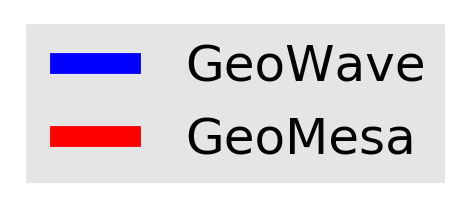
\includegraphics[width=0.20\textwidth]{../docs/img/legend.png}
%%   \caption{Legend.}
%%   \label{legend}
%% \end{wrapfigure}

\begin{figure}[h!tb]
  \centering
  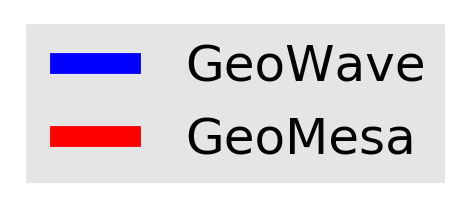
\includegraphics[width=0.20\textwidth]{../docs/img/legend.png}
  \caption{Legend.}
  \label{legend}
\end{figure}

\subsection{ GeoLife}

Test for GeoLife were performed on EMR 5.0.0 clusters of one m3.2xlarge master and three m3.2xlarge workers.
The GeoLife dataset was ingested with default 2D and 3D indexes for both systems.
See the appendix for details about machine specs and ingest results.

\subsubsection{Spatial queries of Beijing}

We used the Beijing geojson from Mapzen's borders dataset, which can be found in the resources of the \texttt{core} subproject.
This represents the multipolygon seen in Figure \ref{beijingpolygon}.

\begin{figure}[h!tb]
  \centering
  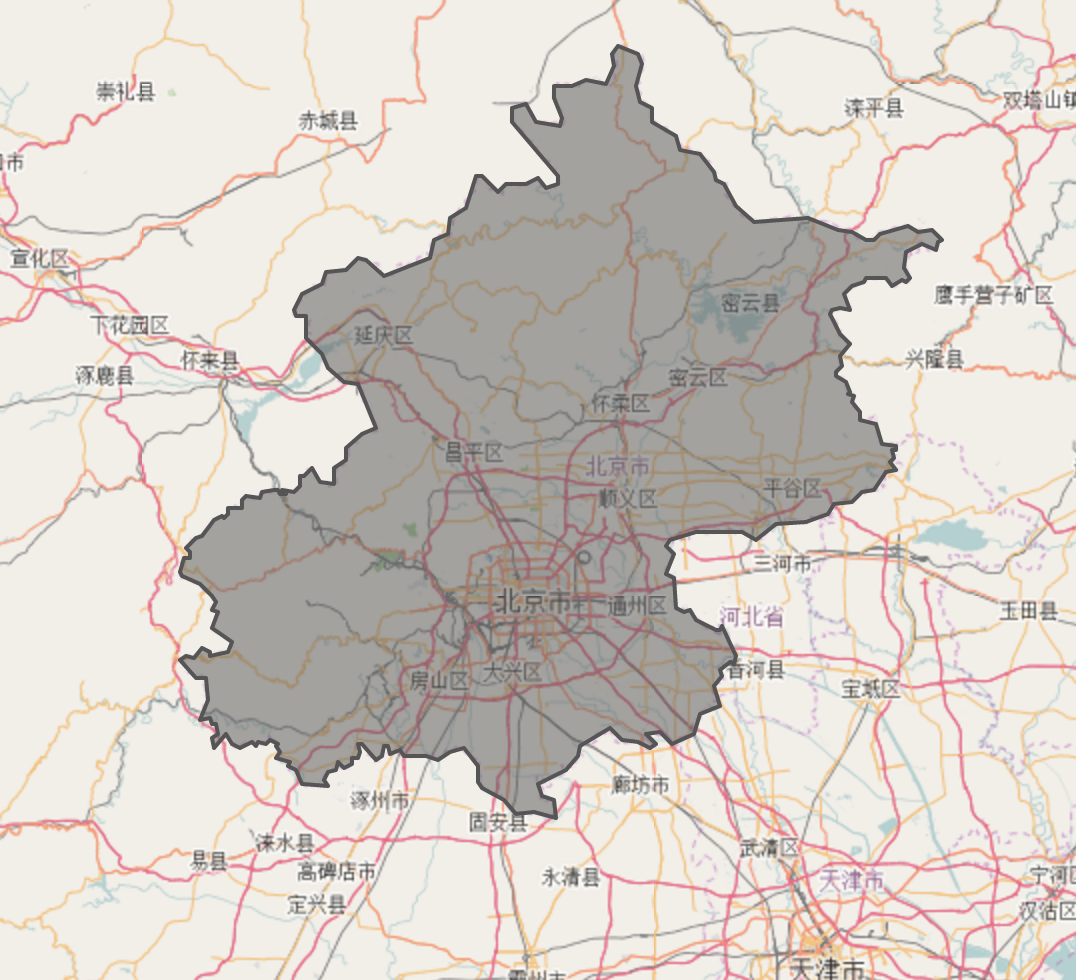
\includegraphics[width=0.60\textwidth]{../docs/img/beijing-poly.png}
  \caption{Beijing polygon.}
  \label{beijingpolygon}
\end{figure}

We then queried the city of Beijing over the whole time of the dataset.
We tracked results for both iterating over the resulting \texttt{SimpleFeature}s.
The timing results for that test, with outliers removed are shown in Figure \ref{beijingiterate}.

\begin{figure}[h!tb]
  \centering
  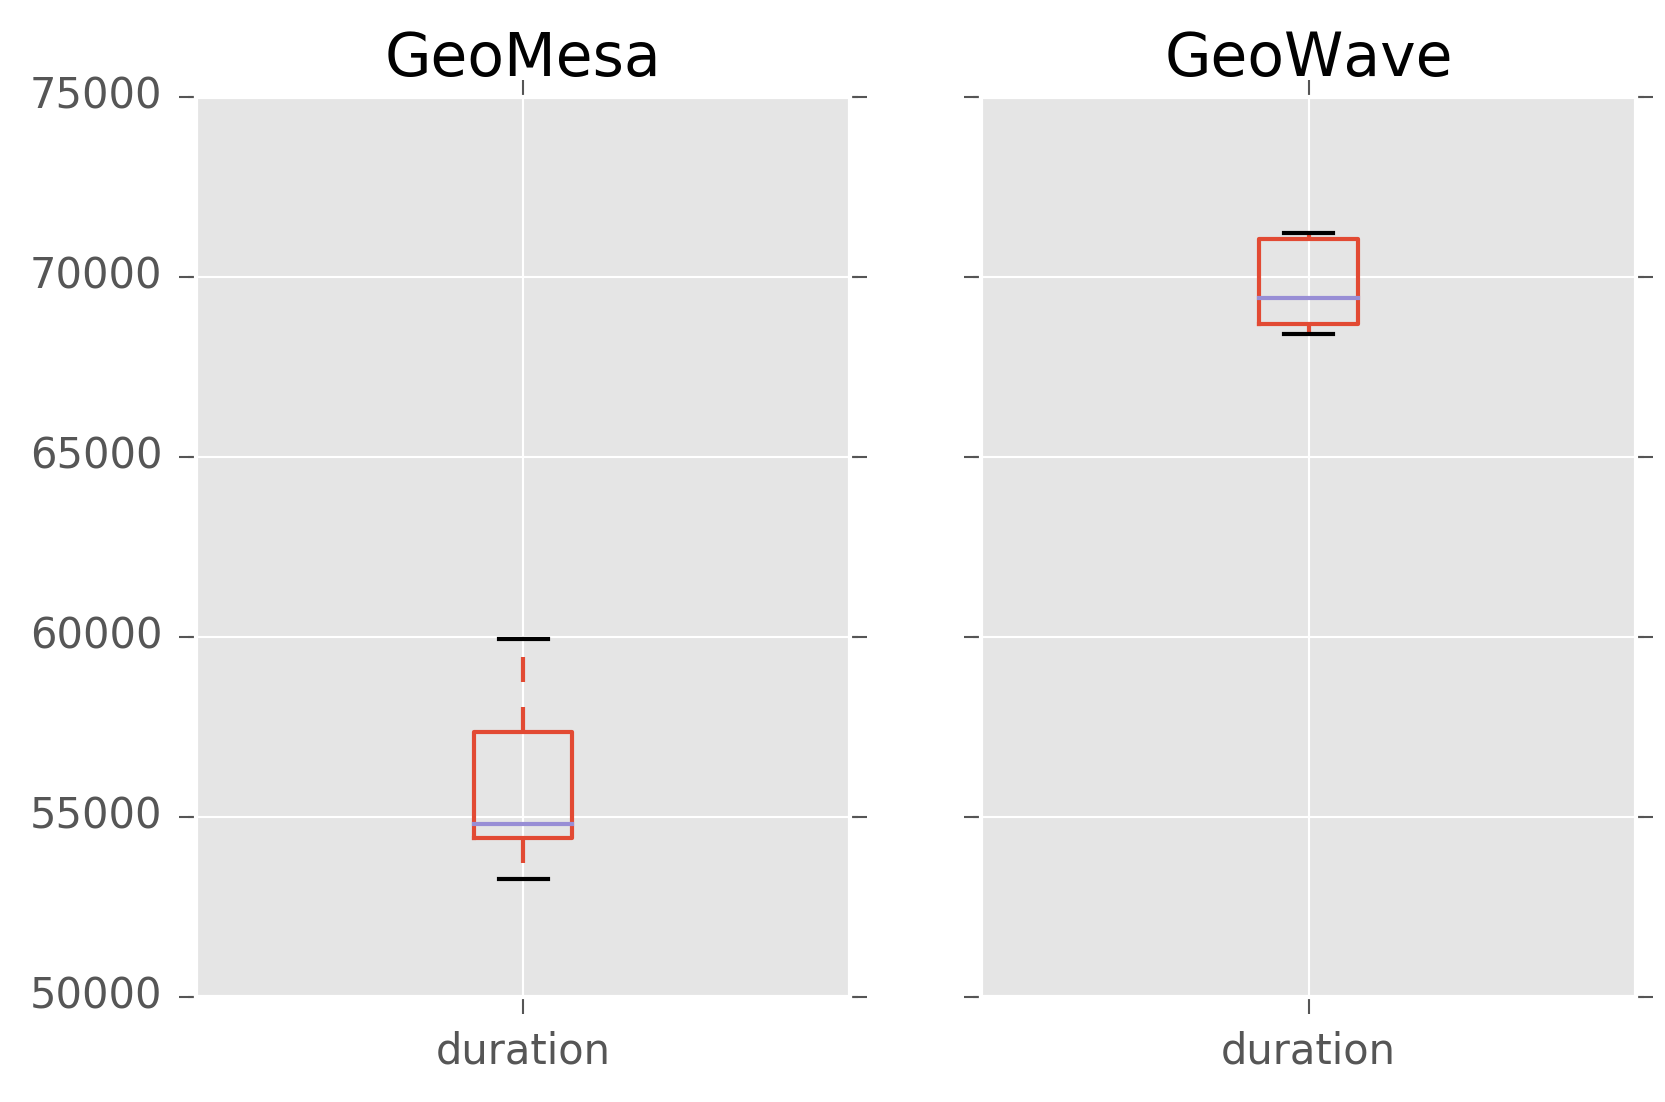
\includegraphics[width=0.60\textwidth]{../docs/img/geolife-beijing-iterate.png}
  \caption{Beijing iterations.}
  \label{beijingiterate}
\end{figure}

These queries take a long time; this makes sense, as they are iterating over $19,902,865$ results.

\subsubsection{Spatial queries of central Beijing}

To test on queries with smaller result set, we using \texttt{geojson.io} to draw a rough polygon around the center of Beijing.
We then performed spatial-only queries using the polygon shown in Figure \ref{beijingcenter}.

\begin{figure}[h!tb]
  \centering
  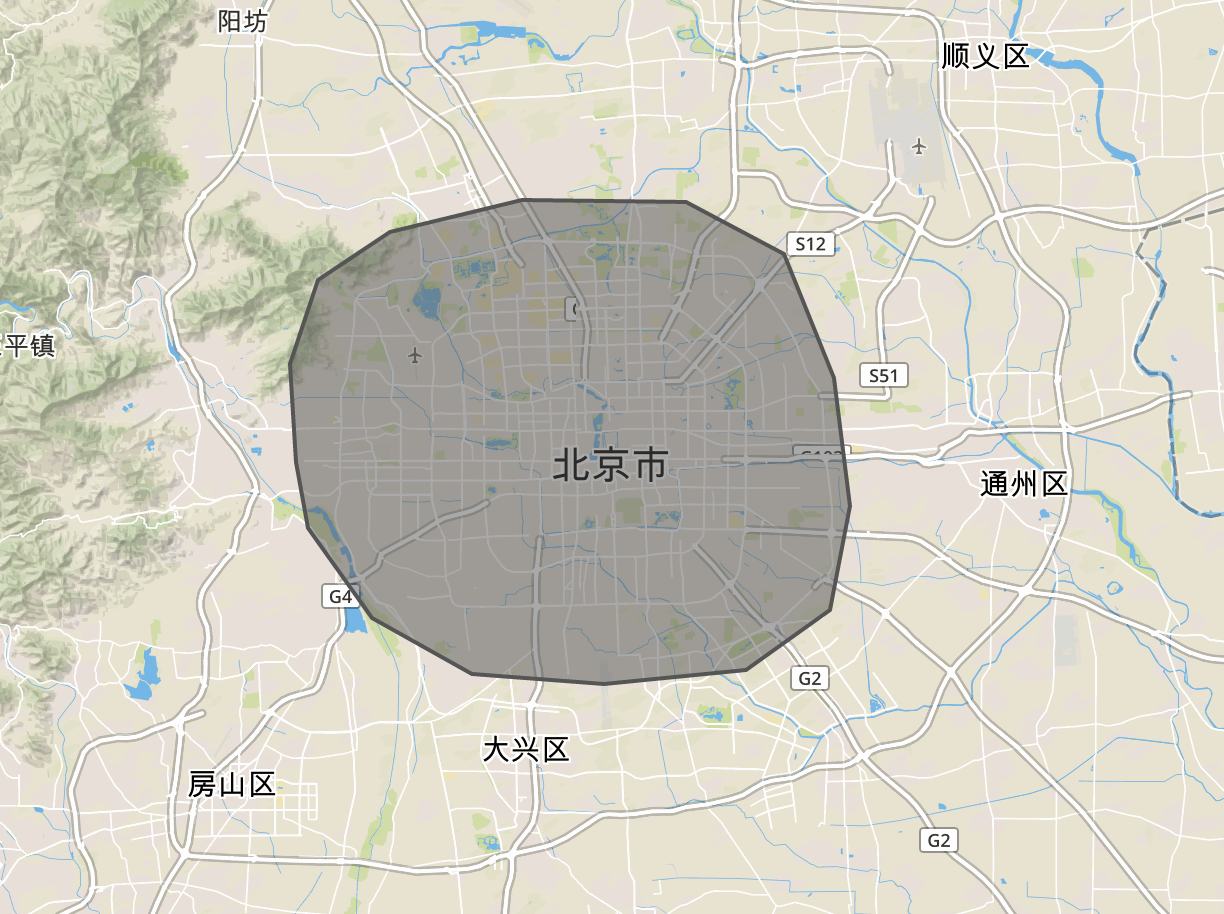
\includegraphics[width=0.60\textwidth]{../docs/img/beijing-center.png}
  \caption{Beijing center.}
  \label{beijingcenter}
\end{figure}

This allowed us to track the iteration and count queries against a smaller spatial extent.
However, this query did not actually cut out too many results; the result set for this query included $16,624,351$ results.
In Figure \ref{beijingcenteriterate}, outliers have been removed.

\begin{figure}[h!tb]
  \centering
  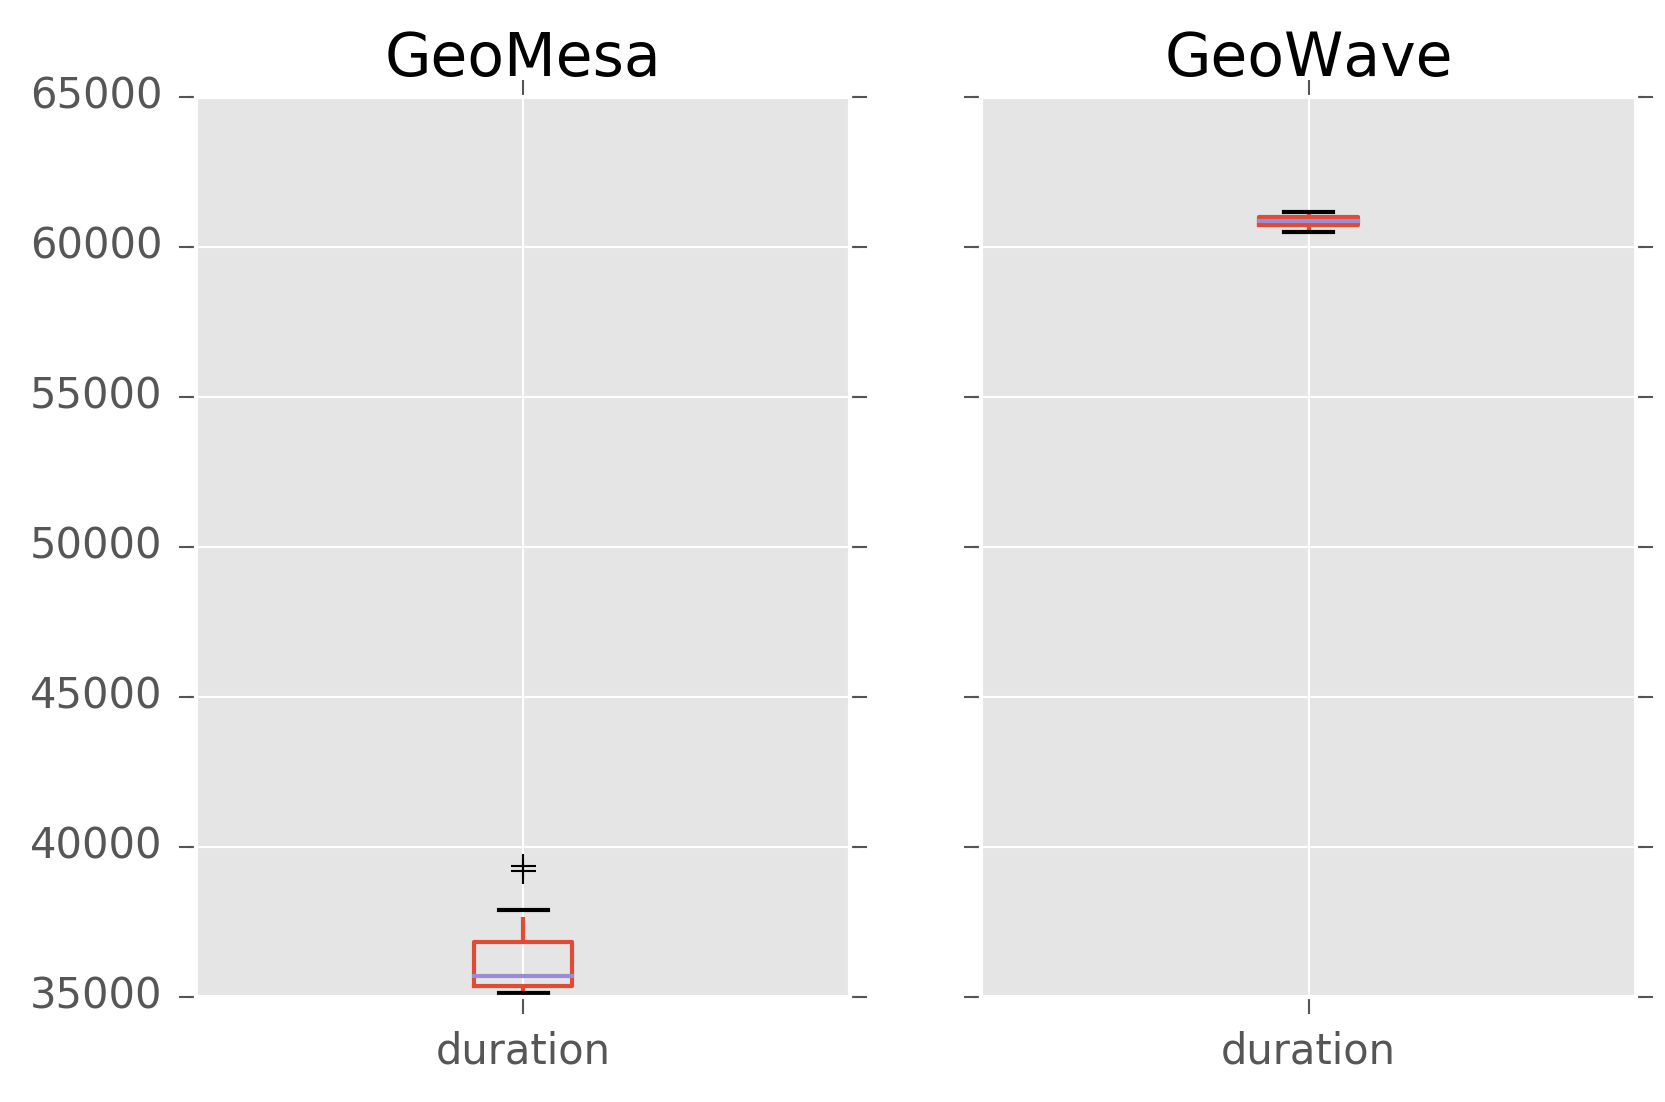
\includegraphics[width=0.60\textwidth]{../docs/img/geolife-beijing-center-iterate.png}
  \caption{Beijing center iterations.}
  \label{beijingcenteriterate}
\end{figure}

These two results show GeoMesa handling queries with large results faster than GeoWave, which is a result we've seen fairly consistently in our tests.

\subsubsection{Spatial queries of bounding boxes across Beijing}

This query cuts the bounding box of Beijing into \texttt{N} equal sized bounding boxes,
represented by the tile coordinate \texttt{COL} and \texttt{ROW}.

For instance, running \texttt{N=32} would create bounding boxes that look like those shown in Figure \ref{beijingbbox32}.

\begin{figure}[h!tb]
  \centering
  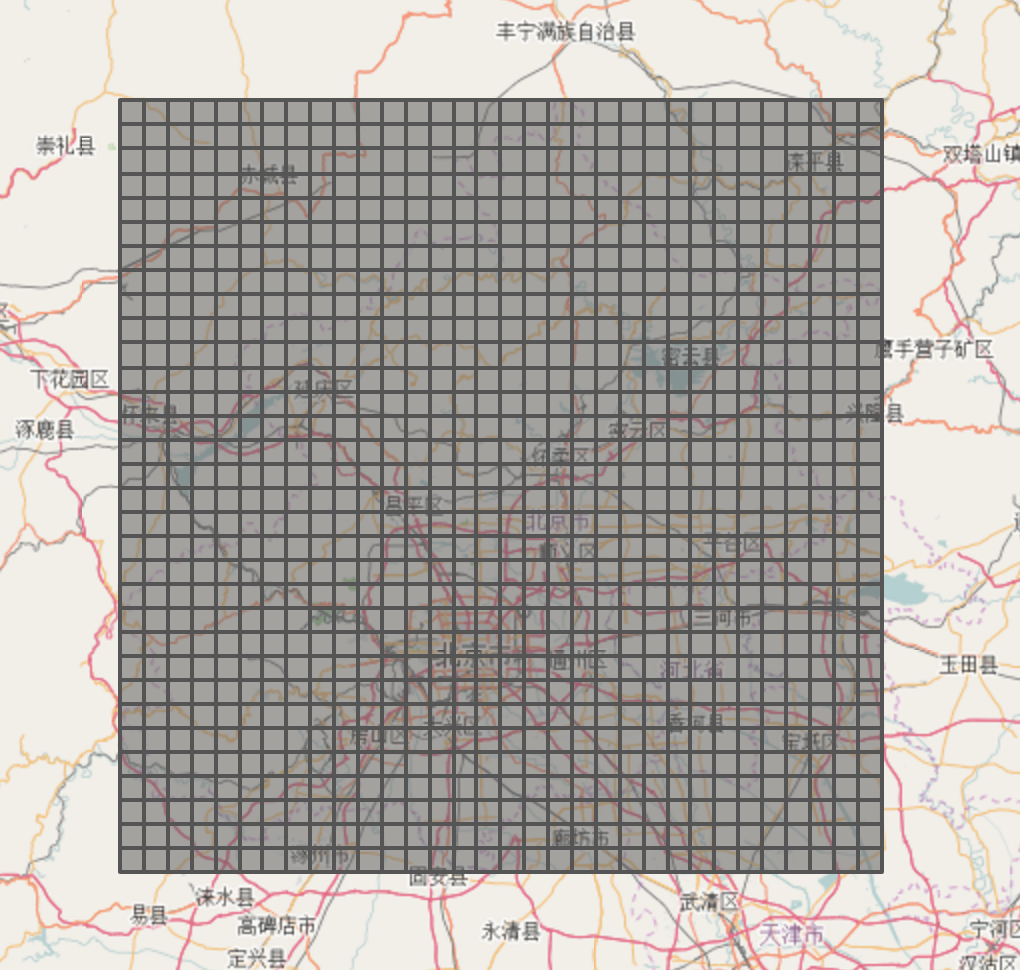
\includegraphics[width=0.60\textwidth]{../docs/img/beijing-bbox-32.png}
  \caption{Beijing bounding box for \texttt{N=32}.}
  \label{beijingbbox32}
\end{figure}

We tested with \texttt{N=32} \texttt{\{ 2, 4, 8, 16, 32\}}. This produced $1,024$ unique queries.
$417$ were queries with $0$ results, and were not considered.
$103$ of these queries did not produce the same result between GeoMesa and GeoWave;
a query for the entire bounding box of Beijing produces the same results,
so it is unclear why this mismatch occurs, and which system is incorrect.
Because these tests are focused on performance and not accuracy, these mismatched results are included in the graphs below.

The graph in Figure \ref{beijingscatter} plots the result count of each query against the duration of that query per system:

\begin{figure}[h!tb]
  \centering
  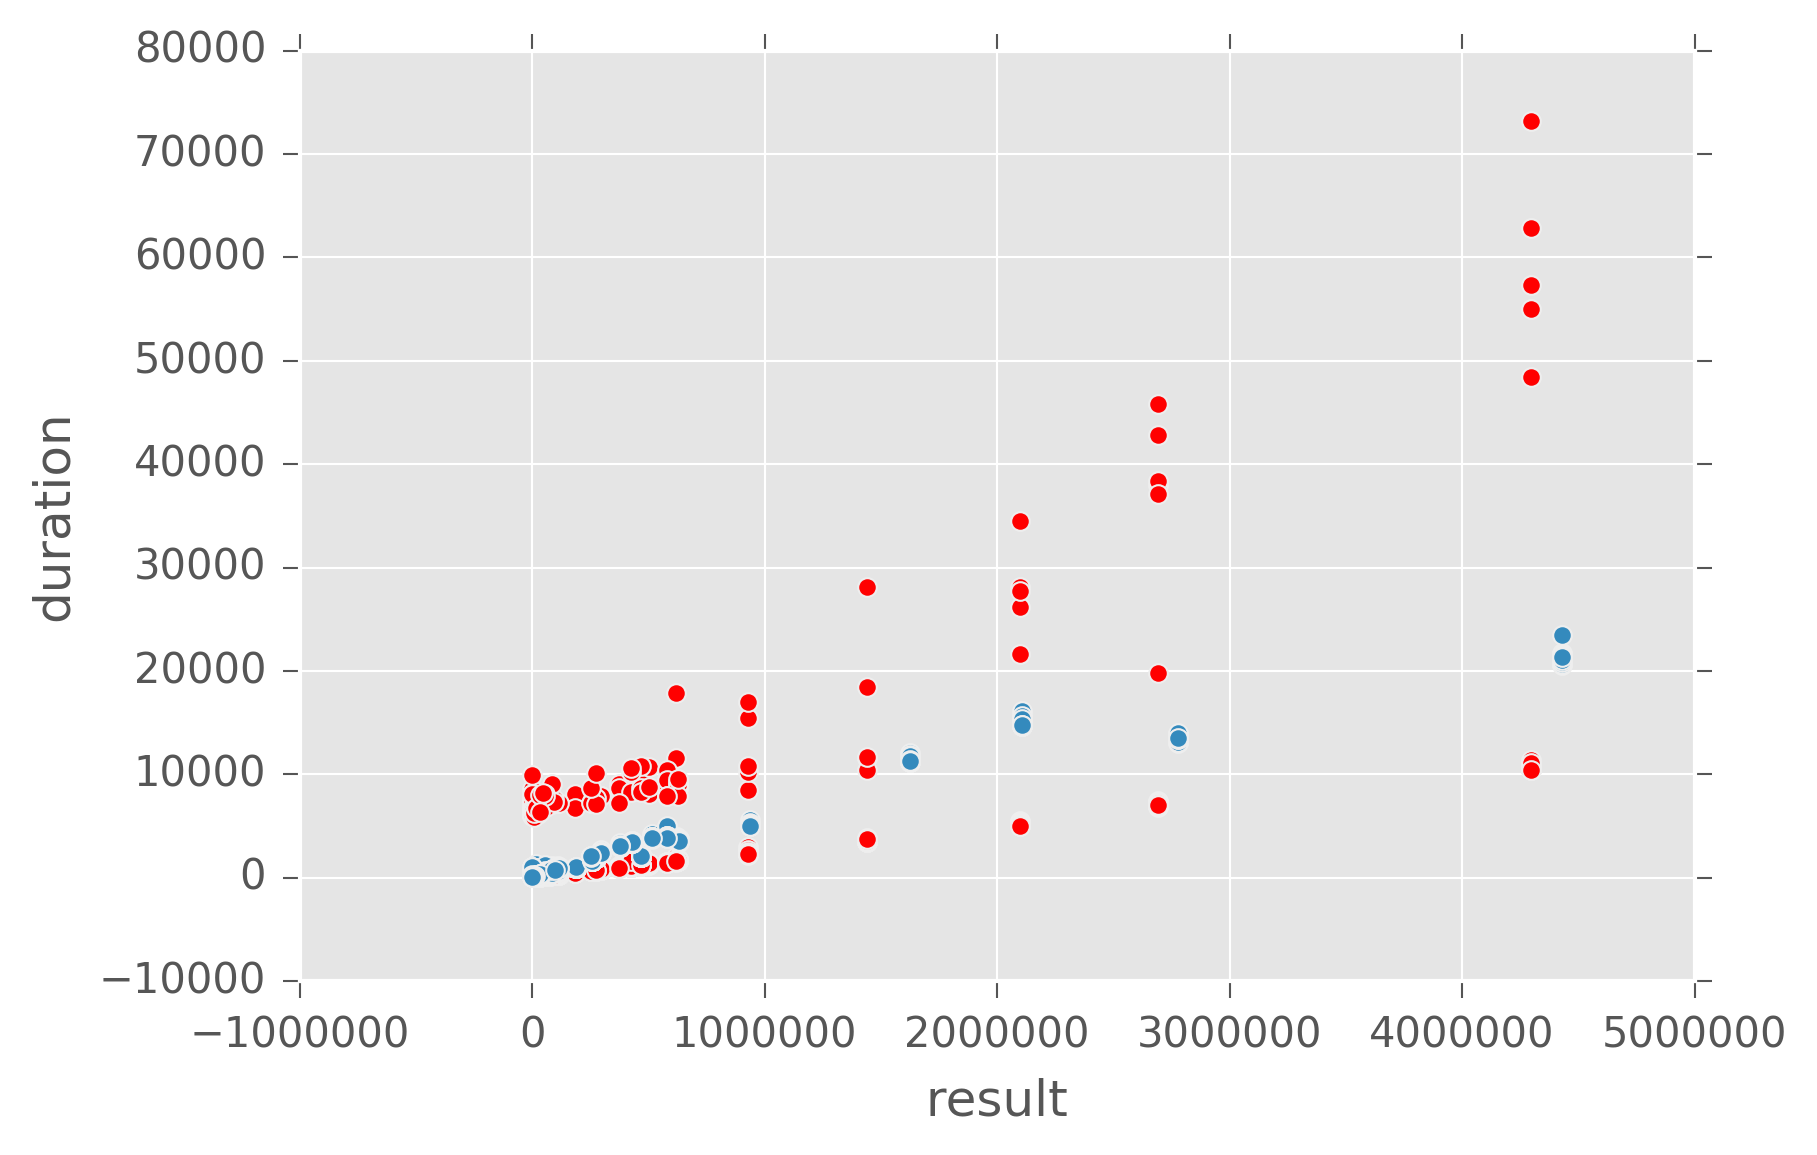
\includegraphics[width=0.60\textwidth]{../docs/img/geolife-bbox-scatter.png}
  \caption{Beijing iteration scatter plot.}
  \label{beijingscatter}
\end{figure}

This shows GeoMesa having more variance over duration; however it does not give a good indication of trends.
If we plot a linear regression on the two set of points, we can see that although GeoMesa appears to have
more variance in query duration, the queries typically return faster from GeoMesa than from GeoWave, and this
trend becomes more pronounced as the number of results increases (please see Figure \ref{beijingscatterreg}).

\begin{figure}[h!tb]
  \centering
  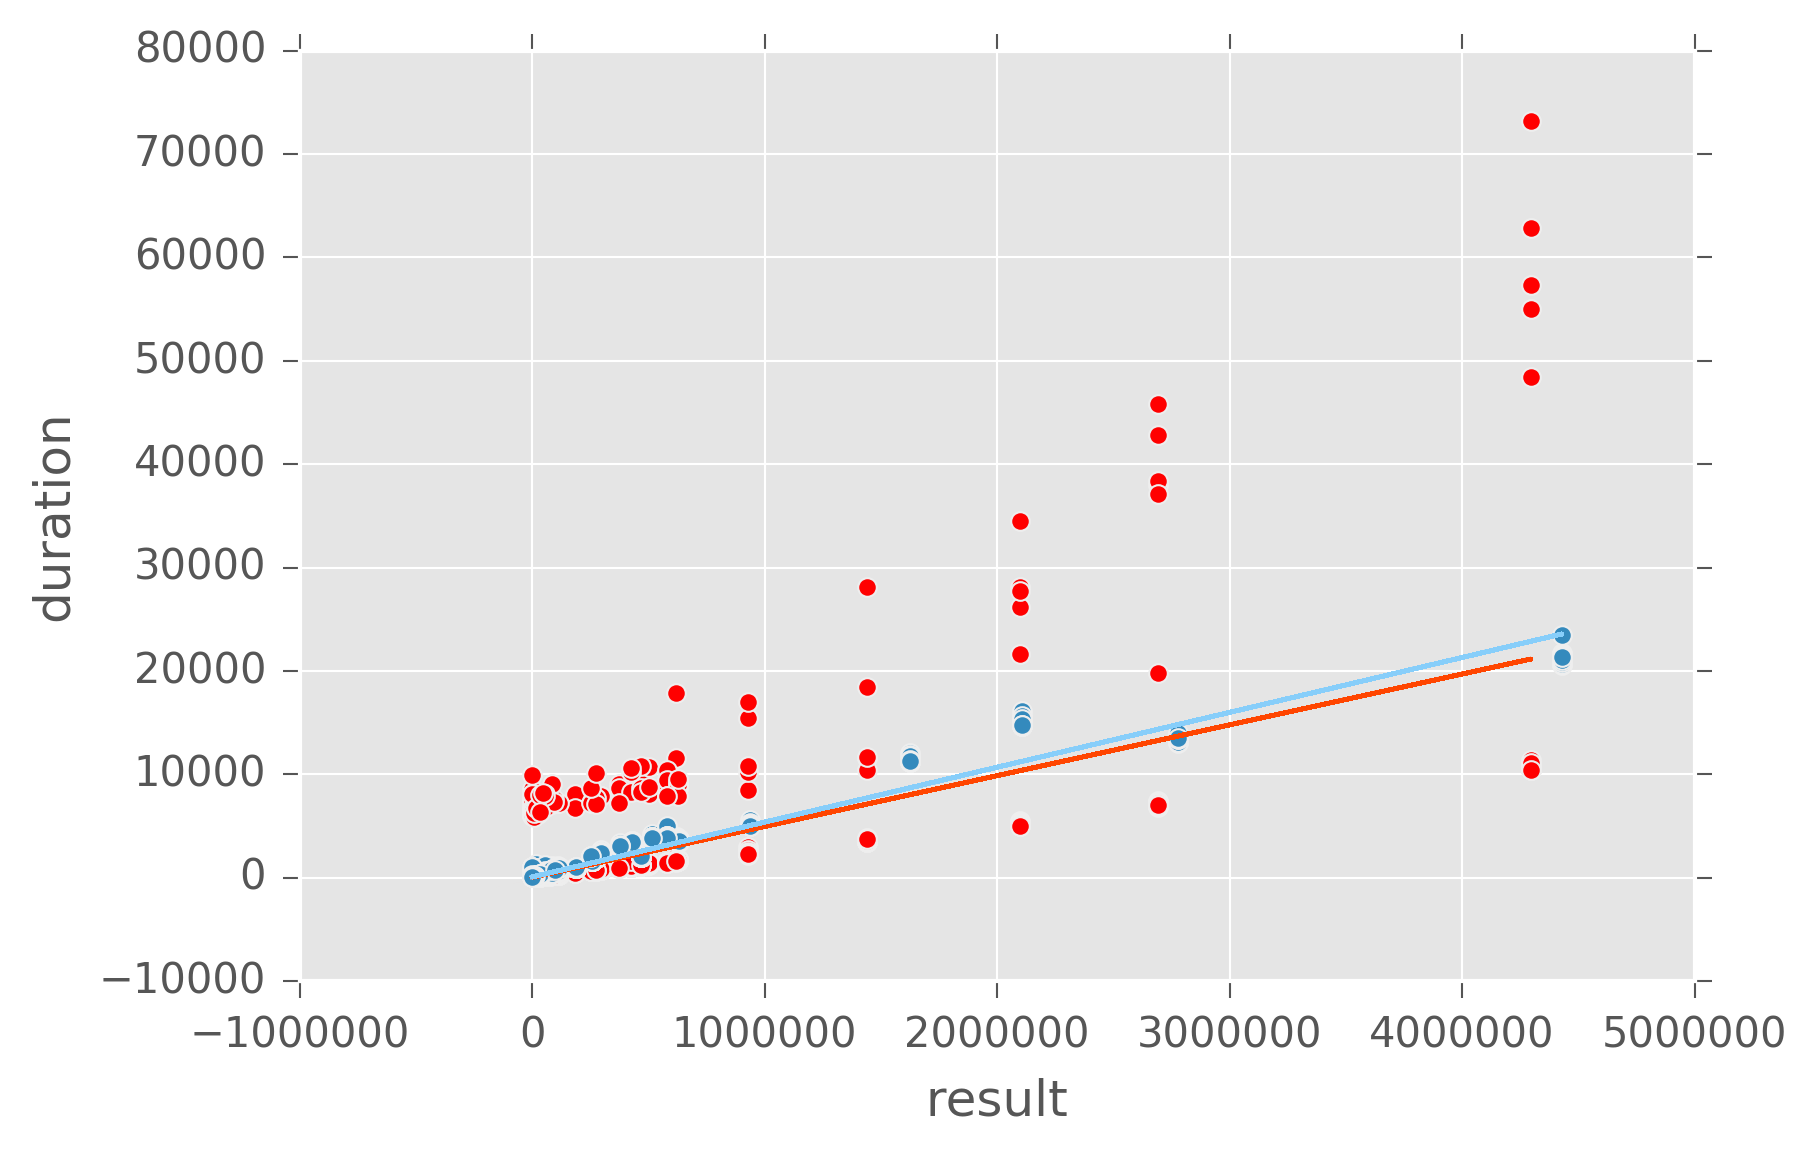
\includegraphics[width=0.60\textwidth]{../docs/img/geolife-bbox-scatter-with-regression.png}
  \caption{Beijing iteration scatter plot with regression.}
  \label{beijingscatterreg}
\end{figure}

GeoMesa has a feature called ``loose bbox'' that allows you to trade performance for result accuracy;
it only uses the space filling curve to filter data and does no secondary filtering, so false positives
could be returned. The graph below includes a scatterplot and regression for the loose bounding box queries in yellow
(please see Figure \ref{beijingloosescatterreg}).

\begin{figure}[h!tb]
  \centering
  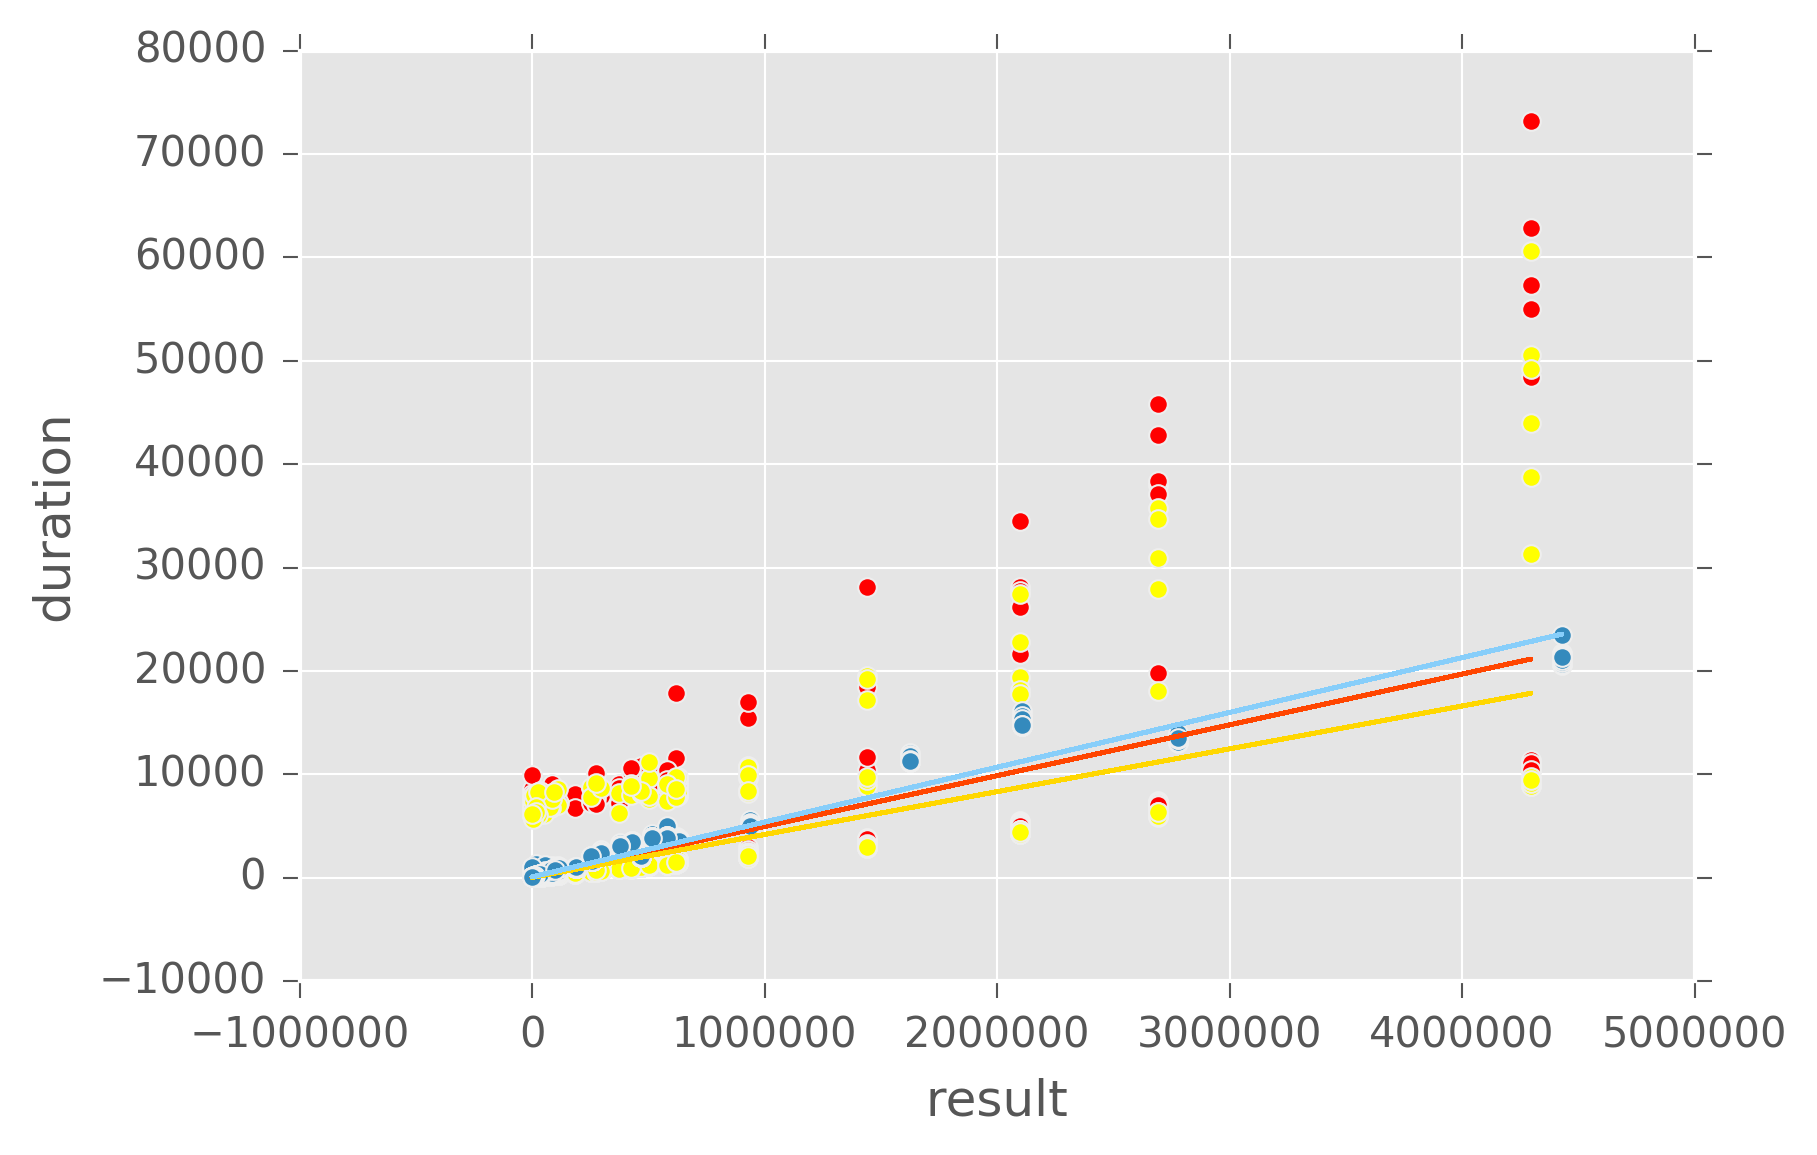
\includegraphics[width=0.60\textwidth]{../docs/img/geolife-bbox-regression-with-loose.png}
  \caption{Beijing ``loose bbox'' scatter plot with regression.}
  \label{beijingloosescatterreg}
\end{figure}

The graph in Figure \ref{beijingloosescatterreg2} shows the regressions against queries returning less than $10,000$ results.
It shows that even for queries with lower result counts, GeoMesa tends to slightly outperform GeoWave
for these spatial-only point data queries, for both loose and exact queries.

\begin{figure}[h!tb]
  \centering
  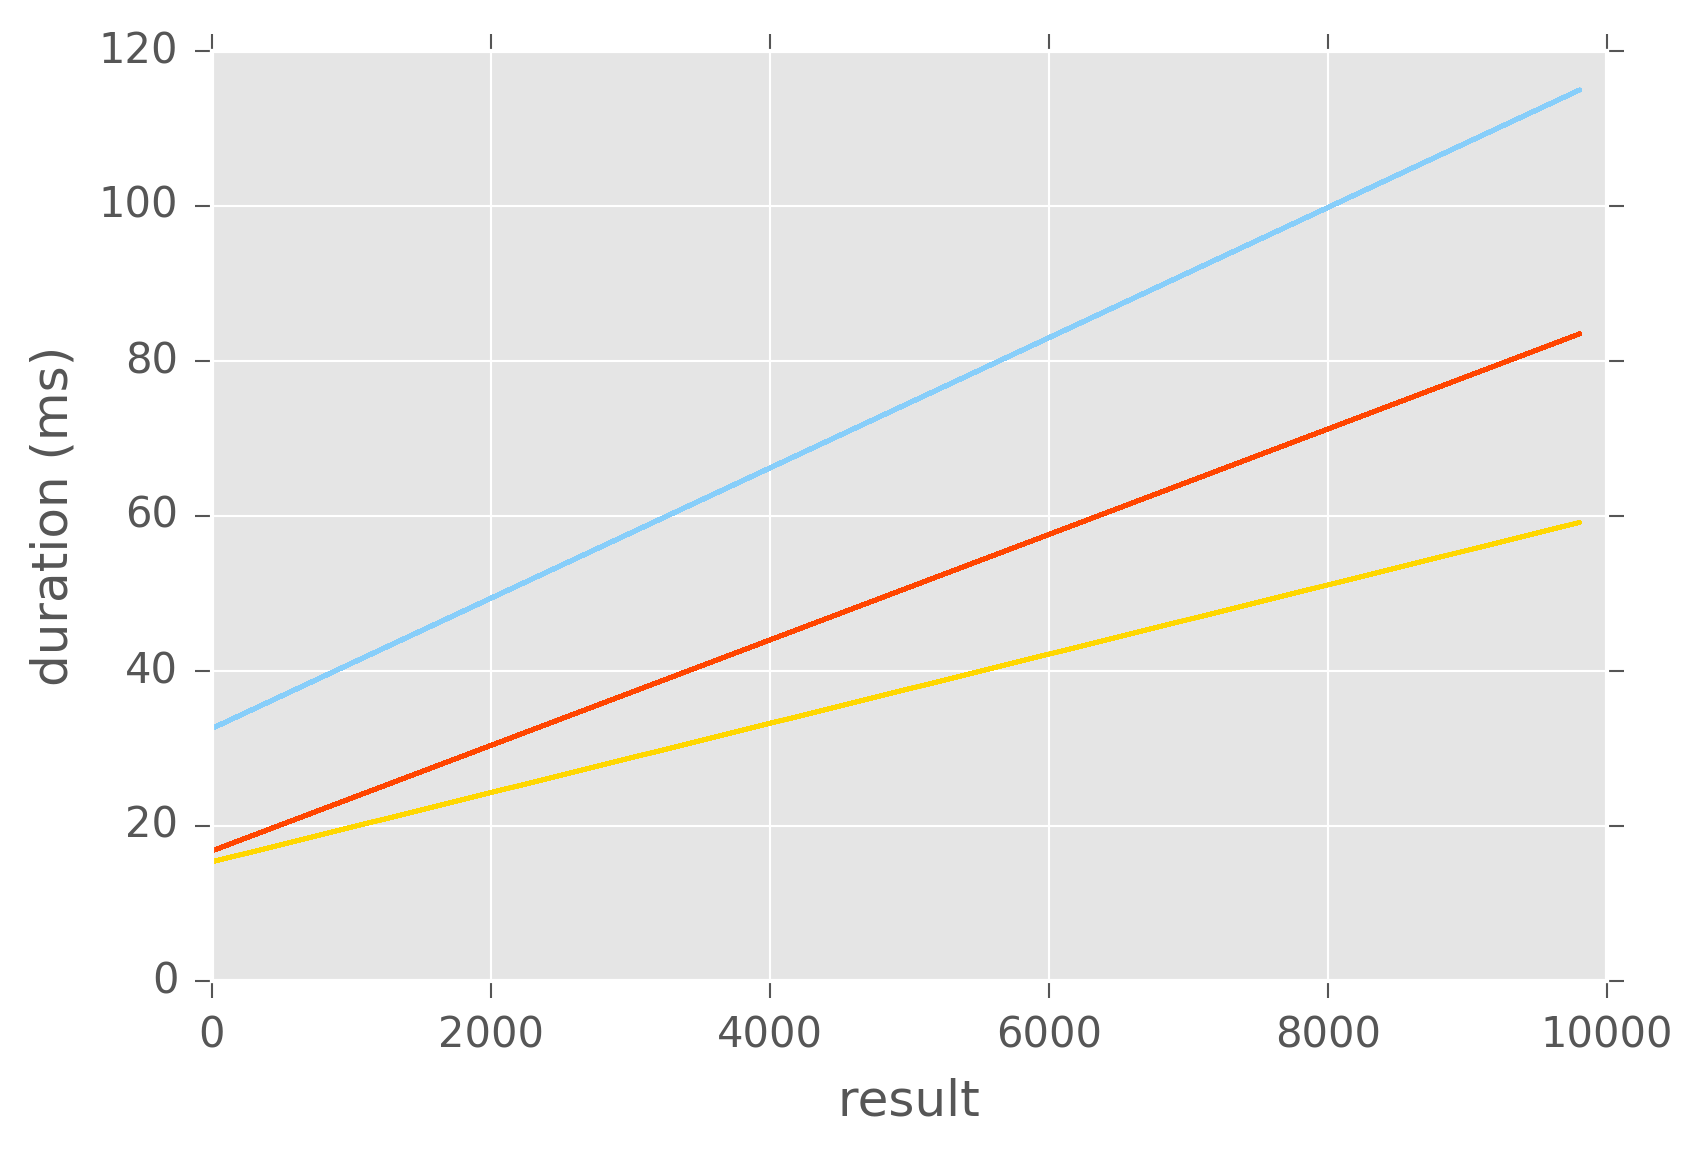
\includegraphics[width=0.60\textwidth]{../docs/img/geolife-bbox-regression-with-loose-less-than-10000.png}
  \caption{Beijing ``loose bbox'' scatter plot with regression, fewer than $10,000$ results.}
  \label{beijingloosescatterreg2}
\end{figure}

\subsubsection{Spatiotemporal query results}

In both systems, spatiotemporal queries (those with bounds in both space and time) hit a different table and indexing mechanism than the spatial-only queries described above.
To include a temporal aspect to our queries, we ran a query over the center of Beijing for the month of August in 2011.
This returned $84,496$ results.
In Figure \ref{beijingjan2011}, outliers have been removed.

\begin{figure}[h!tb]
  \centering
  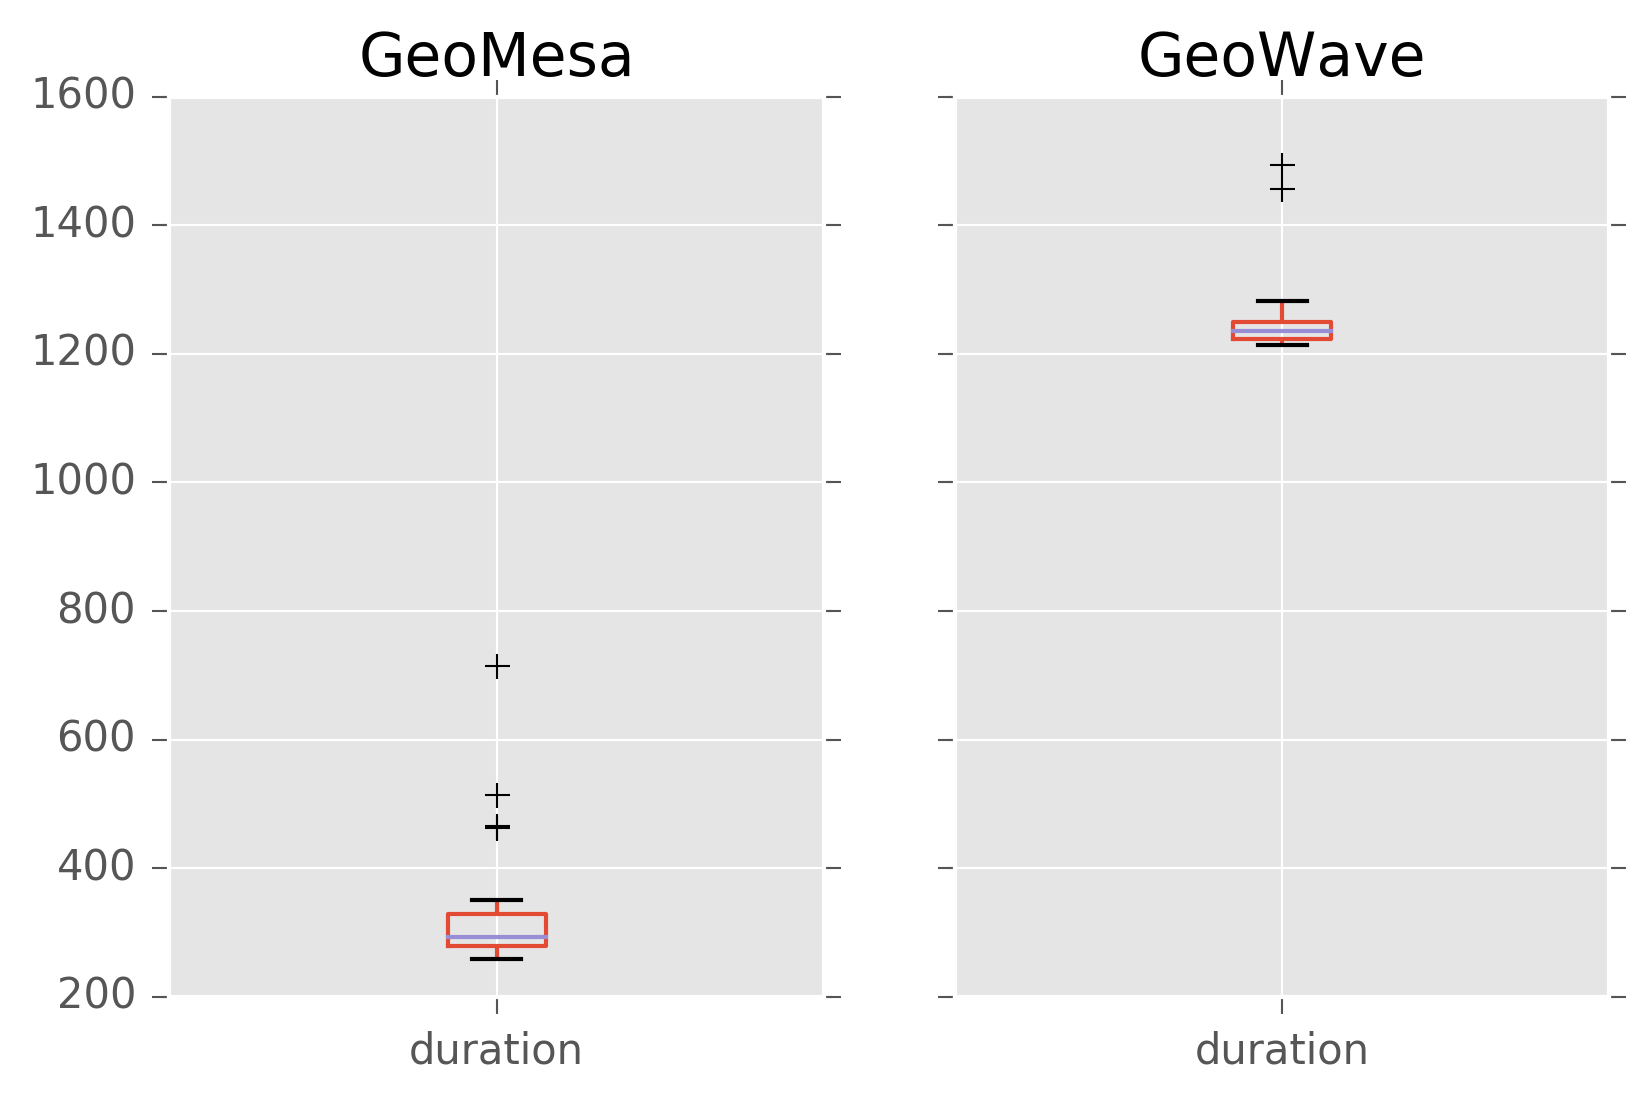
\includegraphics[width=0.60\textwidth]{../docs/img/geolife-beijing-center-aug-2011.png}
  \caption{Beijing January 2011 iterations.}
  \label{beijingjan2011}
\end{figure}

We see that GeoMesa performs better in this query.
If we plot the histogram of GeoMesa durations with outliers removed,
for both exact and loose (red and yellow, respectively), and compare it to the histogram of durations for GeoWave queries with outliers removed,
we see that there is a wider spread of timing results coming from GeoWave for this query.

\begin{figure}[h!tb]
  \centering
  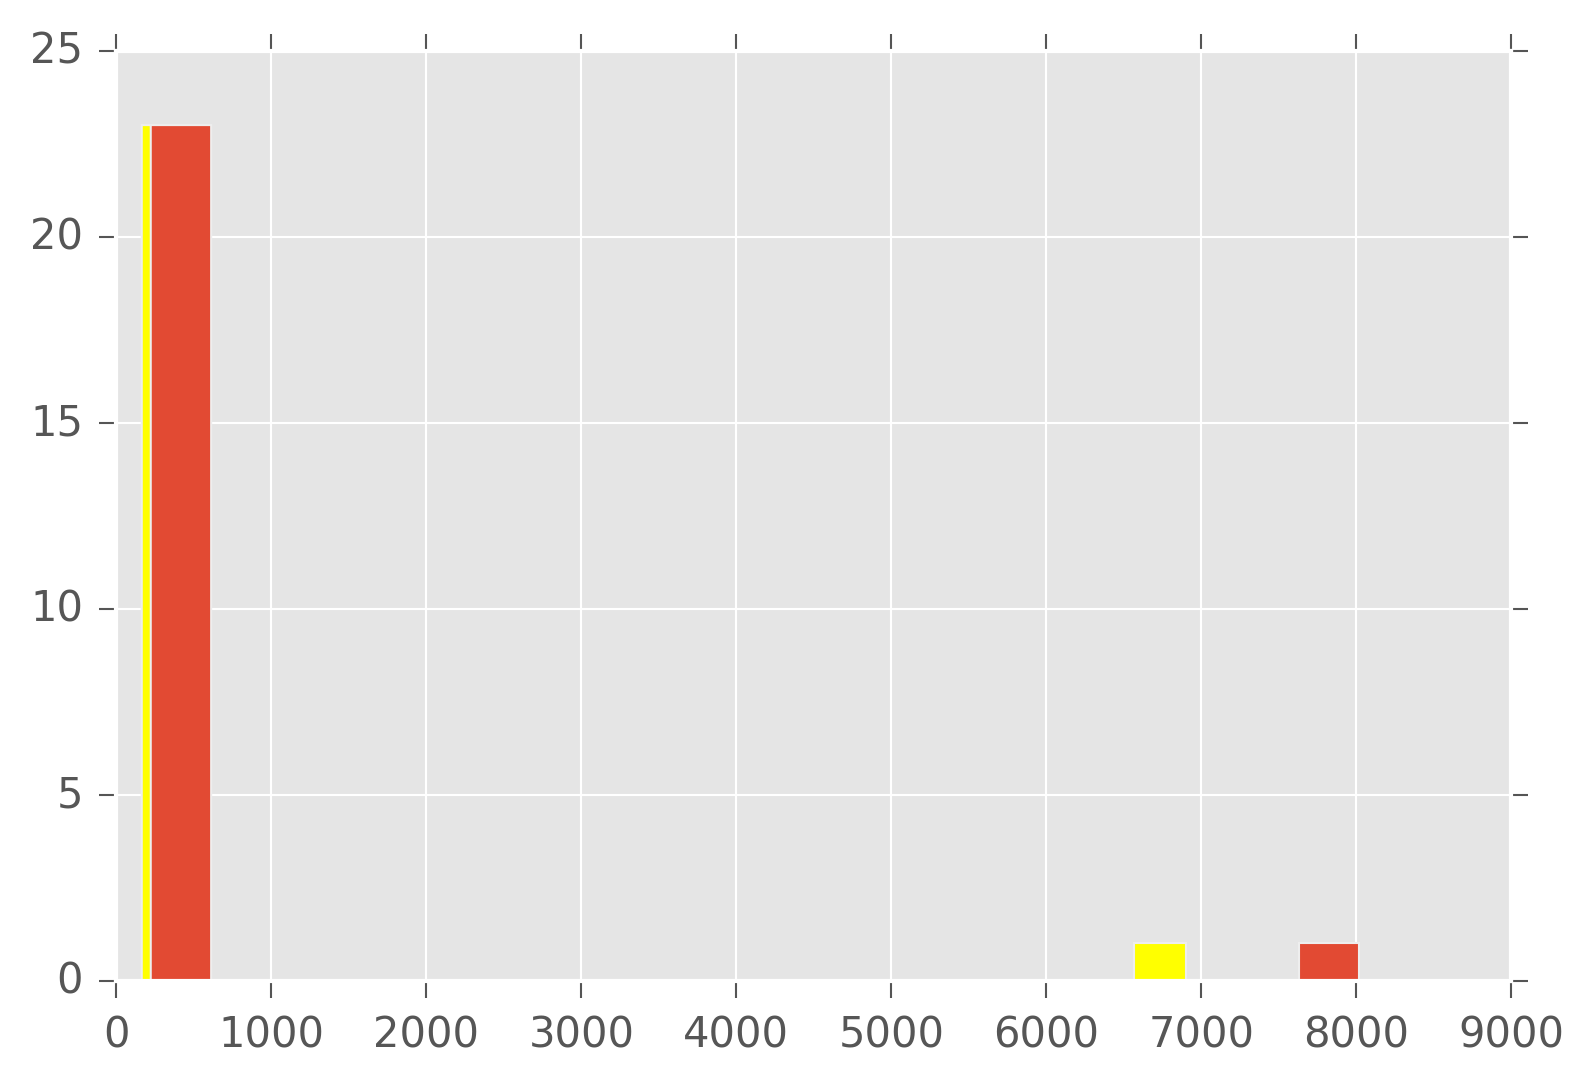
\includegraphics[width=0.45\textwidth]{../docs/img/geolife-beijing-center-feb-2011-bbox-gm.png}
  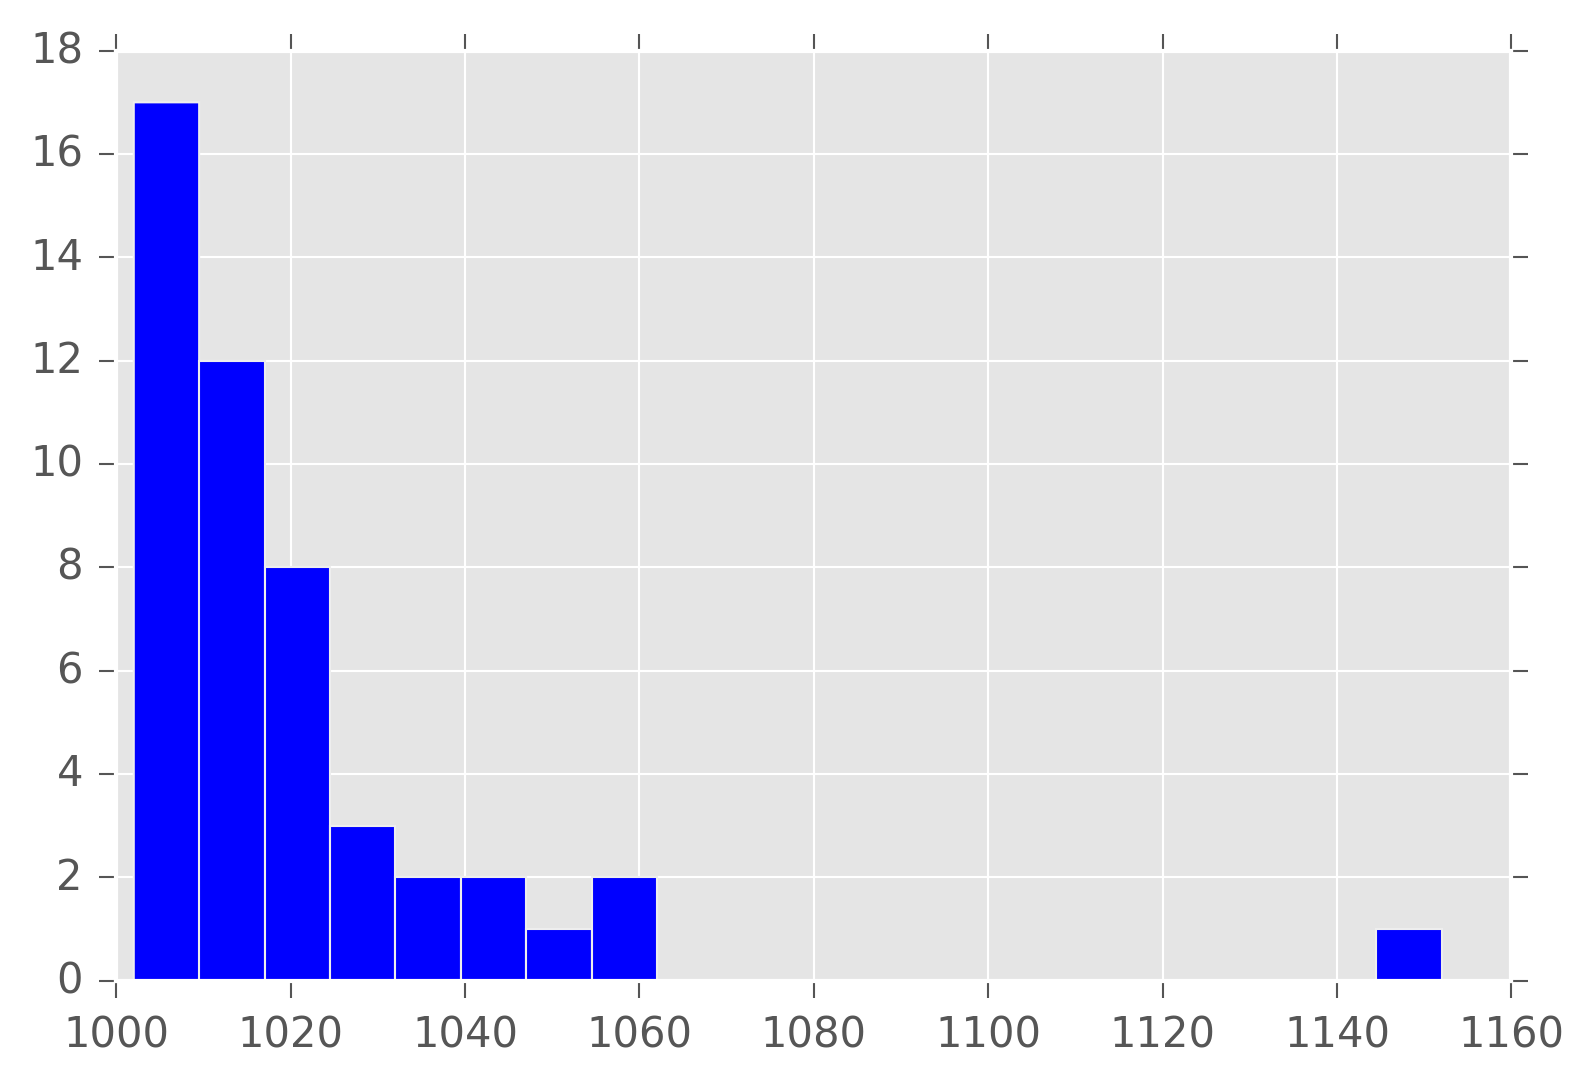
\includegraphics[width=0.45\textwidth]{../docs/img/geolife-beijing-center-feb-2011-bbox-gw.png}
  \caption{Beijing February 2011 iterations.}
  \label{beijingfebg2011}
\end{figure}


\subsection{GDELT}

Test for GDELT were performed on EMR 5.0.0 clusters of one \texttt{m3.2xlarge} master and five \texttt{m3.2xlarge} workers.

\subsubsection{Spatiotemporal queries of areas around cities: City Buffers}

For these queries, which we call the ``city buffer'' tests, queries are taken from center points corresponding to the following cities:
Paris, Philadelphia, Istanbul, Baghdad, Tehran, Beijing, Tokyo, Oslo, Khartoum, and Johannesburg.
For instance, the Paris city buffers can be seen in Figure \ref{paris}.

\begin{figure}[h!tb]
  \centering
  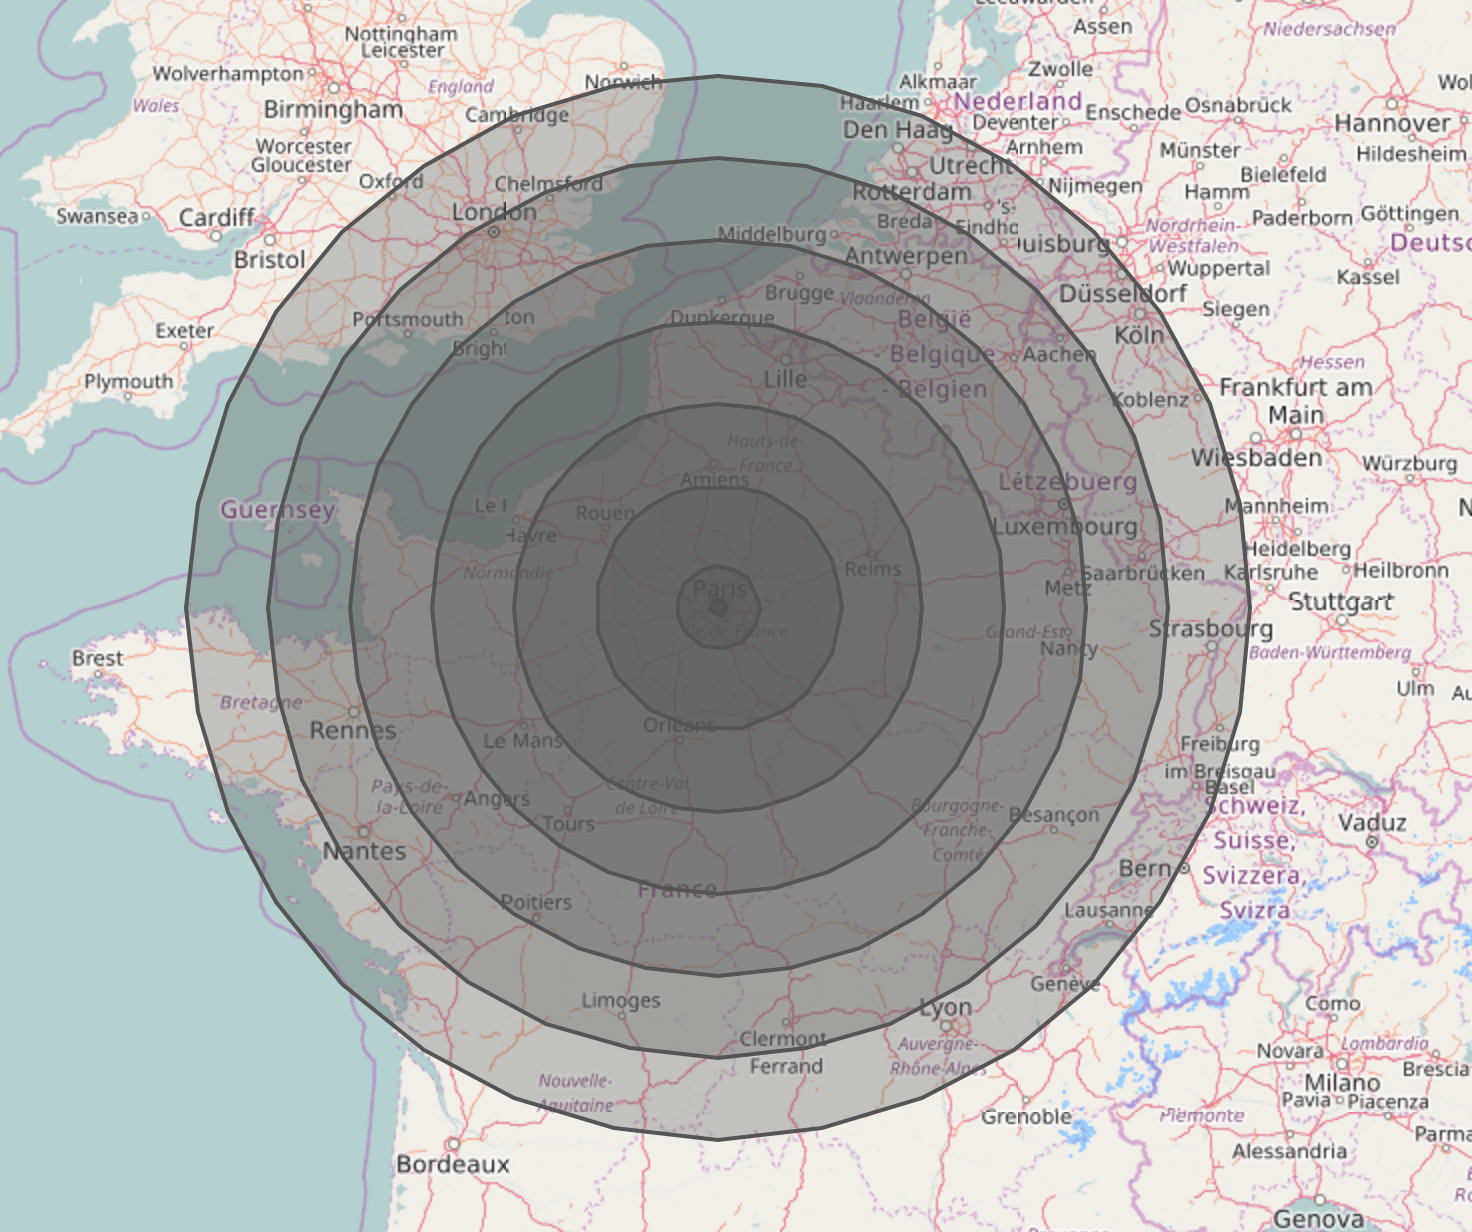
\includegraphics[width=0.60\textwidth]{../docs/img/gdelt/paris-city-buffers.png}
  \caption{Paris city buffers.}
  \label{paris}
\end{figure}

The queries were taken over a set of these durations: six months, two months, two weeks, and six days.

Figure \ref{durationbyresult} contains a scatter plot of duration by query result count.

\begin{figure}[h!tb]
  \centering
  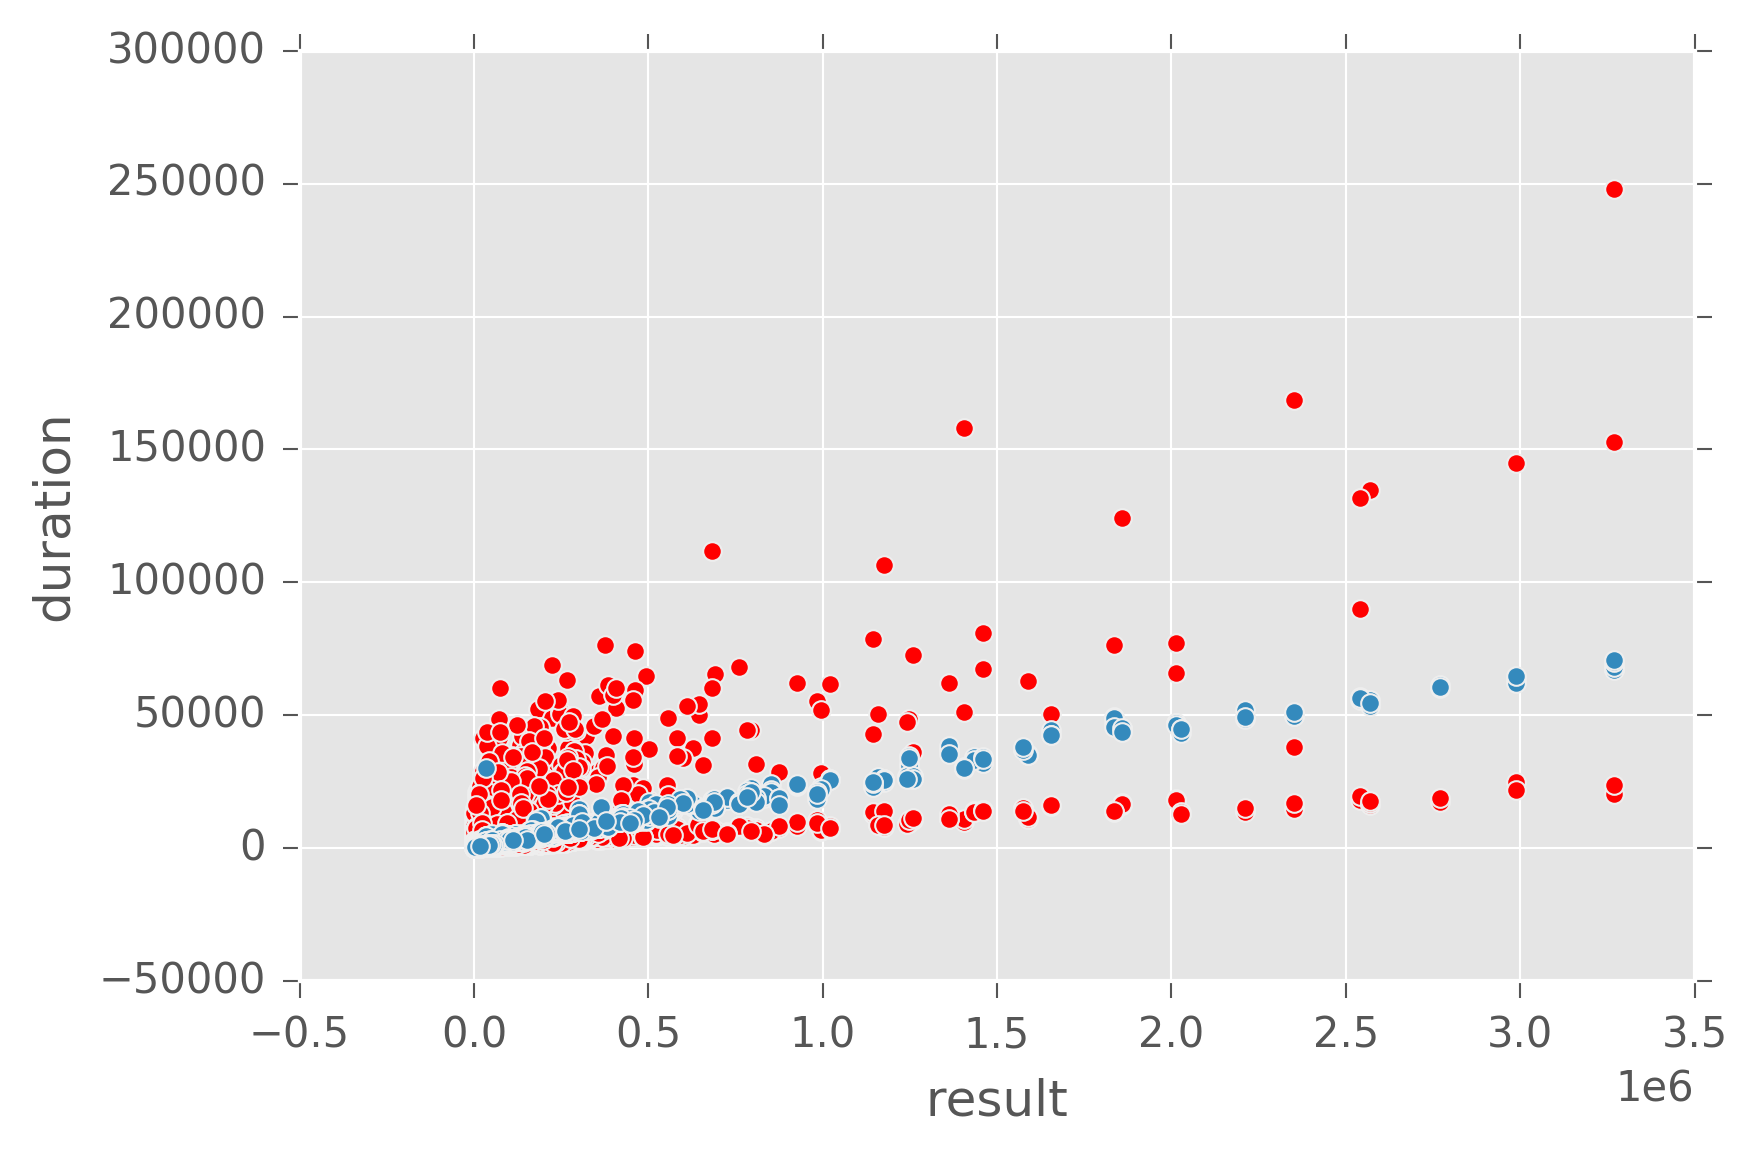
\includegraphics[width=0.60\textwidth]{../docs/img/gdelt/gdelt-result-over-duration.png}
  \caption{Duration by result count.}
  \label{durationbyresult}
\end{figure}

We can see that GeoMesa has much less consistent results than GeoWave.
If we plot a linear regression on this point sets, we'll get what is shown in Figure \ref{durationbyresultreg}.

\begin{figure}[h!tb]
  \centering
  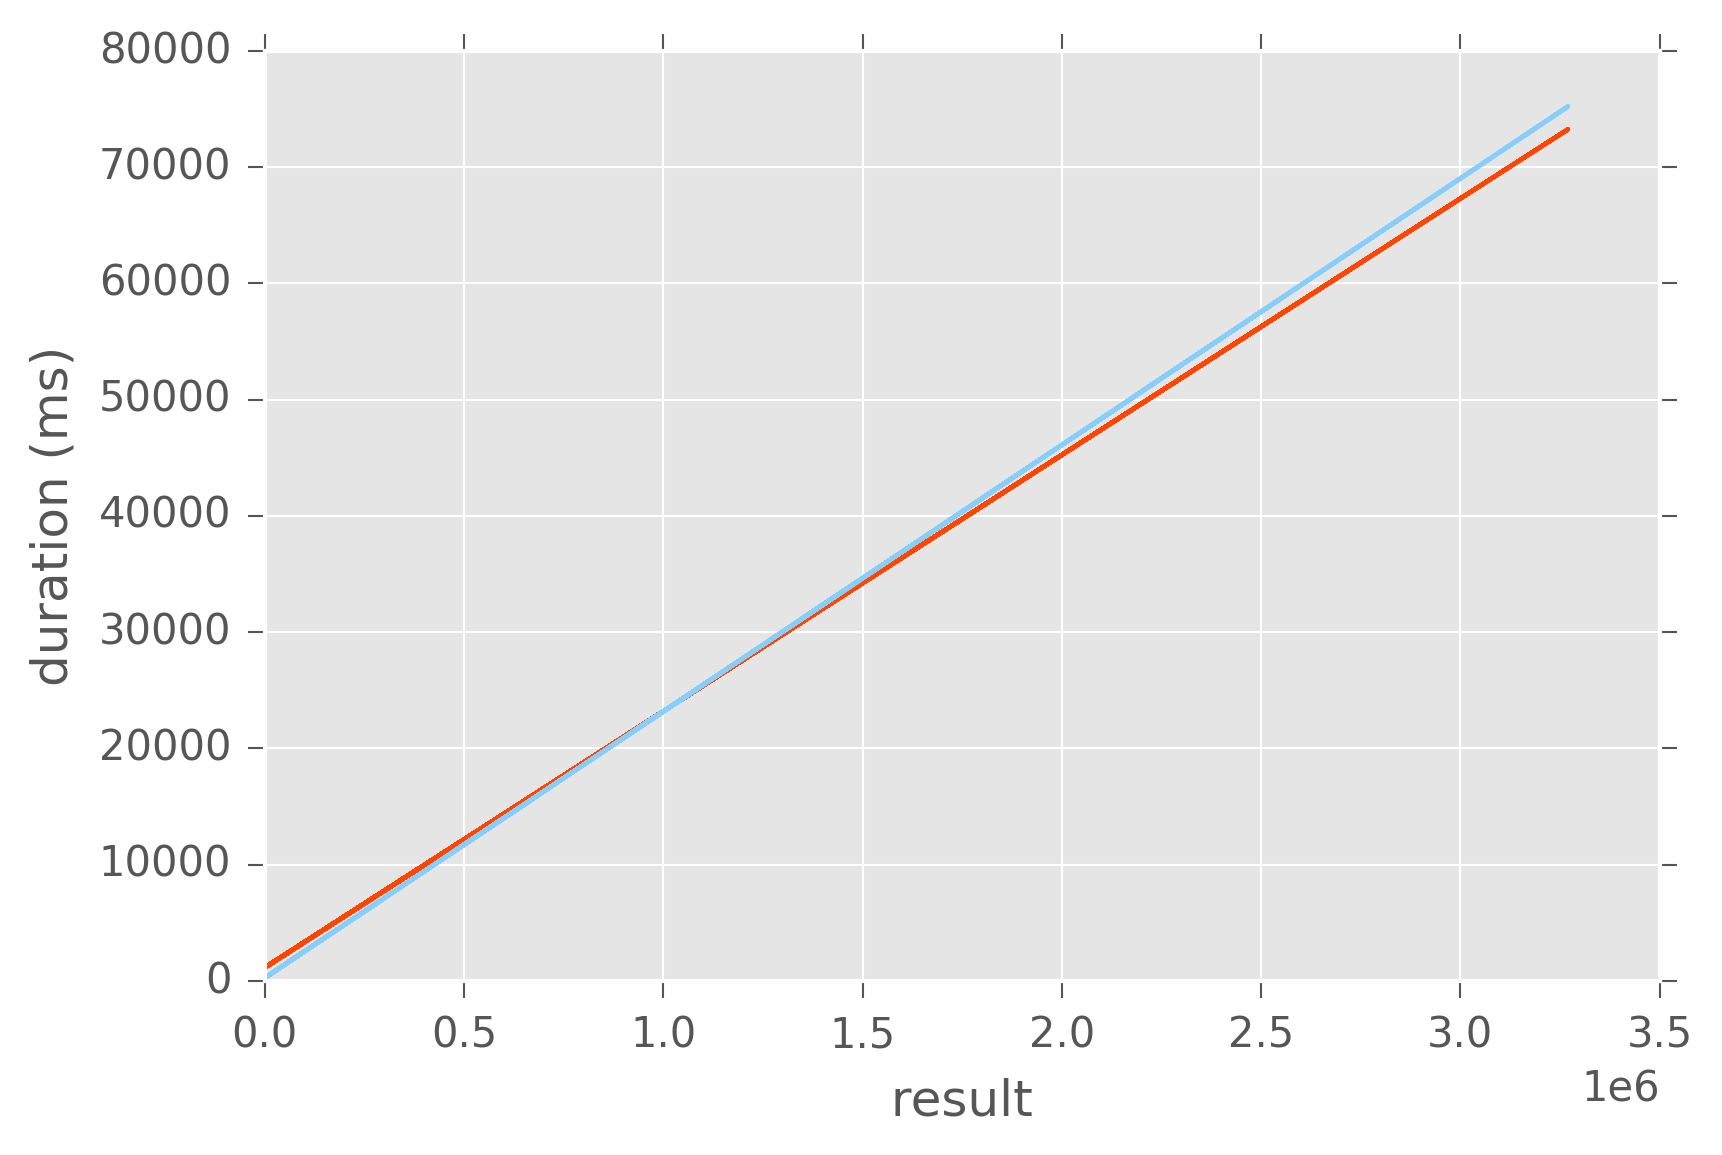
\includegraphics[width=0.60\textwidth]{../docs/img/gdelt/gdelt-result-over-duration-regression.png}
  \caption{Duration by result regression.}
  \label{durationbyresultreg}
\end{figure}

GeoMesa tends to be slower at returning these queries than GeoWave, until the queries return a large number of results.
According to the regression, after around 1 million results returned, GeoMesa becomes faster than GeoWave.
This is an imprecise result, but one that we have found consistent over point datasets: GeoMesa generally does better with queries that produce large result sets.

Figure \ref{durationresultall14} shows the mean duration of queries over all cities and all buffer sizes, for 14 day queries, based on the result count of the queries.
The $x$-axis in this case represents a bin of result counts;
points were averaged according to a quantile-based discretization function of result count,
which is represented here on the $x$-axis as the lowest result count of that grouping.

\begin{figure}[h!tb]
  \centering
  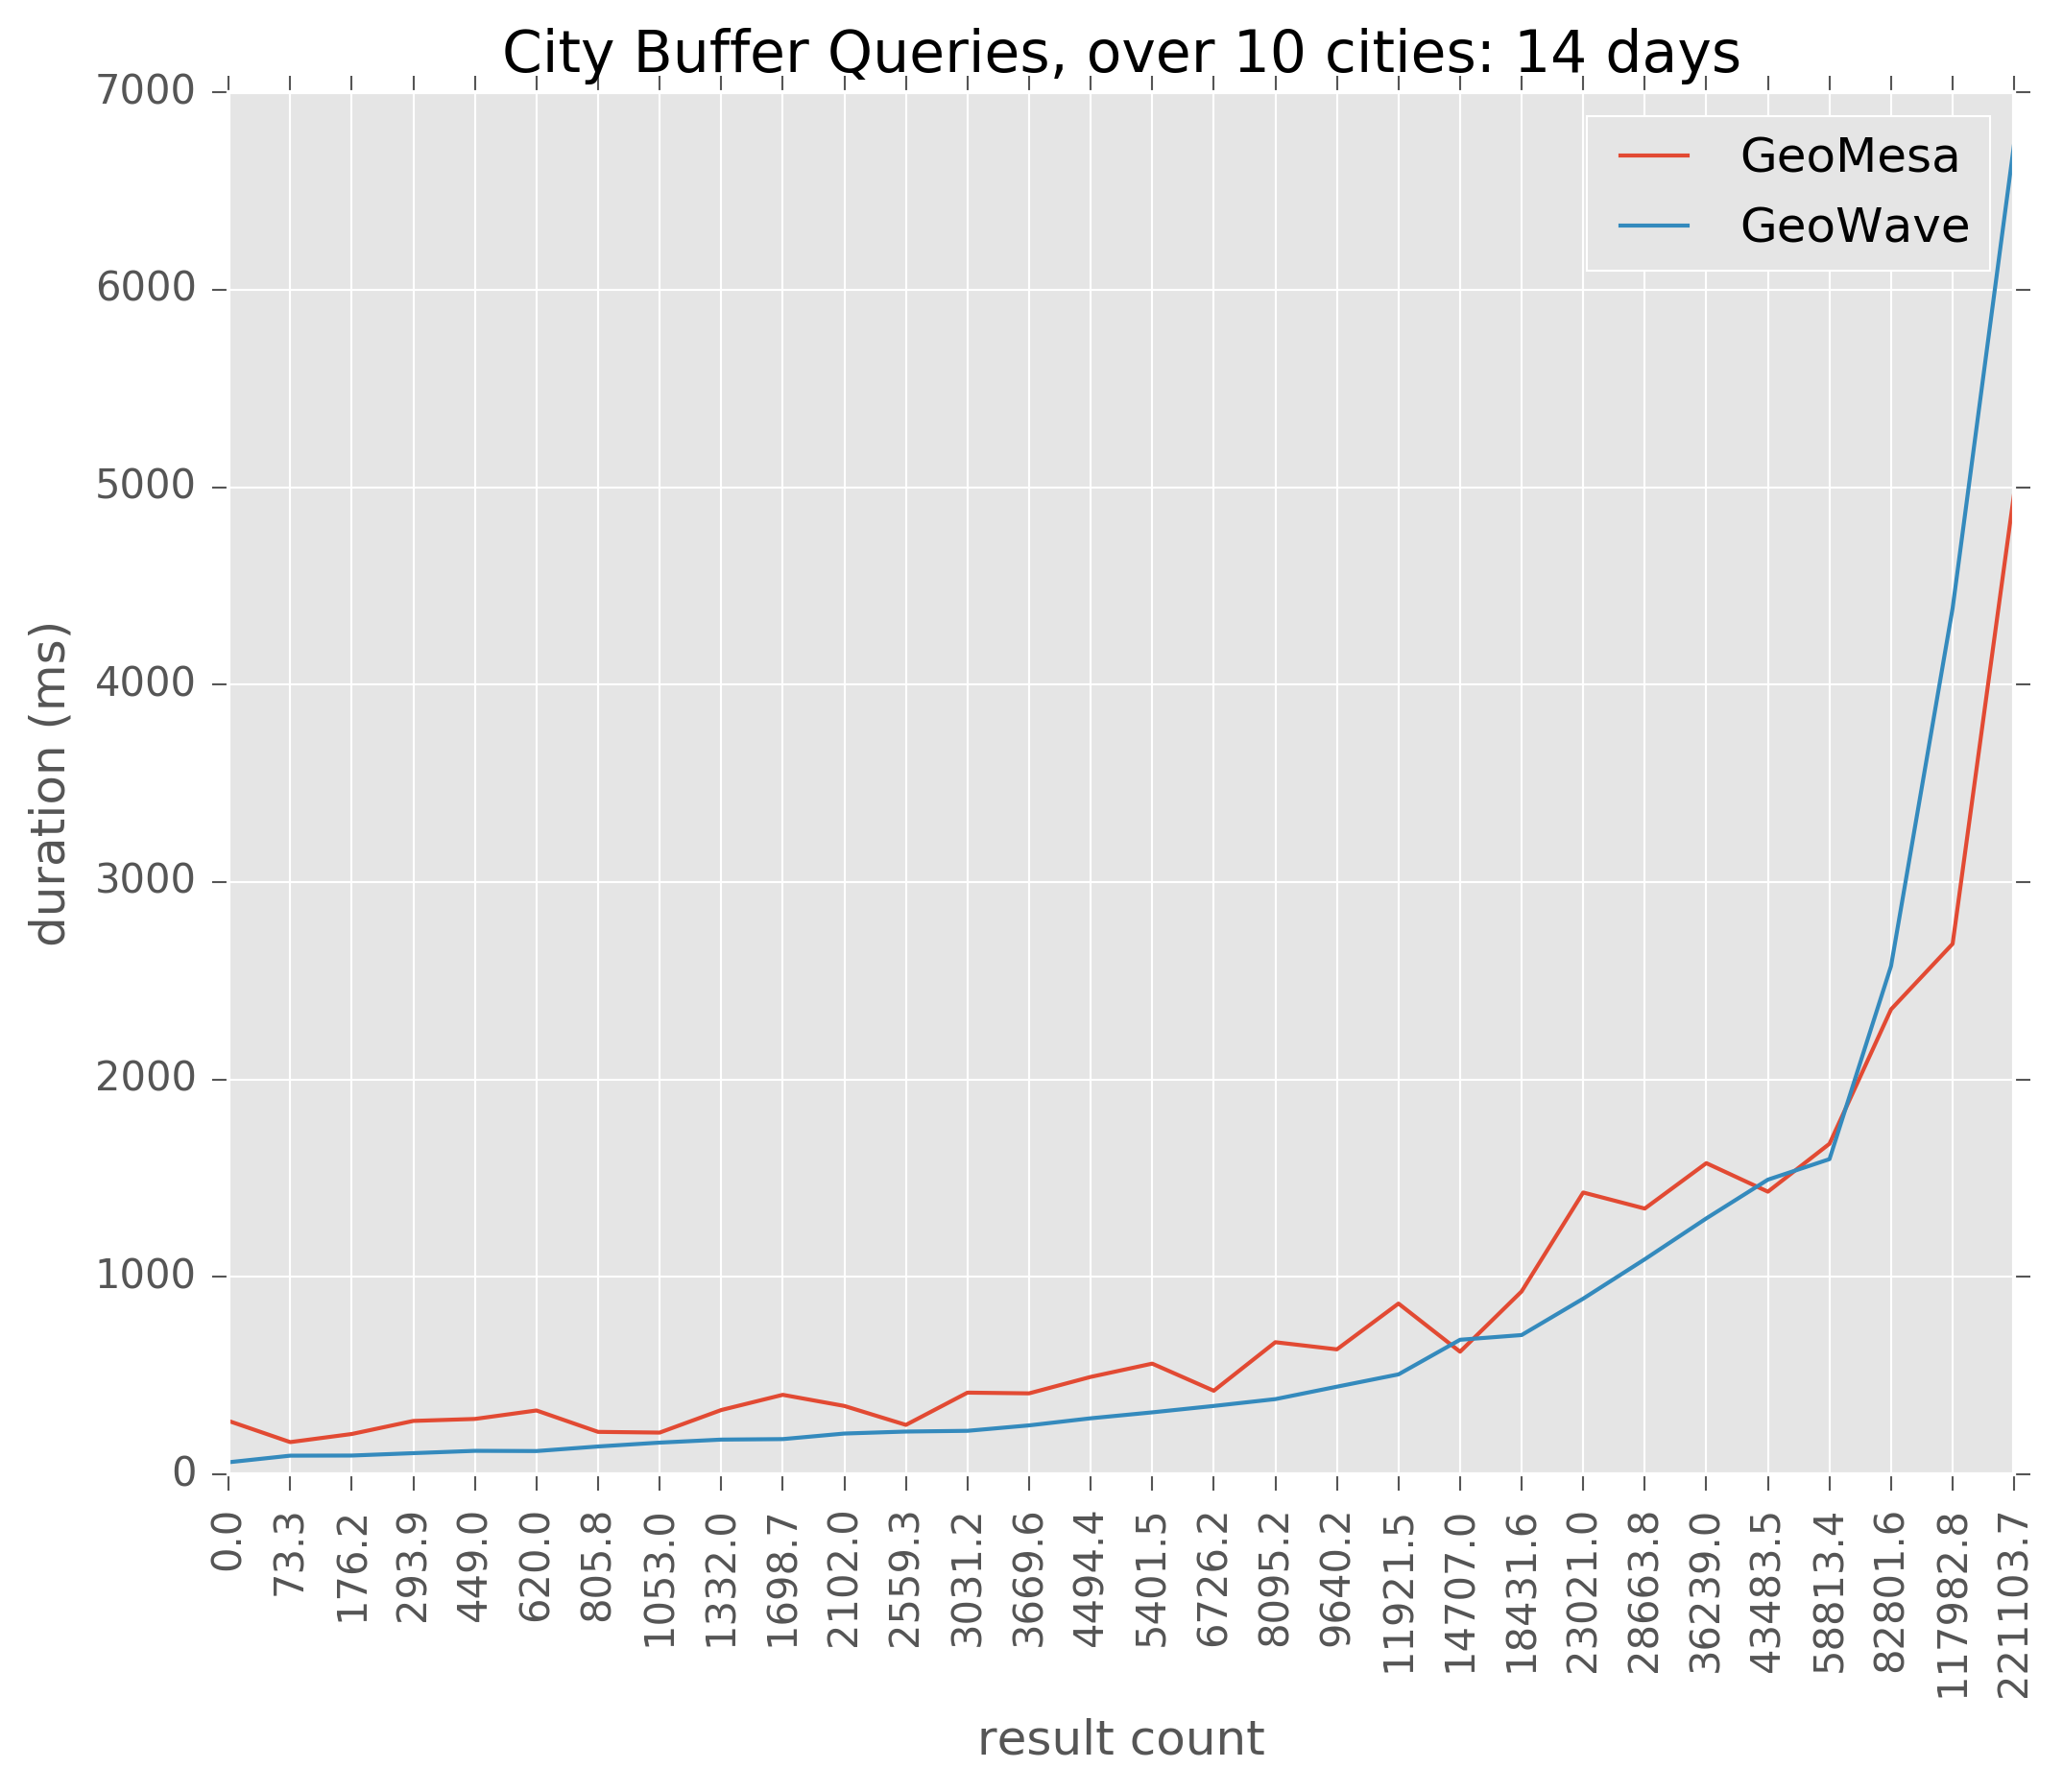
\includegraphics[width=0.60\textwidth]{../docs/img/gdelt/014-days-default.png}
  \caption{Durations over result counts, default indexes, all queries of 14 days.}
  \label{durationresultall14}
\end{figure}

We see here that again GeoMesa appears to be slower than GeoWave,
until a certain result count is reached,
after which it performs better.

If we take a look at the next graph, another pattern emerges.
Figure \ref{durationresultall168} moves the temporal bounds of the query to $168$ days.

\begin{figure}[h!tb]
  \centering
  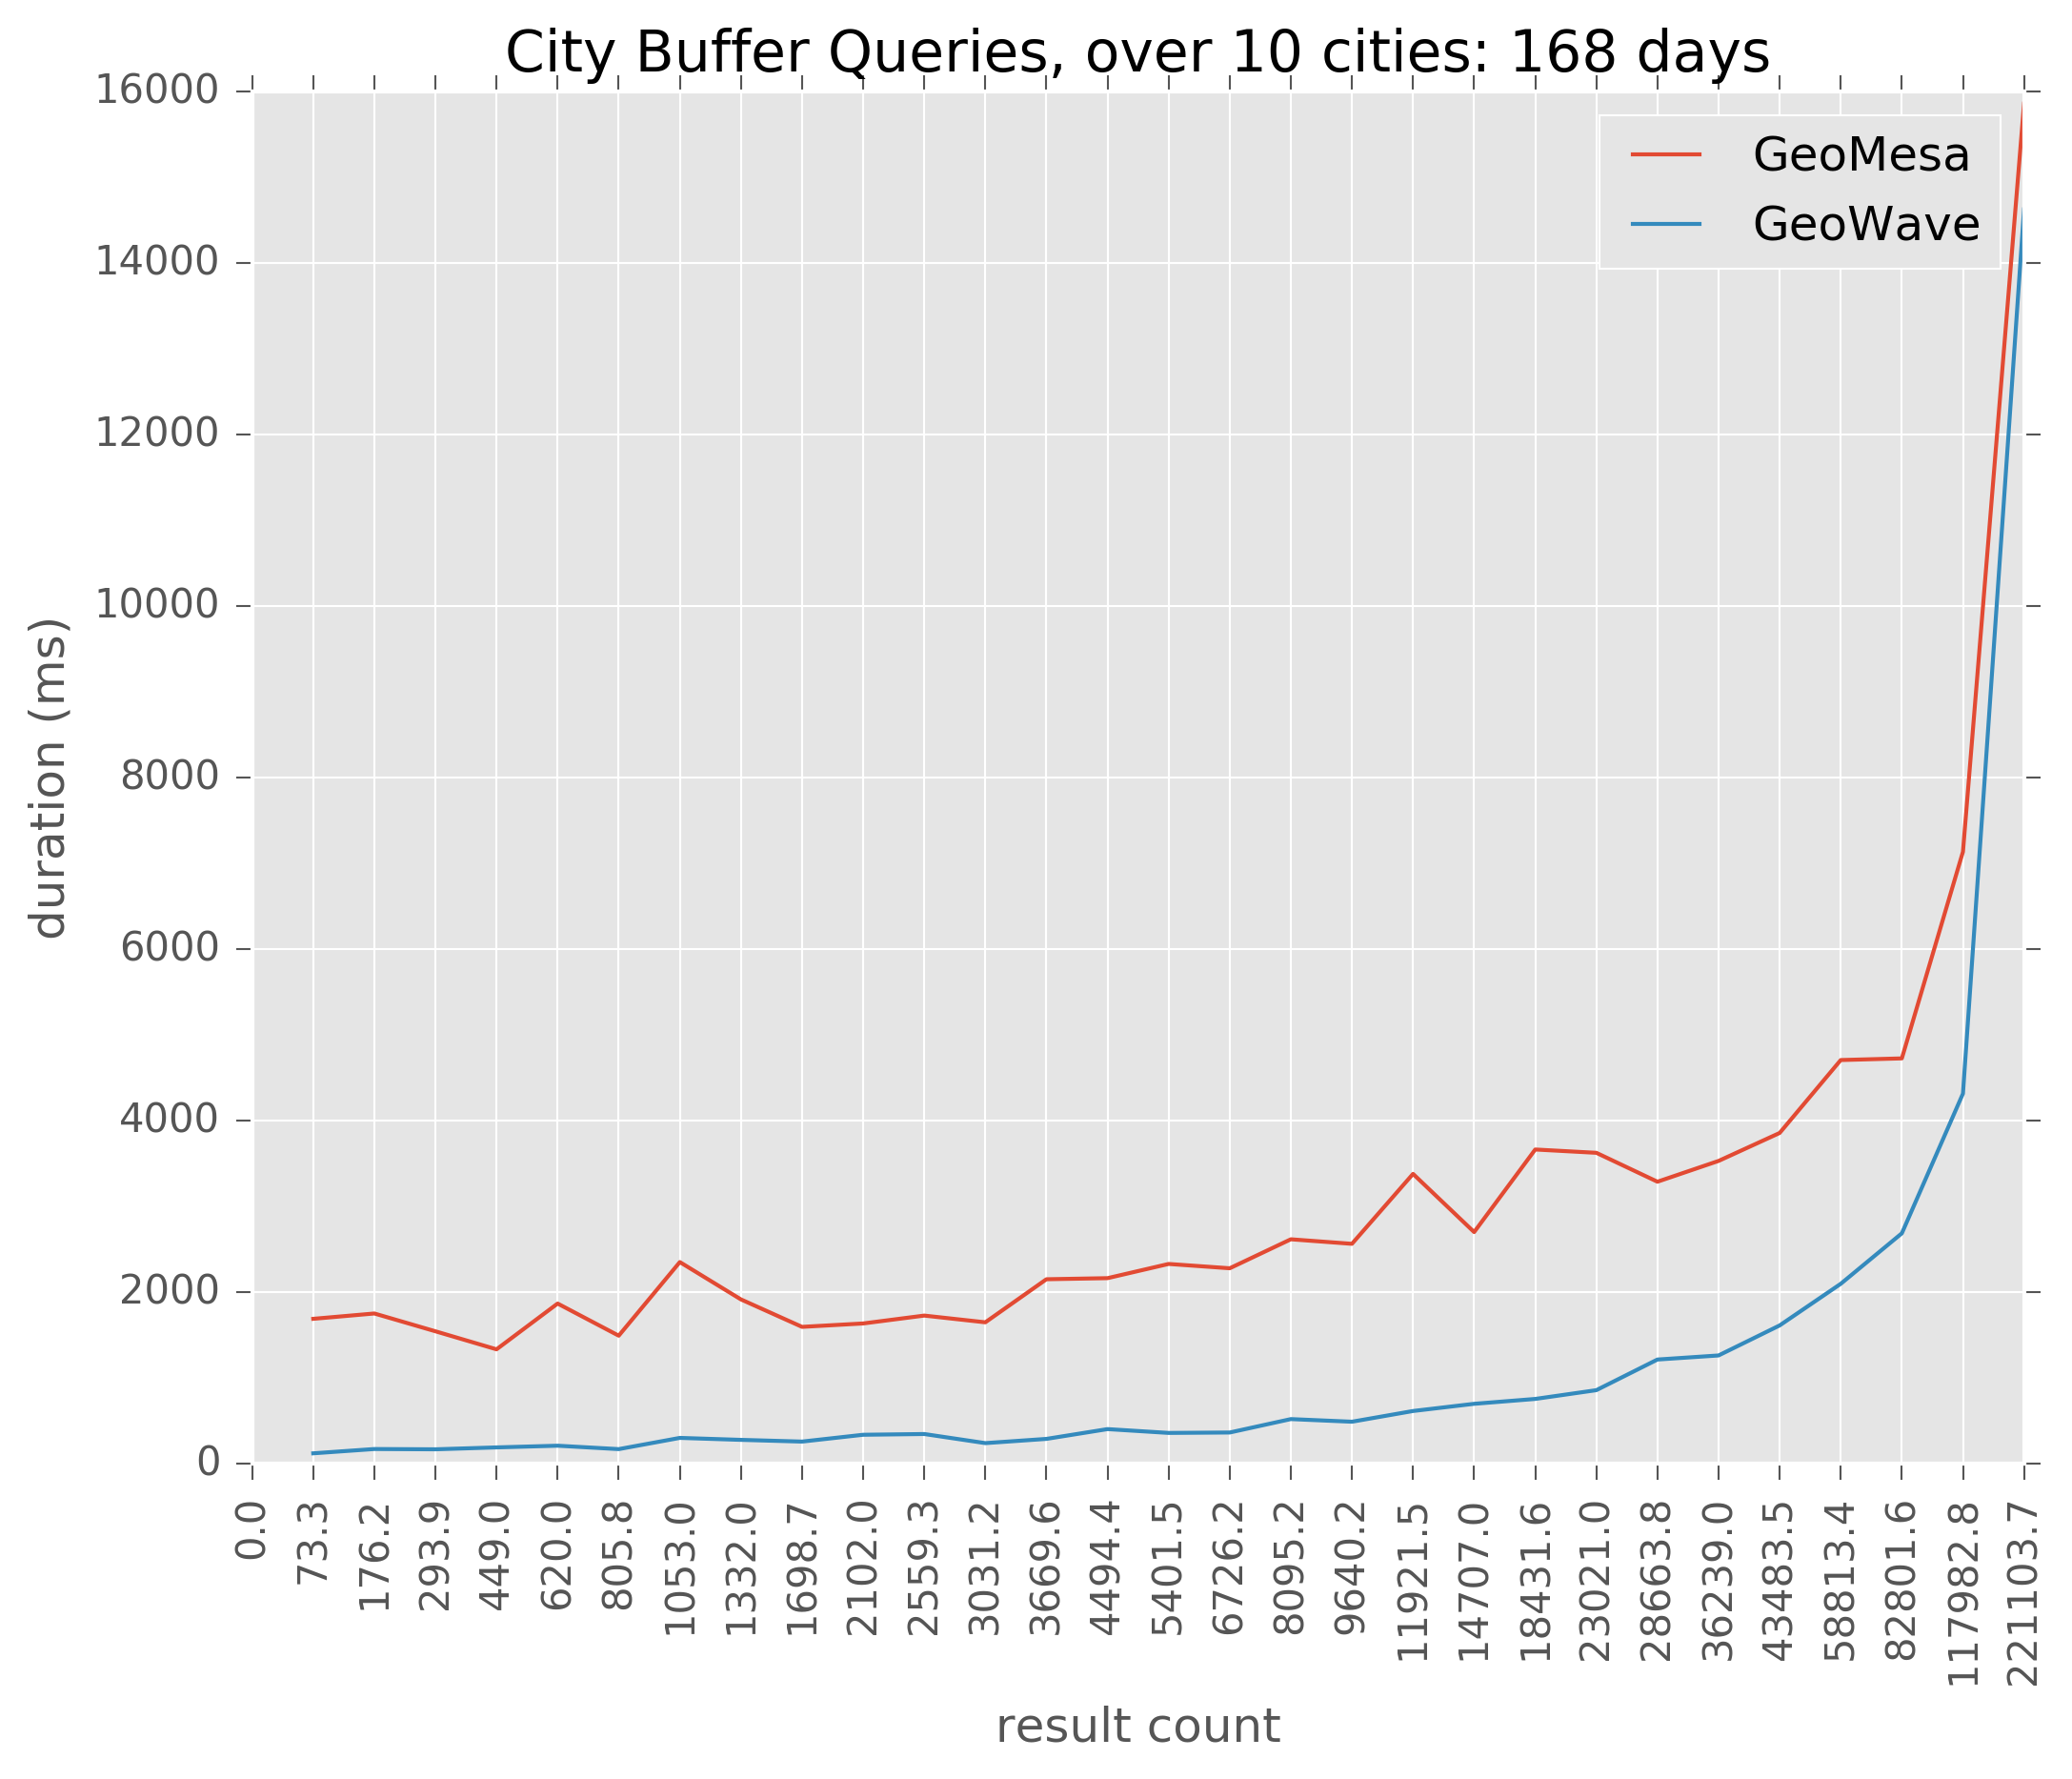
\includegraphics[width=0.60\textwidth]{../docs/img/gdelt/168-days-default.png}
  \caption{Durations over result counts, default indexes, all queries of $168$ days.}
  \label{durationresultall168}
\end{figure}

We see GeoMesa performing worse than the $14$ day case.
In this case it actually never crosses the threshold where it starts outperforming GeoWave based on result count
(according to this technique of averaging result count).

\subsubsection{Index configurations}

We hypothesized that some of the timing differences we were seeing here was because of differences in the configuration
of their indexing mechanisms. As described in the section comparing the index configurations, the default periodicity
for GeoMesa is one week, while in GeoWave it is one year. Also, GeoWave does not shard it's data by default.
To find out how this configuration might be affecting the timing results, we tested with both systems set
to having the following configuration:

\begin{itemize}
\item Both systems configured to have a periodicity of one month, with default sharding
\item Both systems configured to have a periodicity of one year, with default sharding
\item Both systems configured to have a periodicity of one year, with 4 shards being generated by a hashing algorithm
\end{itemize}

We attempted to test a configuration where both systems had a periodicity of one week, but this configuration
produces GeoWave results that were incorrect.

The last configuration in the list above produced improvements in timing results for the City Buffer queries, which we will explore below,
and be referred to as the ``matched'' index configuration.

Figure \ref{matching14} shows the durations of $14$ day queries averages broken into the same result count quartiles.
We can see a marked improvement in GeoMesas results.

\begin{figure}[h!tb]
  \centering
  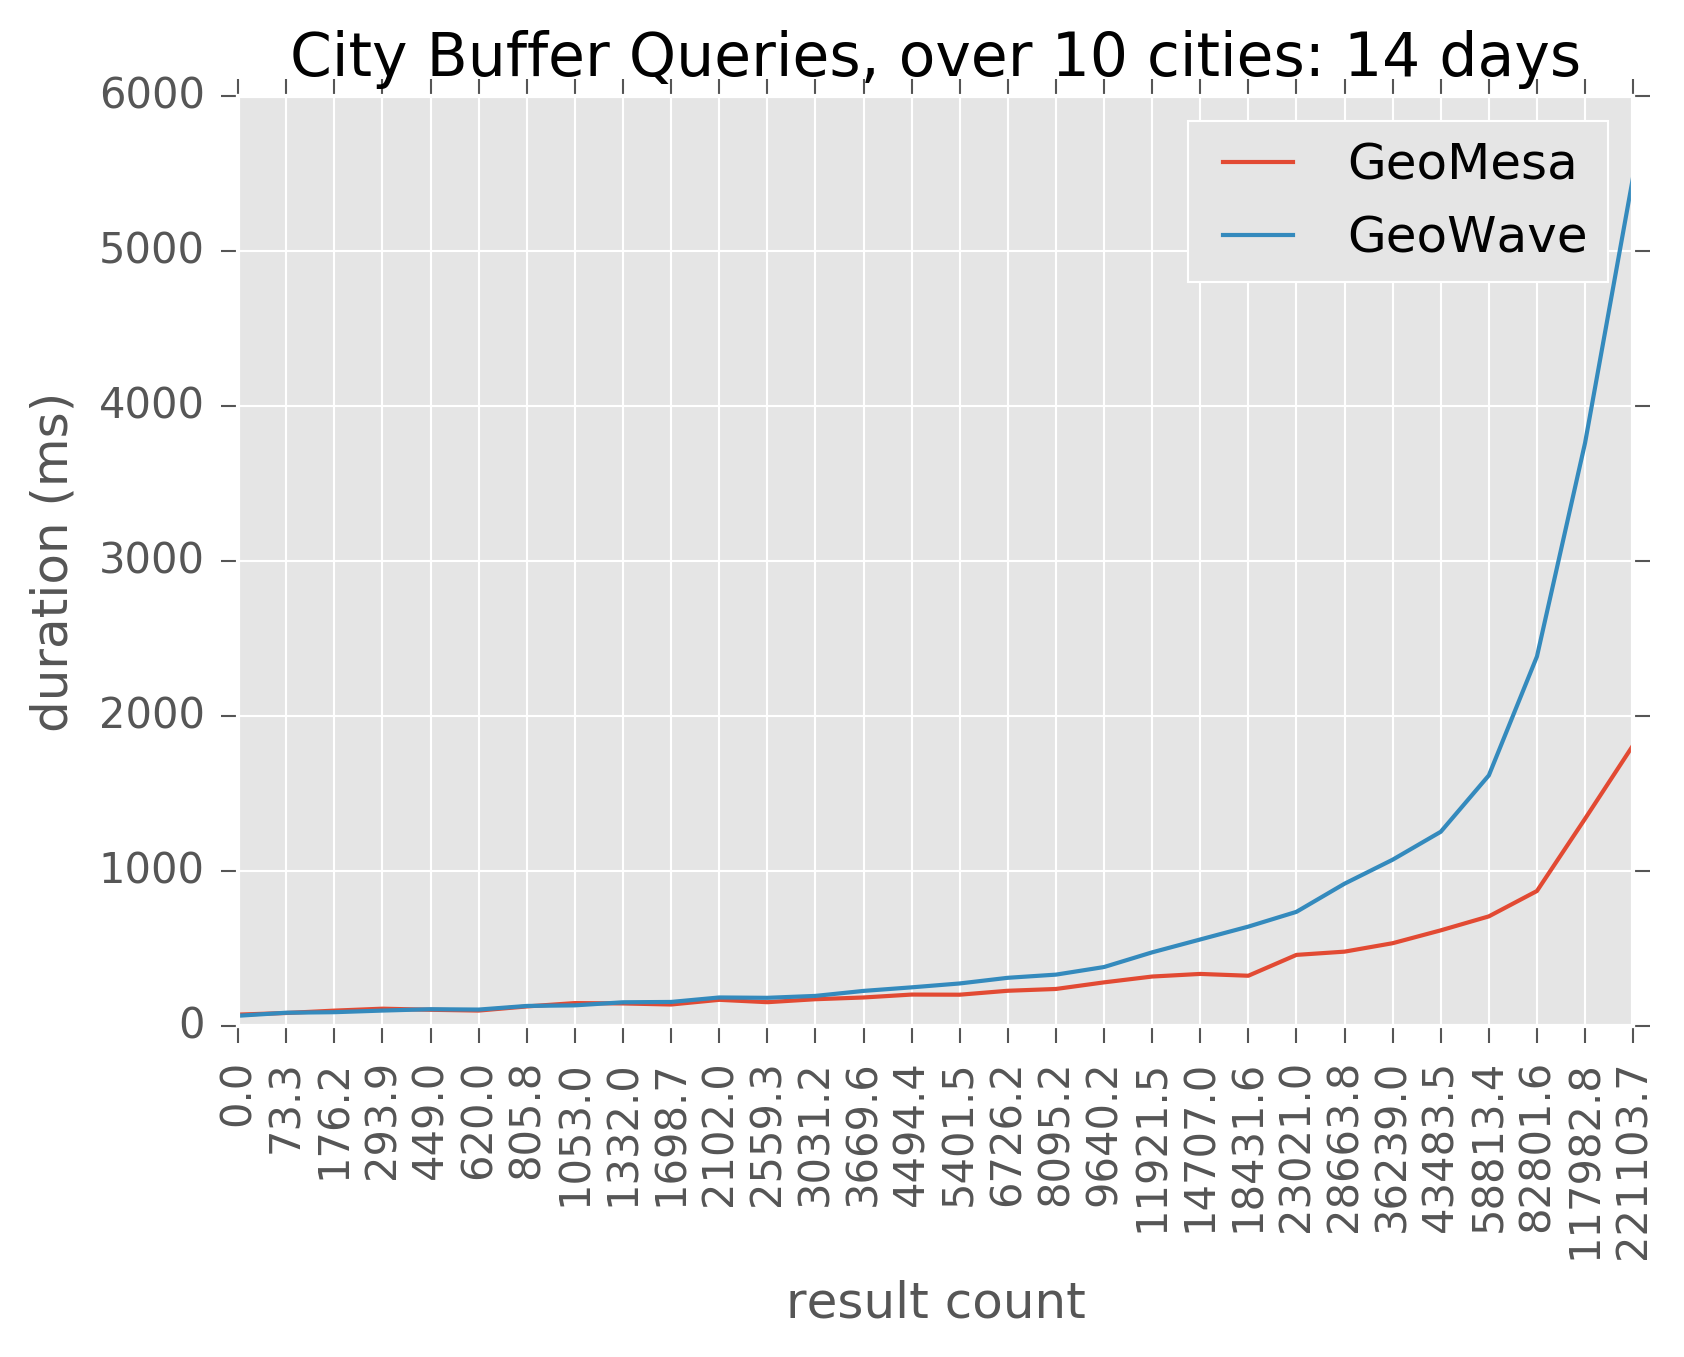
\includegraphics[width=0.60\textwidth]{../docs/img/gdelt/014-days-matching.png}
  \caption{Durations over result counts, matching indexes, all queries of $14$ days.}
  \label{matching14}
\end{figure}

In the case of the $168$ day queries, we see that although there is still a degradation of performance for GeoMesa,
it is not nearly as prominent as it was with the default indexing.
Please see Figure \ref{matching168}.

\begin{figure}[h!tb]
  \centering
  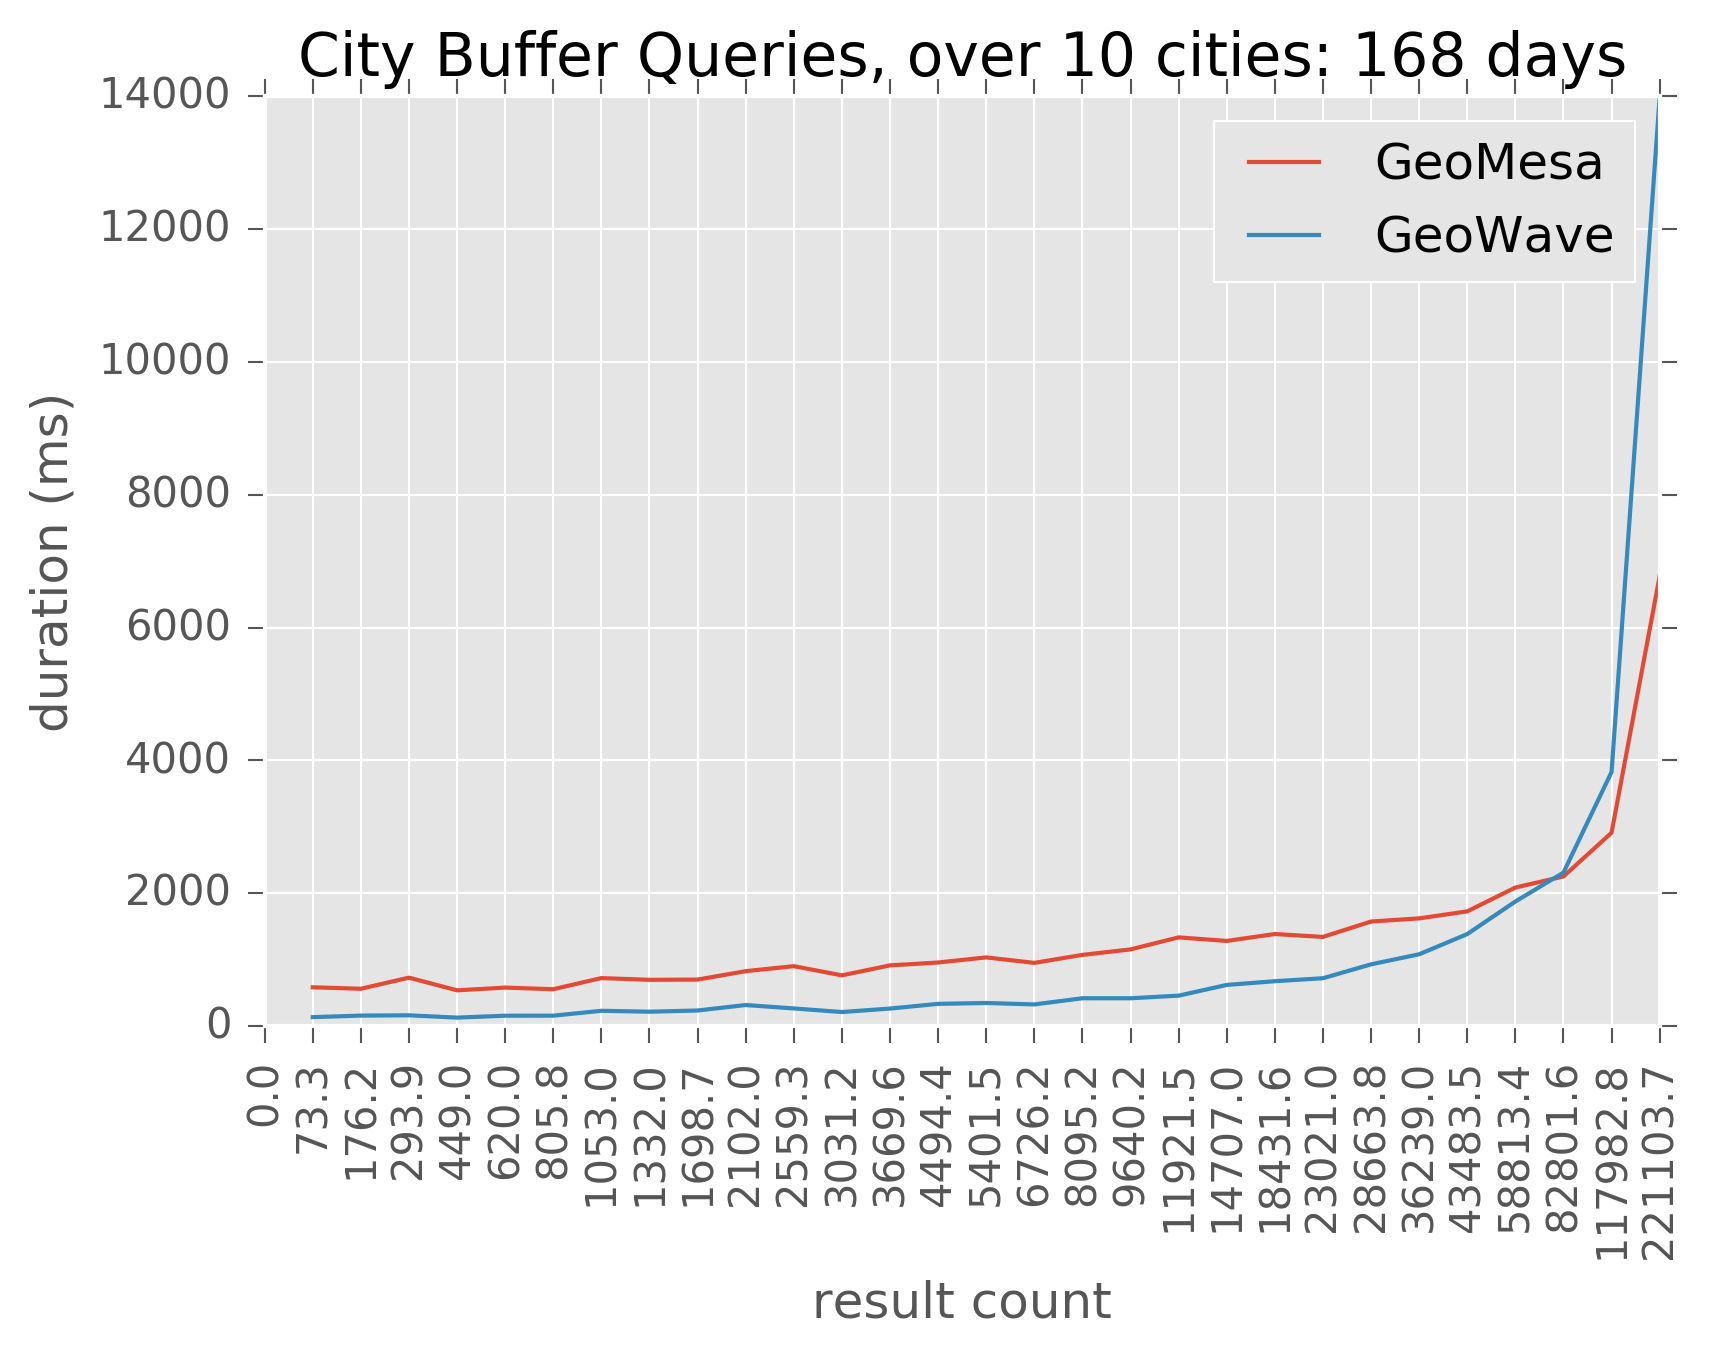
\includegraphics[width=0.60\textwidth]{../docs/img/gdelt/168-days-matching.png}
  \caption{Durations over result counts, matching indexes, all queries of $168$ days.}
  \label{matching168}
\end{figure}

When we look at the overall timings based on result count, we can that GeoMesa seems to be slightly
outperformed by GeoWave until a certain result set size is reached.
Please see Figure \ref{matching}.

\begin{figure}[h!tb]
  \centering
  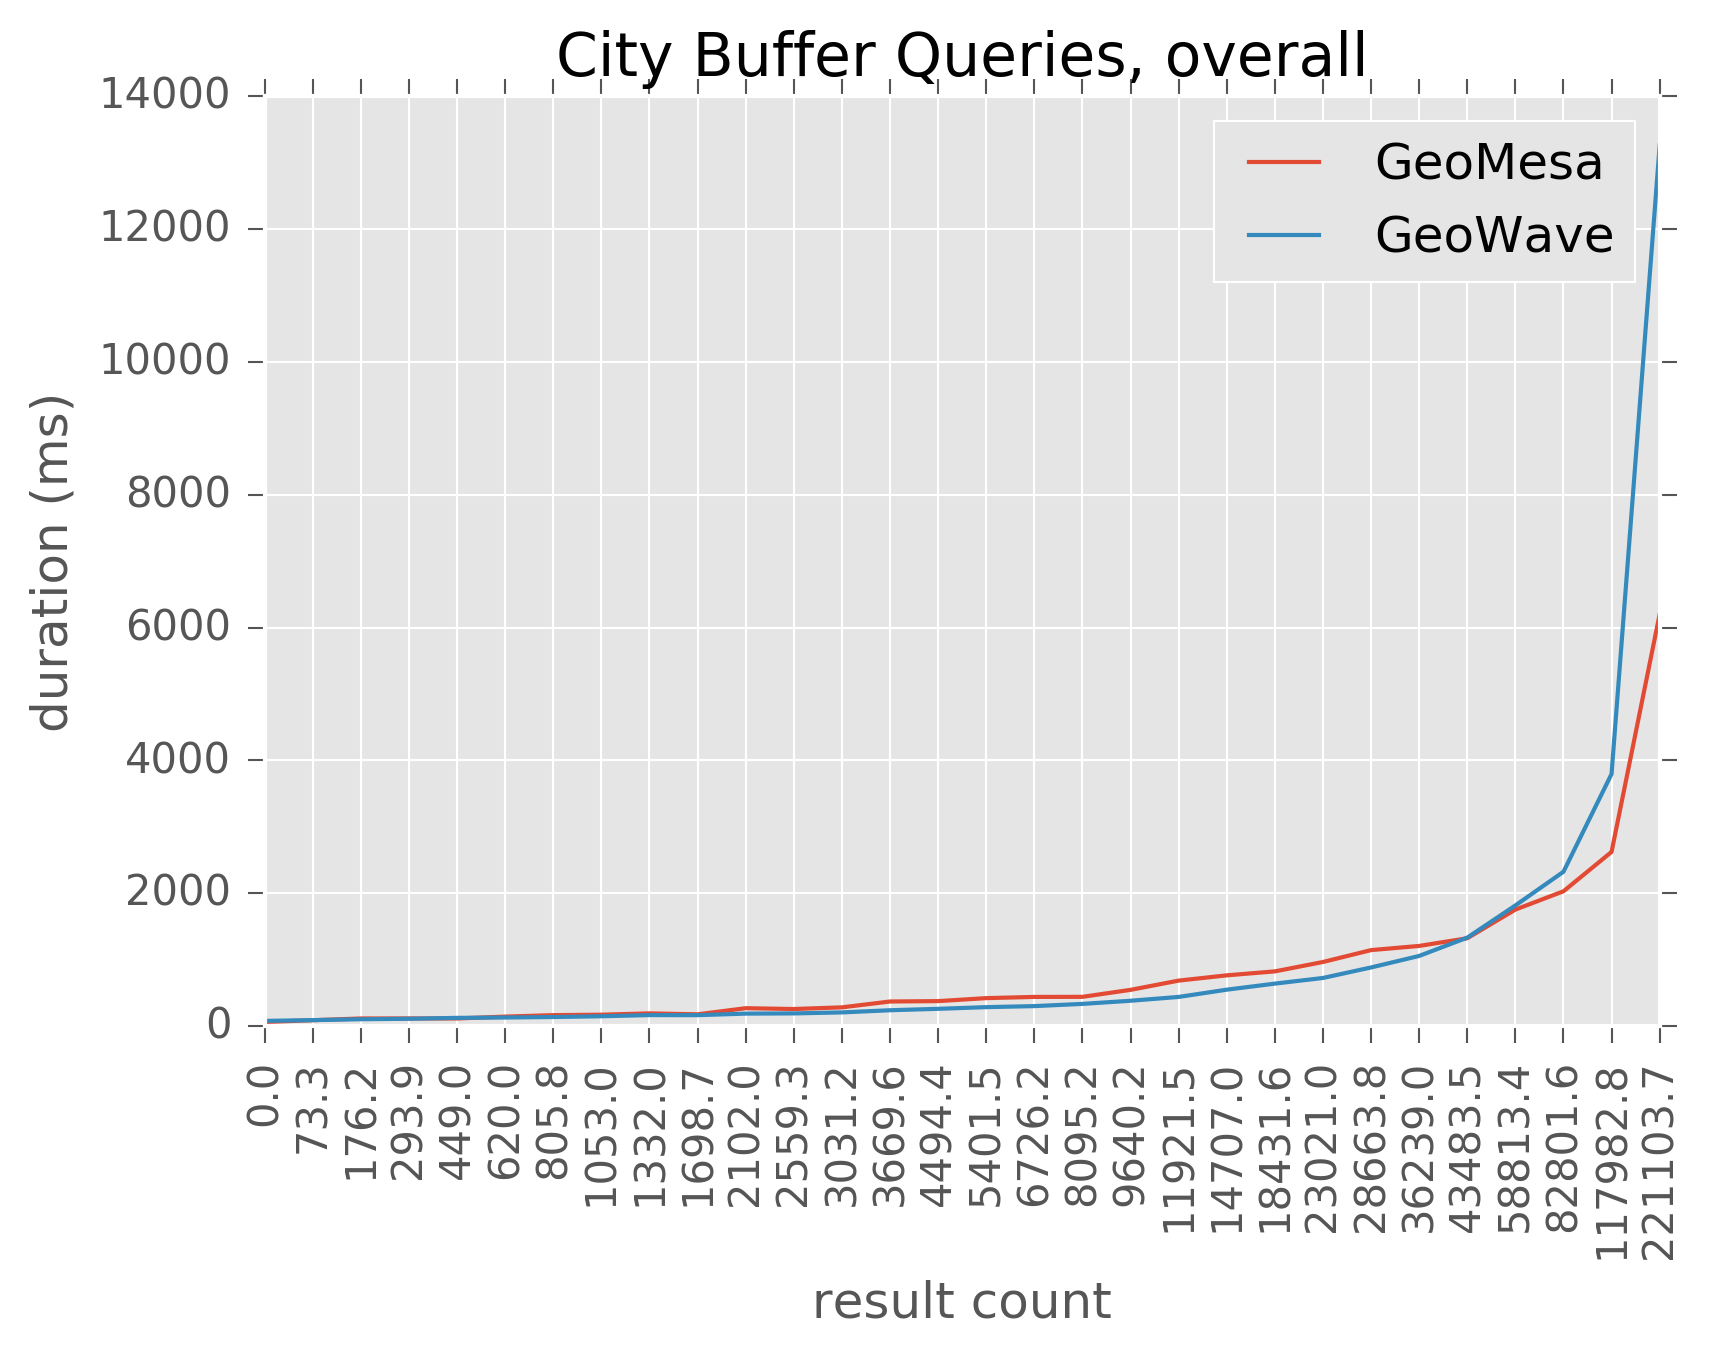
\includegraphics[width=0.60\textwidth]{../docs/img/gdelt/overall-duration-vs-result-matching.png}
  \caption{Durations over result counts, matching, all queries.}
  \label{matching}
\end{figure}

If we focus in on query durations with relatively lower result counts,
and plot GeoMesa and GeoWave results with both the default and the matched index configuration,
we see that both systems improve with the matched index configuration,
and that GeoWave outperforms GeoMesa in this case for both index configurations.
Please see Figure \ref{matchingclamp20}.

%% <!-- ![Durations over result counts, matching, all queries, clamp 20](img/gdelt/overall-duration-vs-result-matching-cap-20.png) -->

\begin{figure}[h!tb]
  \centering
  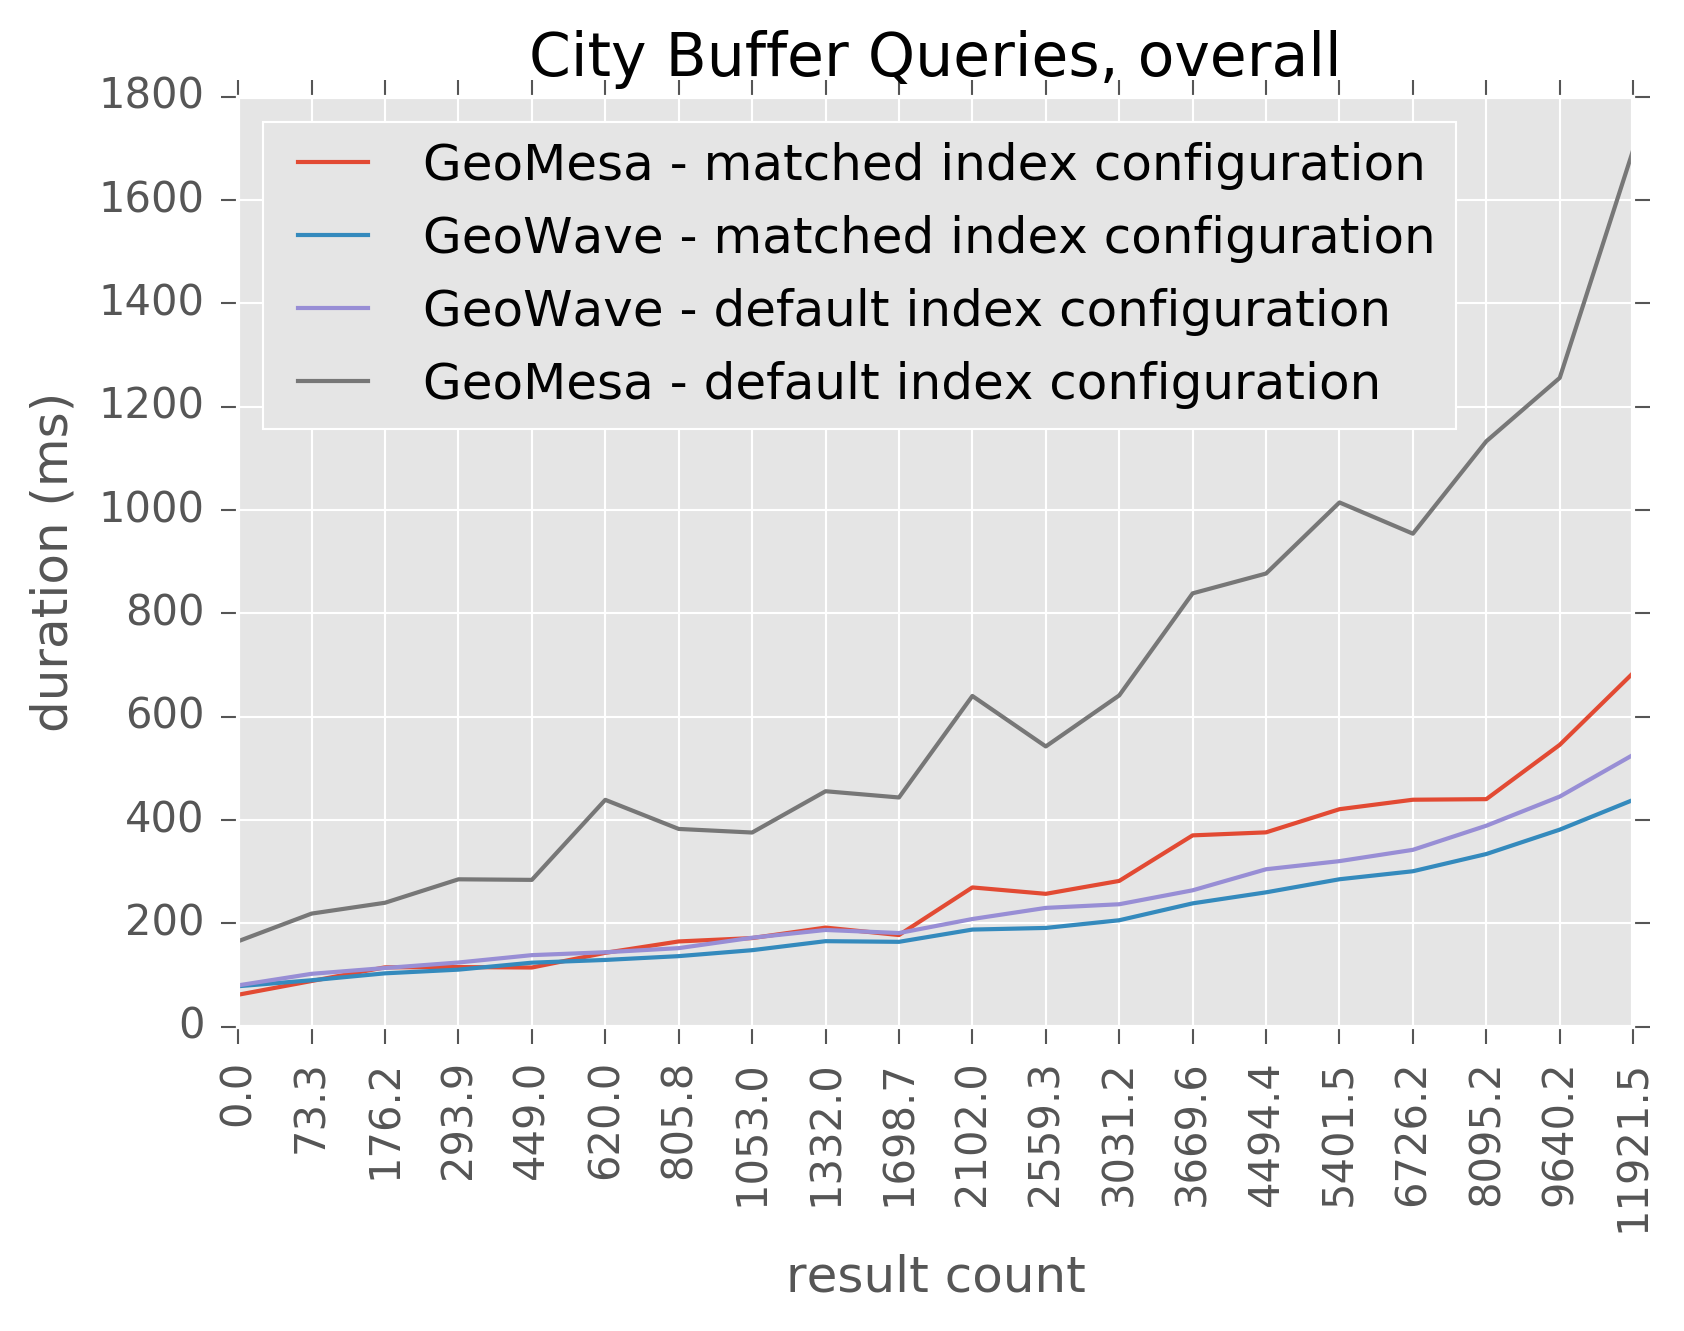
\includegraphics[width=0.60\textwidth]{../docs/img/gdelt/overall-duration-vs-result-both-cap-20.png}
  \caption{Durations over result counts, matching, all queries, clamp $20$.}
  \label{matchingclamp20}
\end{figure}

If we only look at queries with time bounds that are less than 30 days, we see the GeoMesa matched index configuration
performing the best out of that group.
Please see Figure \ref{matchinglt3020}.

\begin{figure}[h!tb]
  \centering
  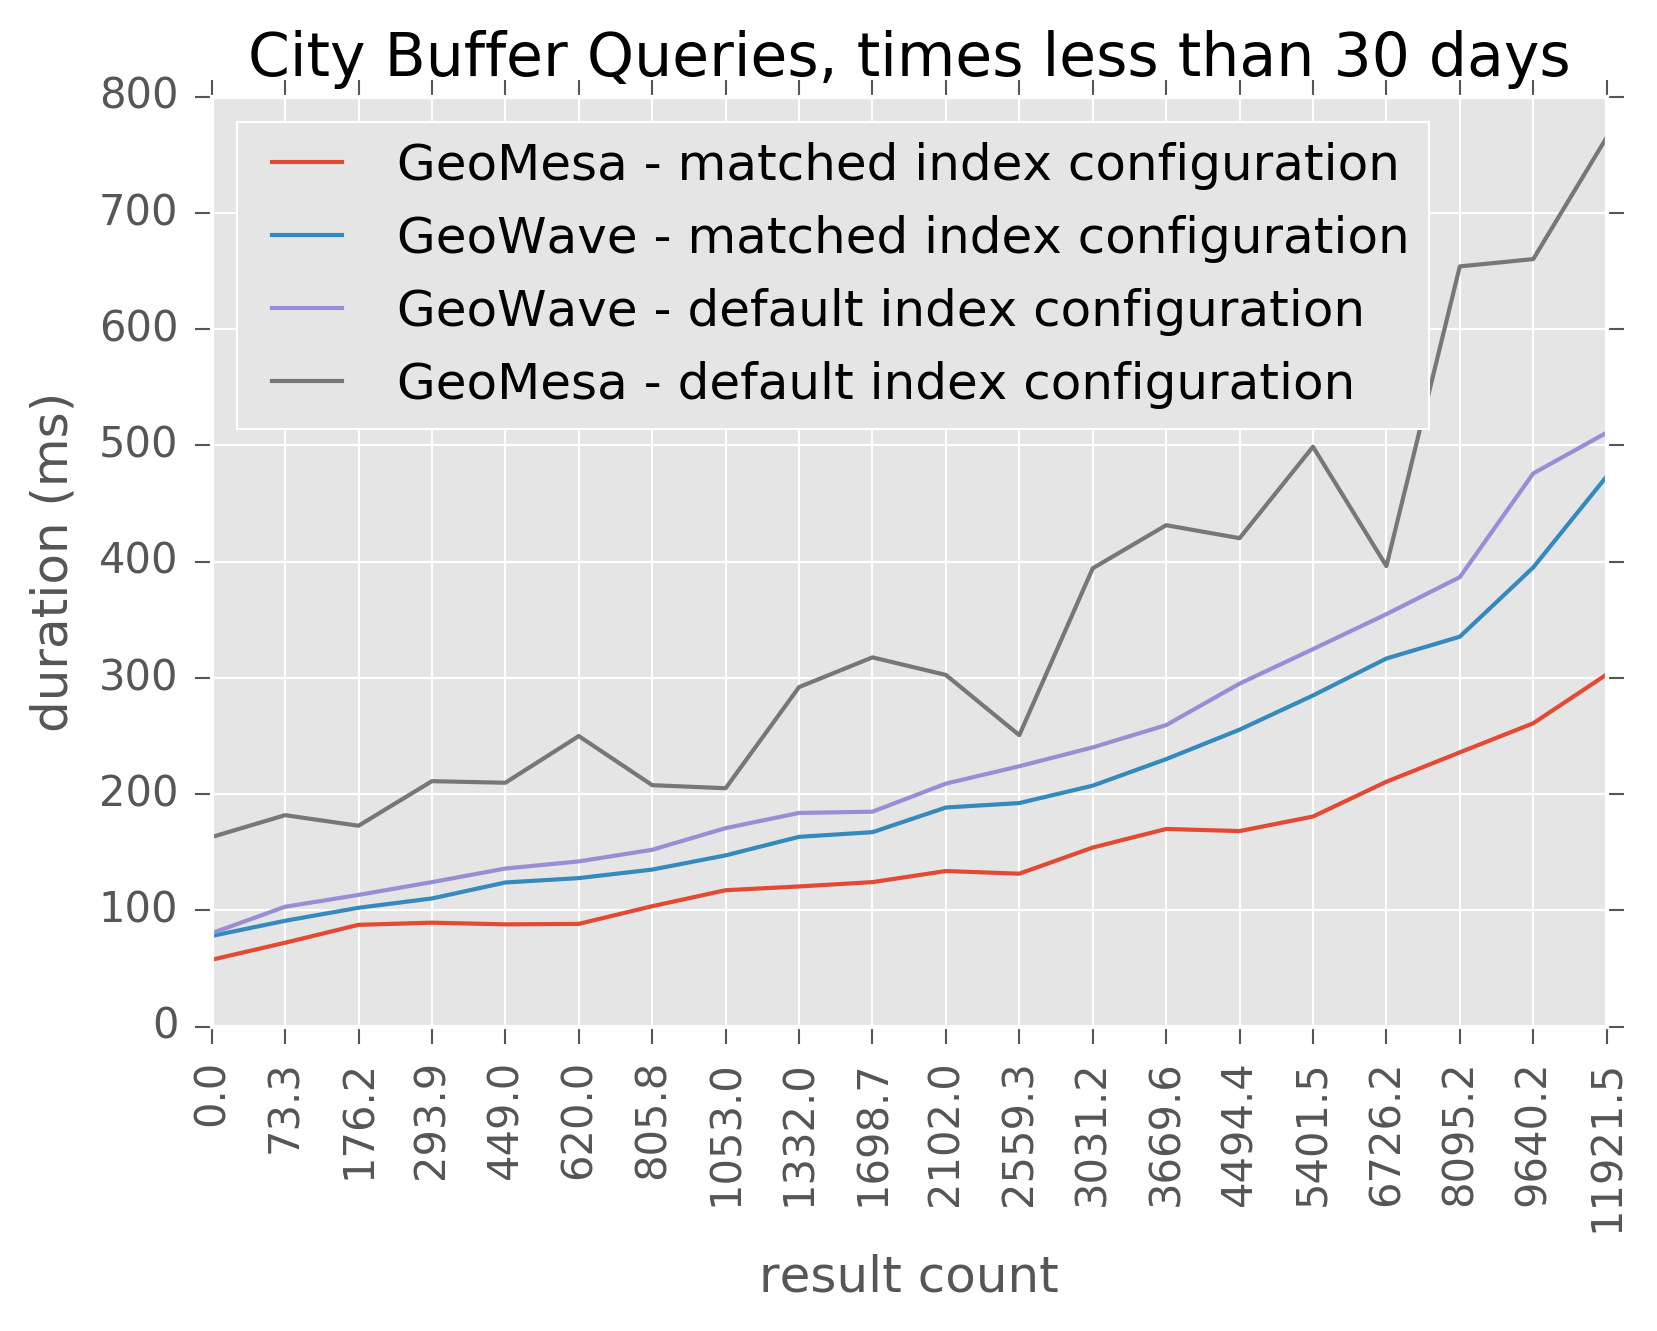
\includegraphics[width=0.60\textwidth]{../docs/img/gdelt/lt-30days-duration-vs-result-both-cap-20.png}
  \caption{Durations over result counts, both, less than $30$ days, clamp $20$.}
  \label{matchinglt3020}
\end{figure}

When we only consider queries over 30 days, we see a more marked advantage of GeoWave performance.
Please see Figure \ref{matchinggt3020}.

\begin{figure}[h!tb]
  \centering
  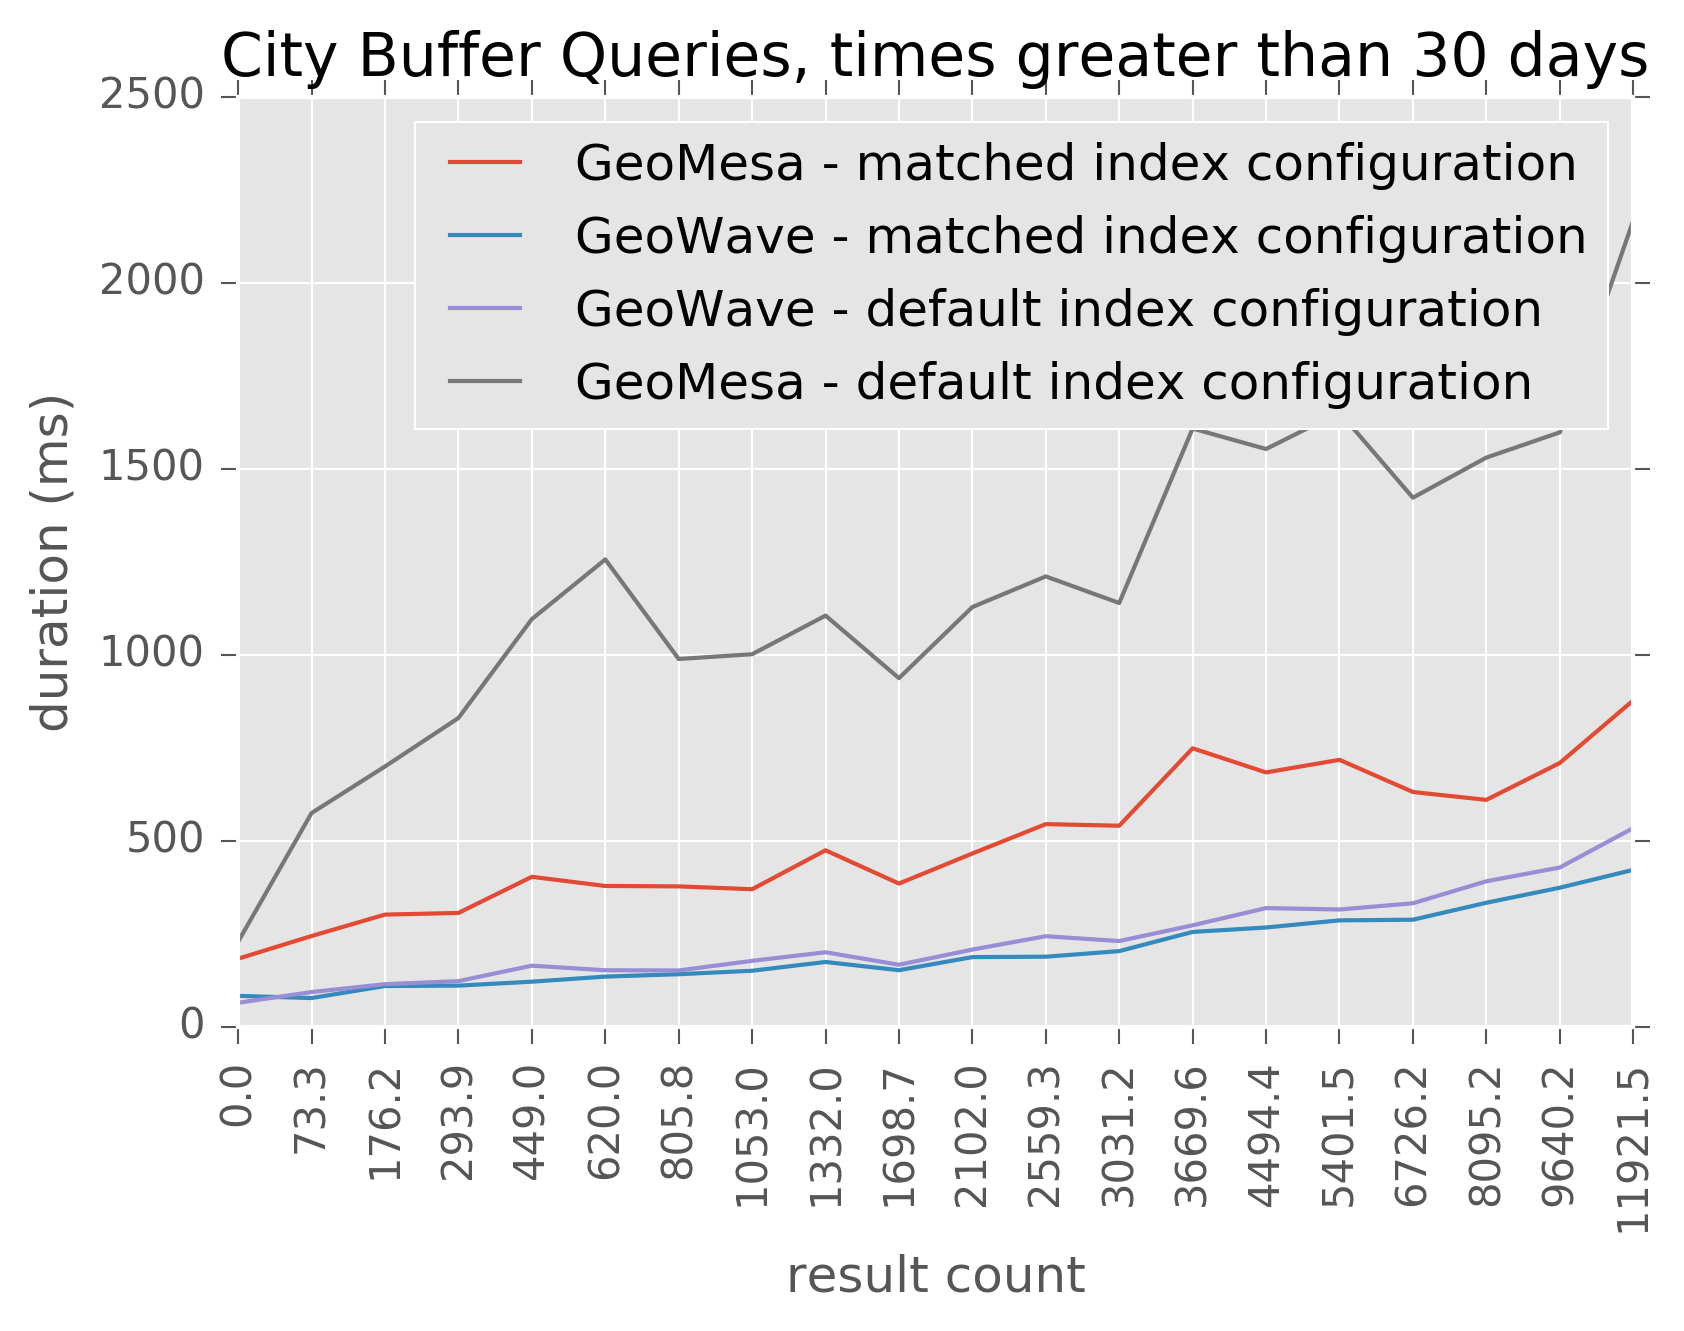
\includegraphics[width=0.60\textwidth]{../docs/img/gdelt/gt-30days-duration-vs-result-both-cap-20.png}
  \caption{Durations over result counts, both, greater than $30$ days, clamp $20$.}
  \label{matchinggt3020}
\end{figure}

%% <!-- ![Durations over result counts, both, less than 30 days](img/gdelt/lt-30days-duration-vs-result-both.png) -->
%% <!-- ![Durations over result counts, both, greater than 30 days](img/gdelt/gt-30days-duration-vs-result-both.png) -->

Here is the duration of queries plotted over the temporal bounds of the query.
We see that GeoMesa performs better for queries with a small time window,
and both GeoMesa and GeoWave show better performance with the matched index configuration.
Please see Figure \ref{durationdaysboth}.

\begin{figure}[h!tb]
  \centering
  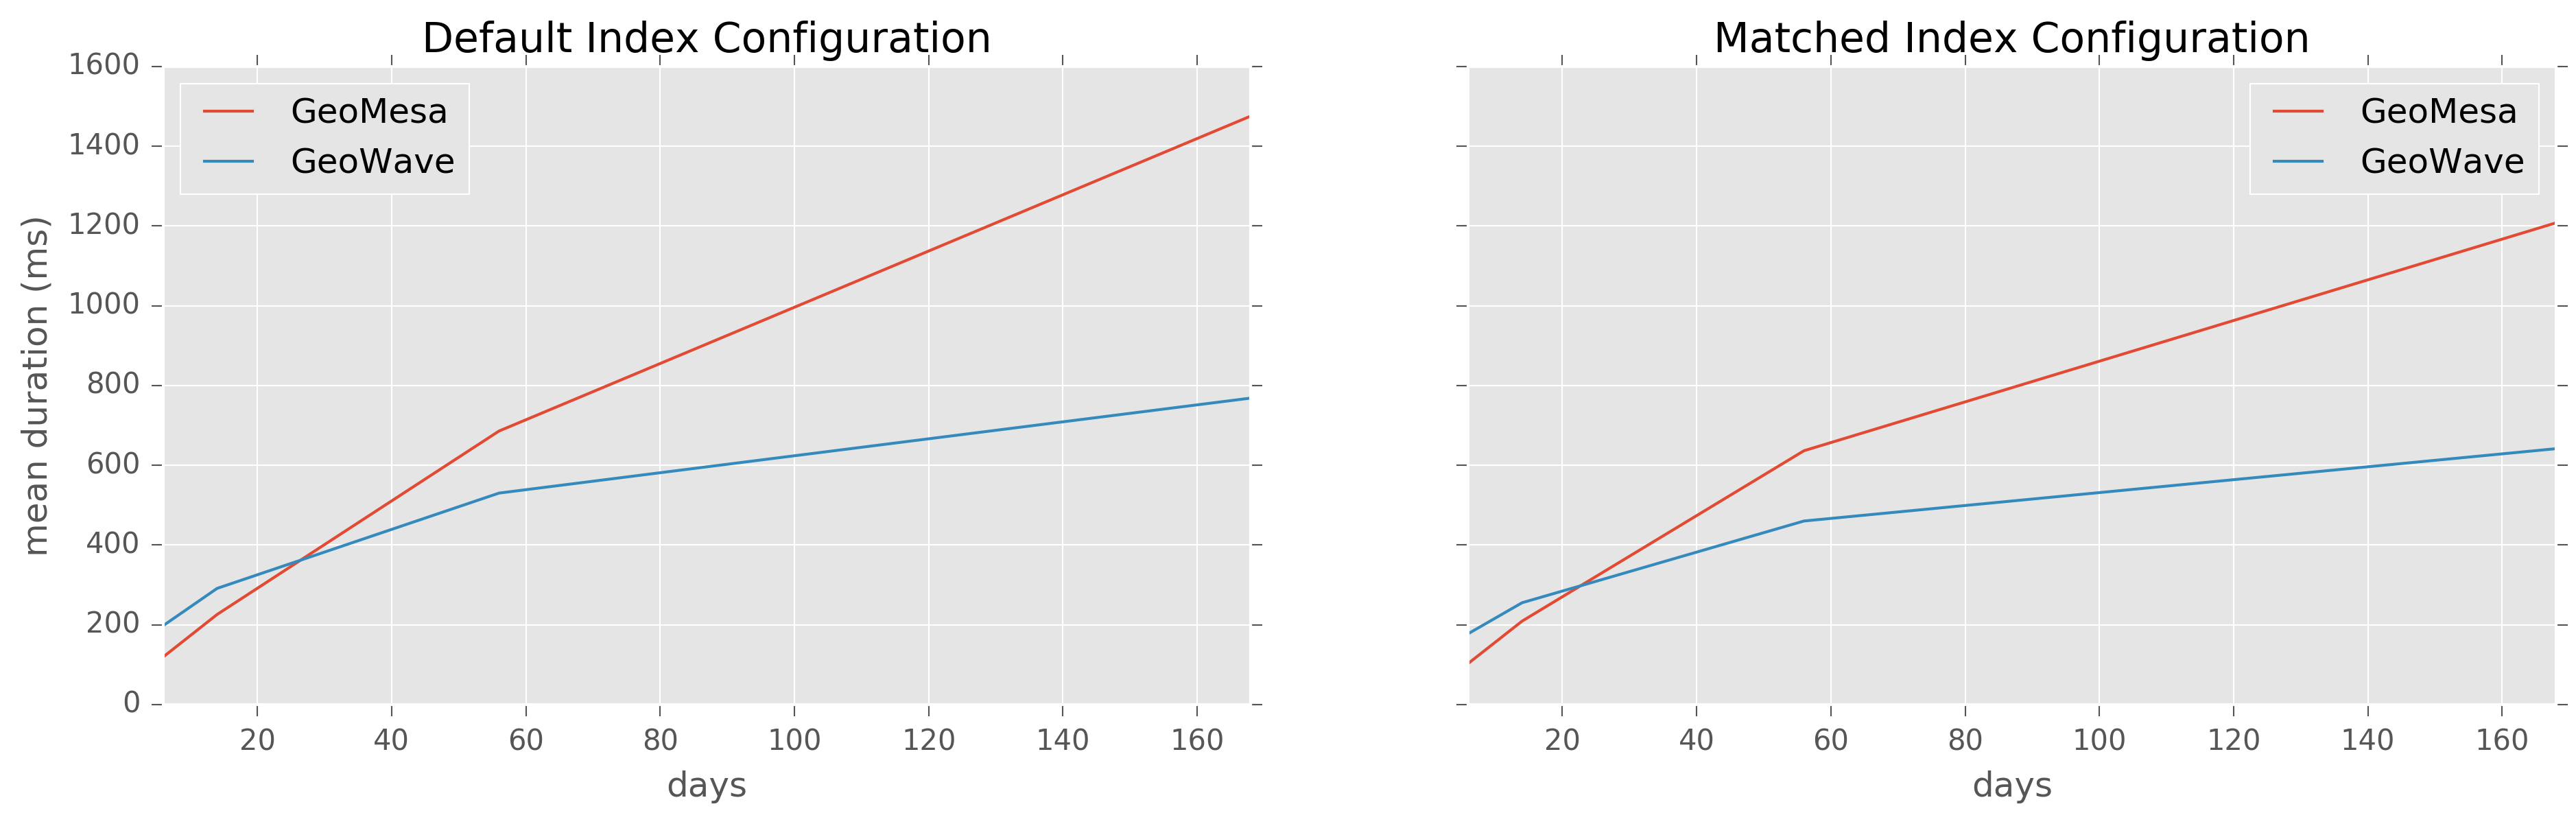
\includegraphics[width=0.60\textwidth]{../docs/img/gdelt/duration-over-days-default-and-matching.png}
  \caption{Durations over days, both.}
  \label{durationdaysboth}
\end{figure}

Looking at the data in another way, we see that the size of the spatial component of the query
(shown in the $x$-axis here in kilometers)
does not have the same threshold-crossing effect as the temporal component does,
and that on average GeoWave outperforms GeoMesa across spatial queries.
Please see Figure \ref{durationsize}.

\begin{figure}[h!tb]
  \centering
  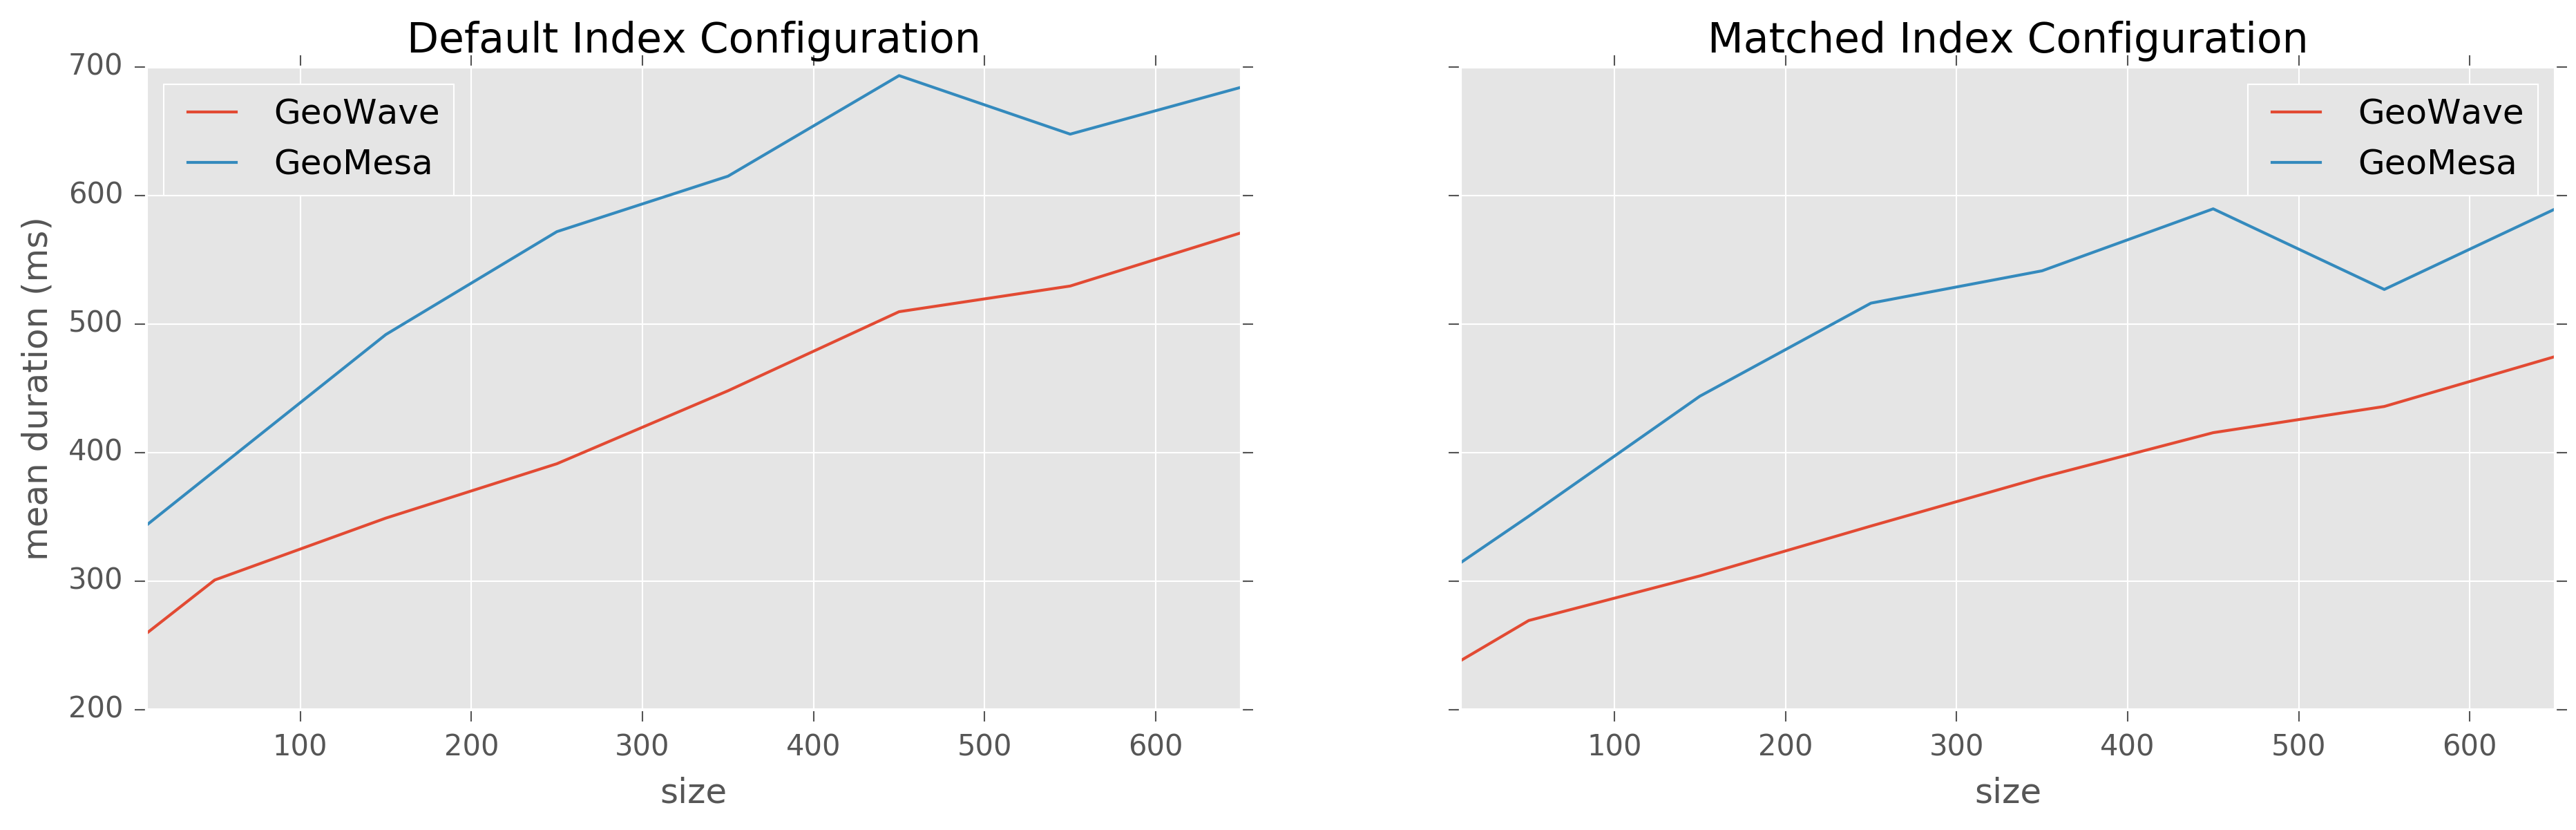
\includegraphics[width=0.60\textwidth]{../docs/img/gdelt/duration-over-size-default-and-matching.png}
  \caption{Durations over days, both.}
  \label{durationsize}
\end{figure}

Finally for the City Buffer tests, we look at how the scatterplot and regression
of durations over result counts changes between the default and the matched index configuration.
Please see Figure \ref{durationresult}.

\begin{figure}[h!tb]
  \centering
  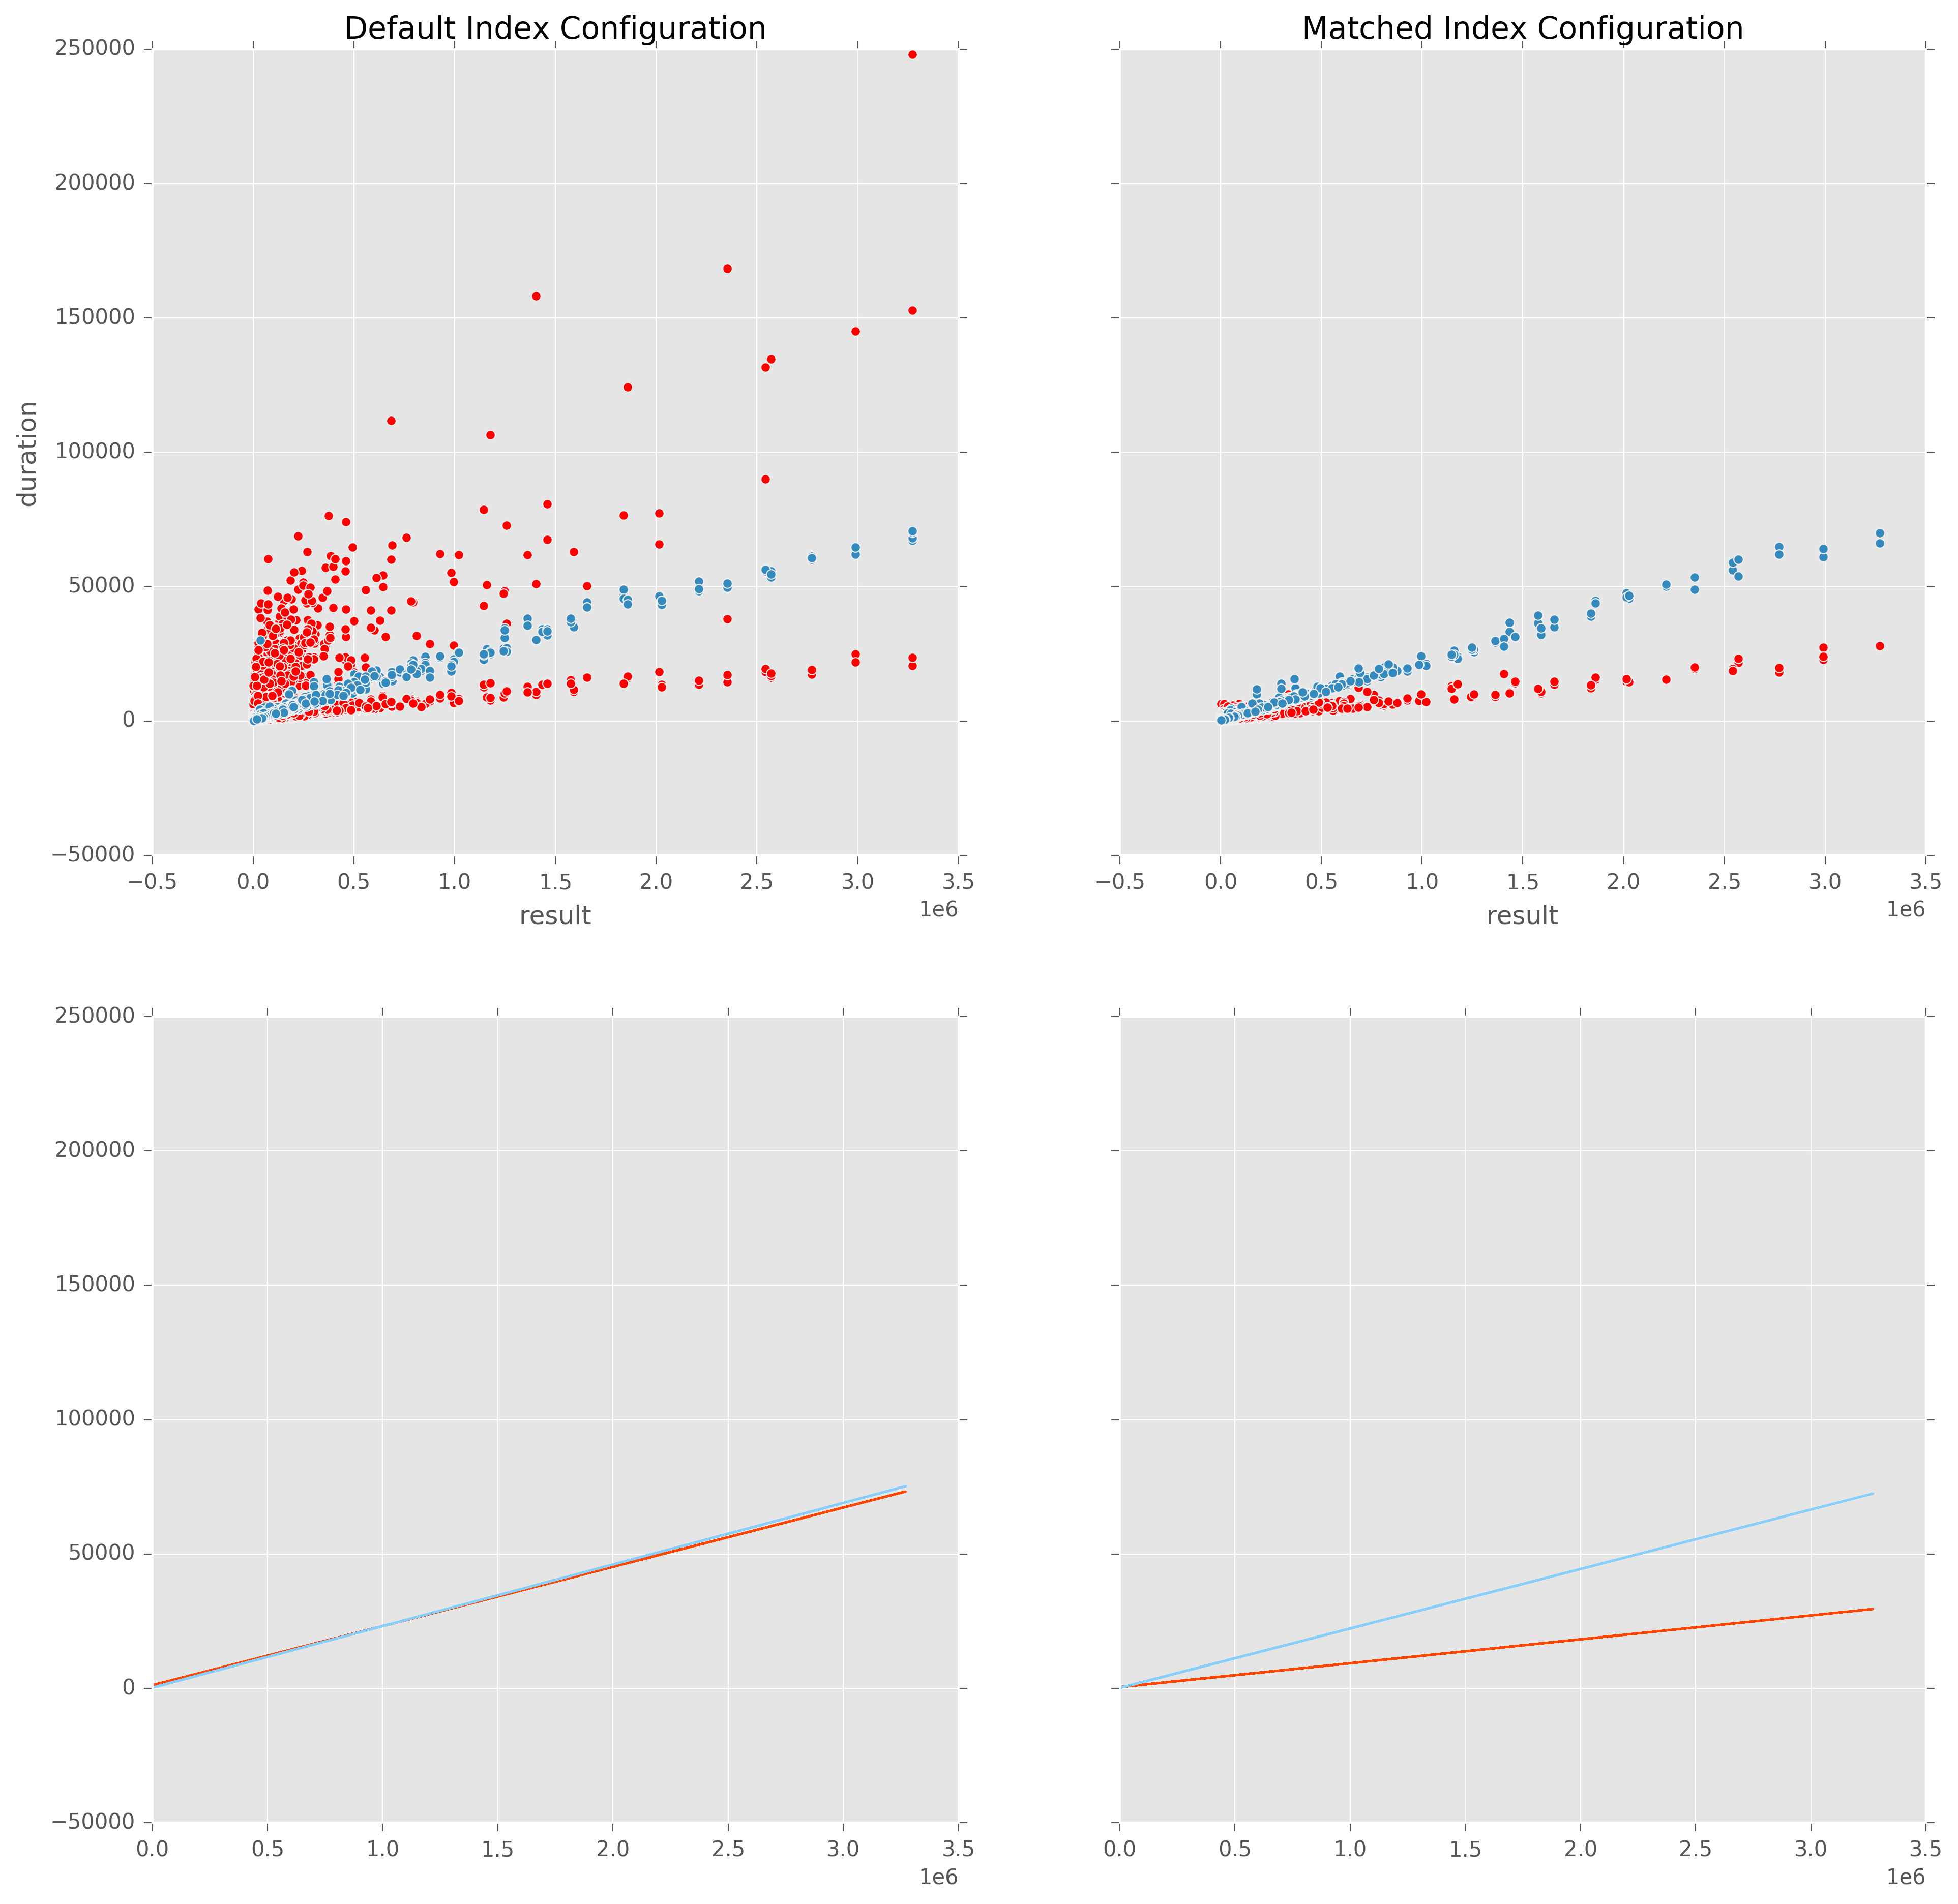
\includegraphics[width=0.60\textwidth]{../docs/img/gdelt/duration-over-result-default-and-matching.png}
  \caption{Durations over result, scatter and regression, both.}
  \label{durationresult}
\end{figure}

\subsubsection{South America}

We queried events within South American countries (Figure \ref{southamerica})
for three weeks of every month of every year from 2000 to 2016.

\begin{figure}[h!tb]
  \centering
  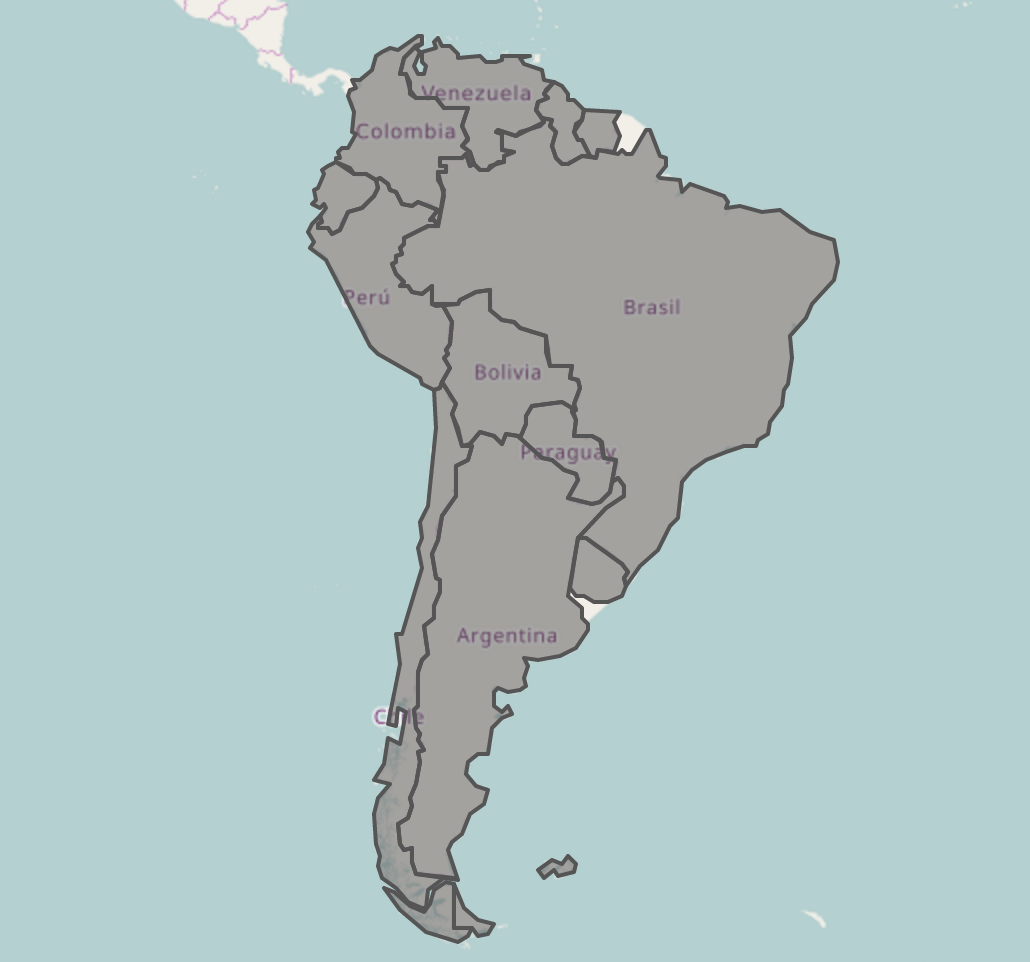
\includegraphics[width=0.60\textwidth]{../docs/img/gdelt/south-america-countries.png}
  \caption{South America.}
  \label{southamerica}
\end{figure}

The results we found for this area of the world were unsurprising,
with the matching index configuration performing better in both systems than the default index configuration,
and the effect of result count having a greater effect on GeoWave performance than GeoMesa.
Figure \ref{sadurations} is a chart is of the duration of query execution over result size, with outliers removed.

\begin{figure}[h!tb]
  \centering
  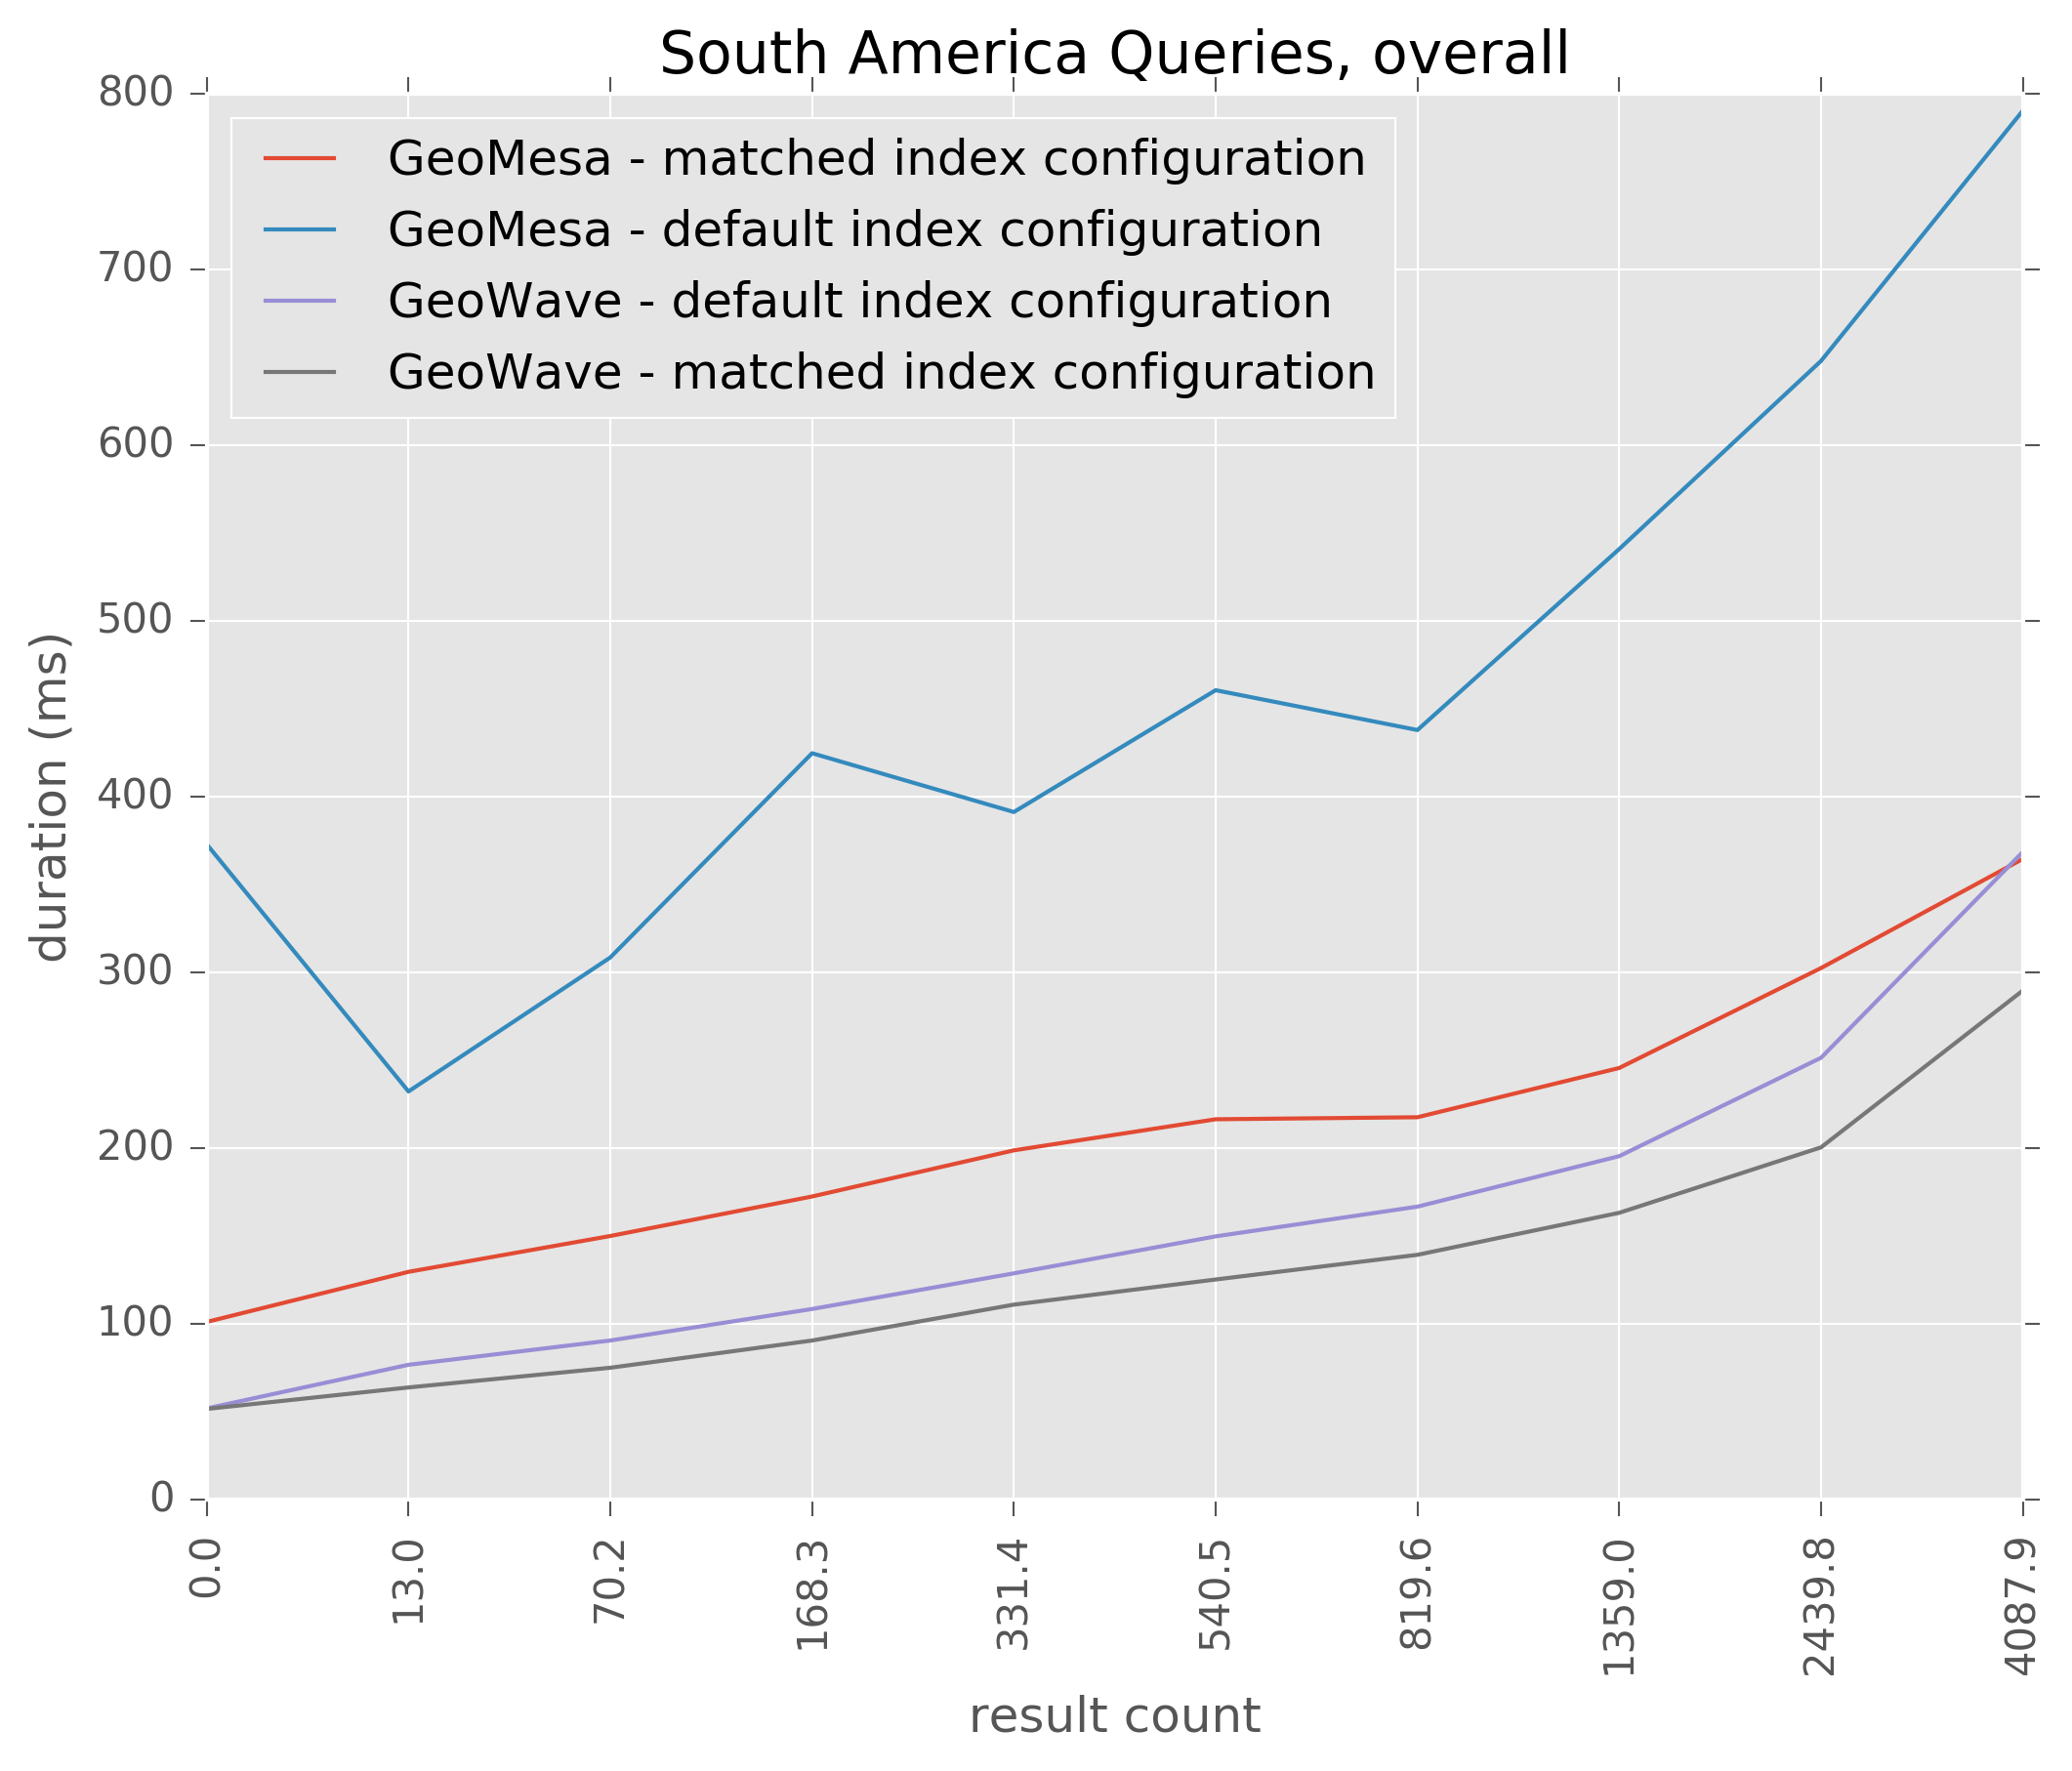
\includegraphics[width=0.60\textwidth]{../docs/img/gdelt/sa-overall-duration-vs-result-both.png}
  \caption{Durations over result counts, both, all queries.}
  \label{sadurations}
\end{figure}


\subsection{Synthesized Tracks}

Test for Tracks data were performed on EMR 5.0.0 clusters of one \texttt{m3.2xlarge} master and three \texttt{m3.2xlarge} workers.

We performed queries against a range of bounding boxes over the continental United States of America.
We project a powers of $2$ pyramid over this area and query from pyramid level $4$ to $7$,
with temporal bounds being one of $5$ days, $18$ days, $27$ days, or one month.
The beginning of the temporal bounds was selected from the range of time for which data existed.

We refer to the spatial aspect of the bounding box queries according to ``levels'',
where each level refers to a powers of $2$ pyramid over the bounding box of the US.
Figure \ref{tracks} contains a depiction of those bounding boxes, to give a sense of scale.

\begin{figure}[h!tb]
  \centering
  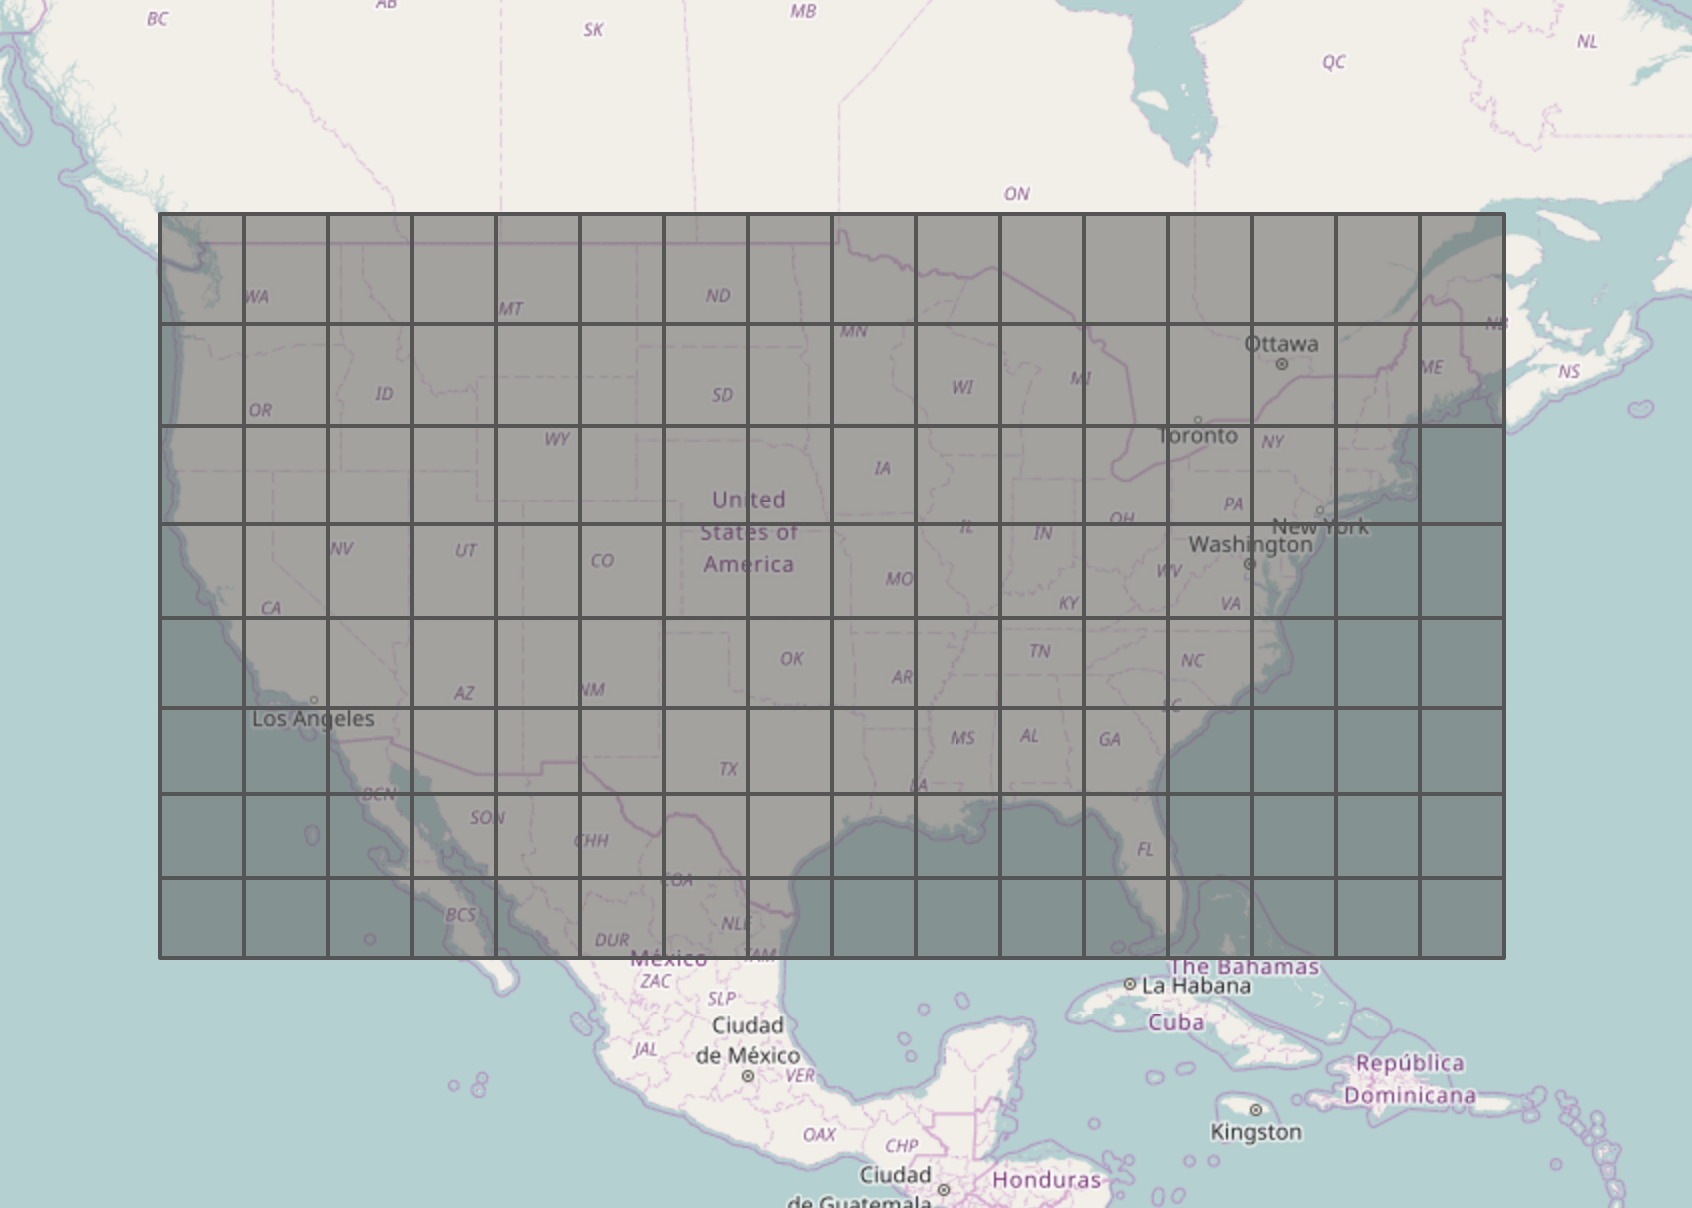
\includegraphics[width=0.45\textwidth]{../docs/img/tracks-usa-grid-4.png}
  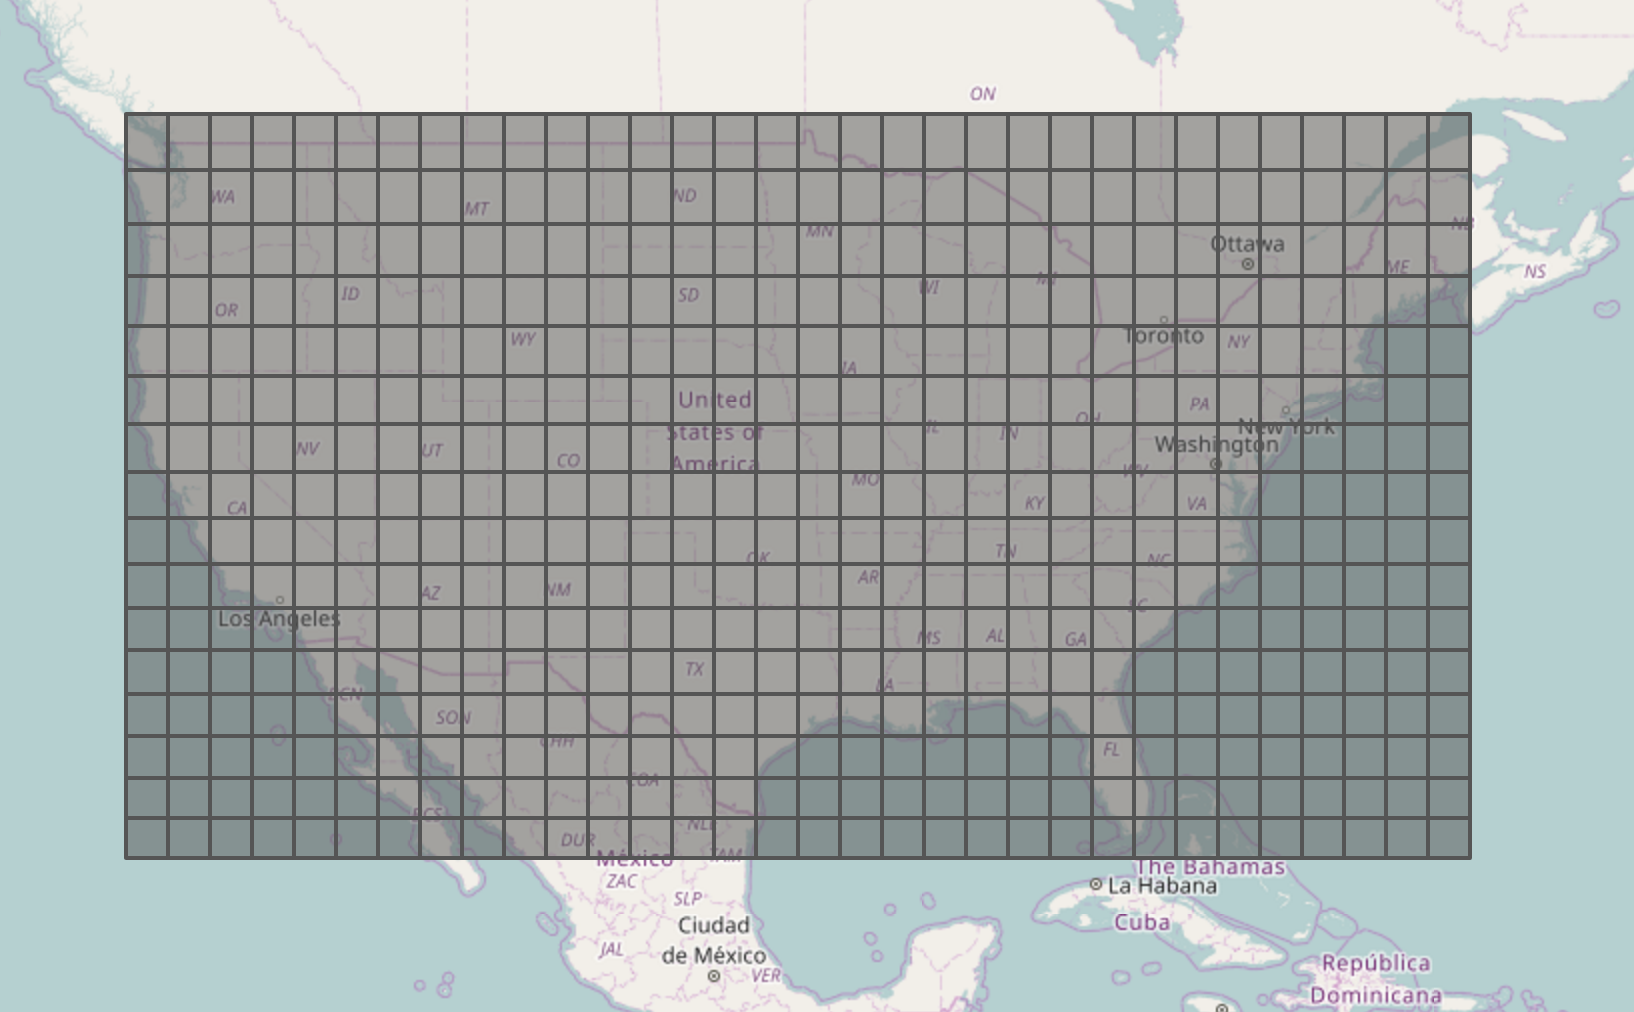
\includegraphics[width=0.45\textwidth]{../docs/img/tracks-usa-grid-5.png}
  \newline
  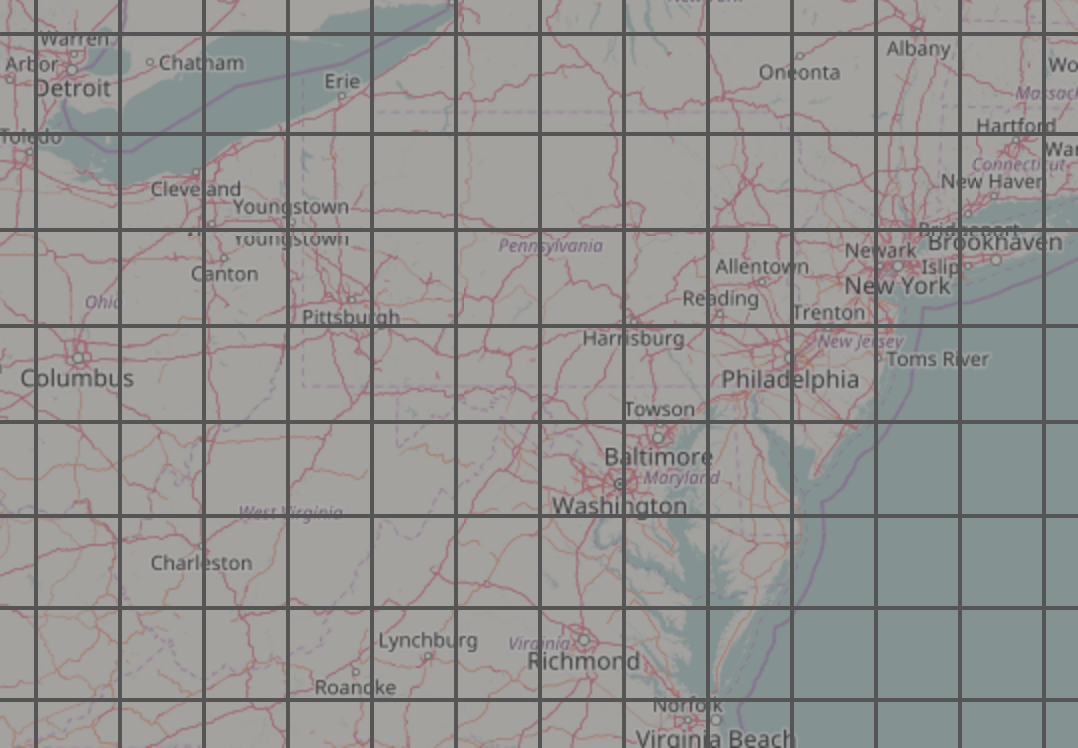
\includegraphics[width=0.45\textwidth]{../docs/img/tracks-usa-grid-6.png}
  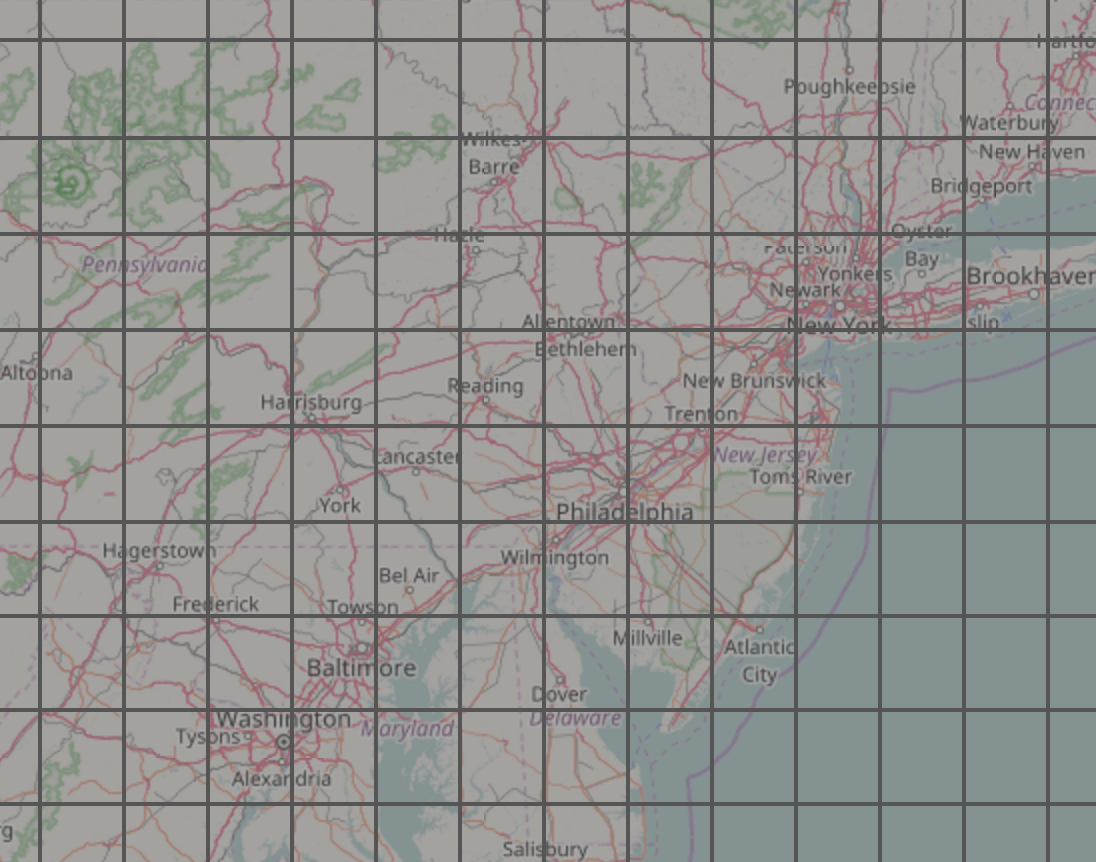
\includegraphics[width=0.45\textwidth]{../docs/img/tracks-usa-grid-7.png}
  \caption{Tracks grids levels $4$, $5$, $6$, and $7$.}
  \label{tracks}
\end{figure}

There is an pattern of behavior exhibited by the query results for the generated tracks dataset that bears some mention.
Consider Figures \ref{tracksgm} and \ref{tracksgw}.

\begin{figure}[h!tb]
  \centering
  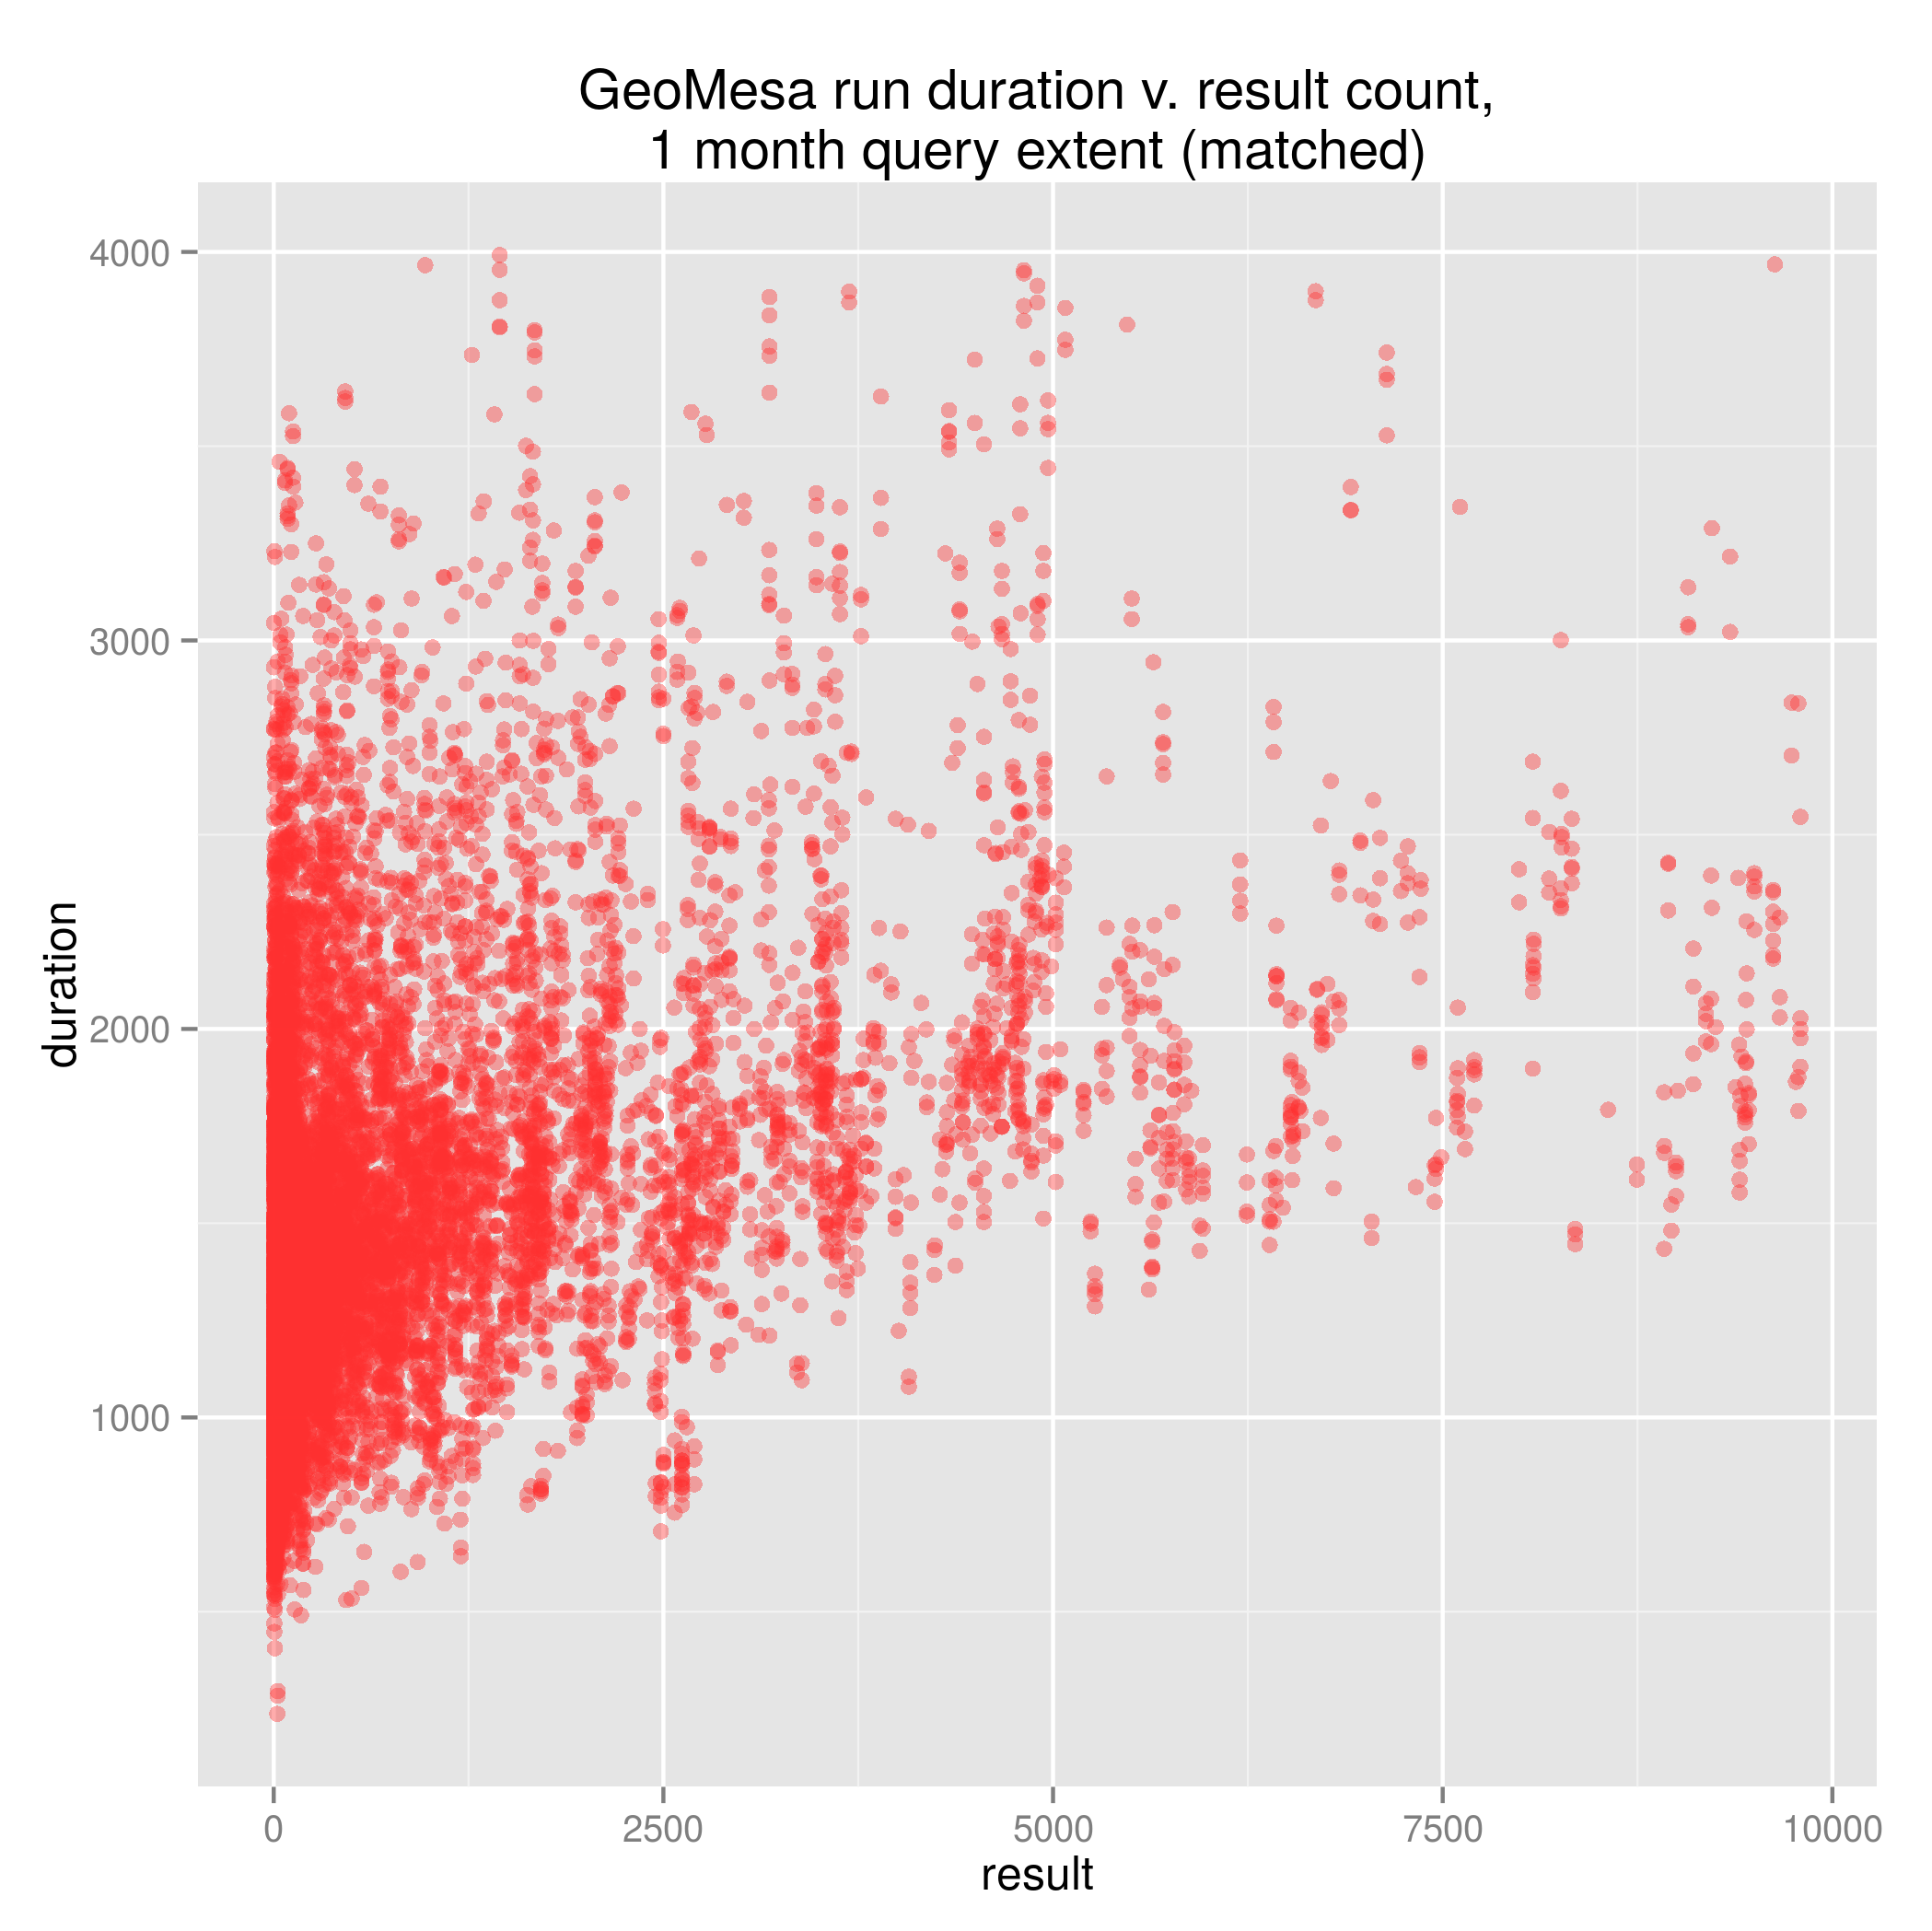
\includegraphics[width=0.60\textwidth]{../docs/img/tracks/GM_duration_v_result_matched_1month.png}
  \caption{GeoMesa duration versus results.}
  \label{tracksgm}
\end{figure}

\begin{figure}[h!tb]
  \centering
  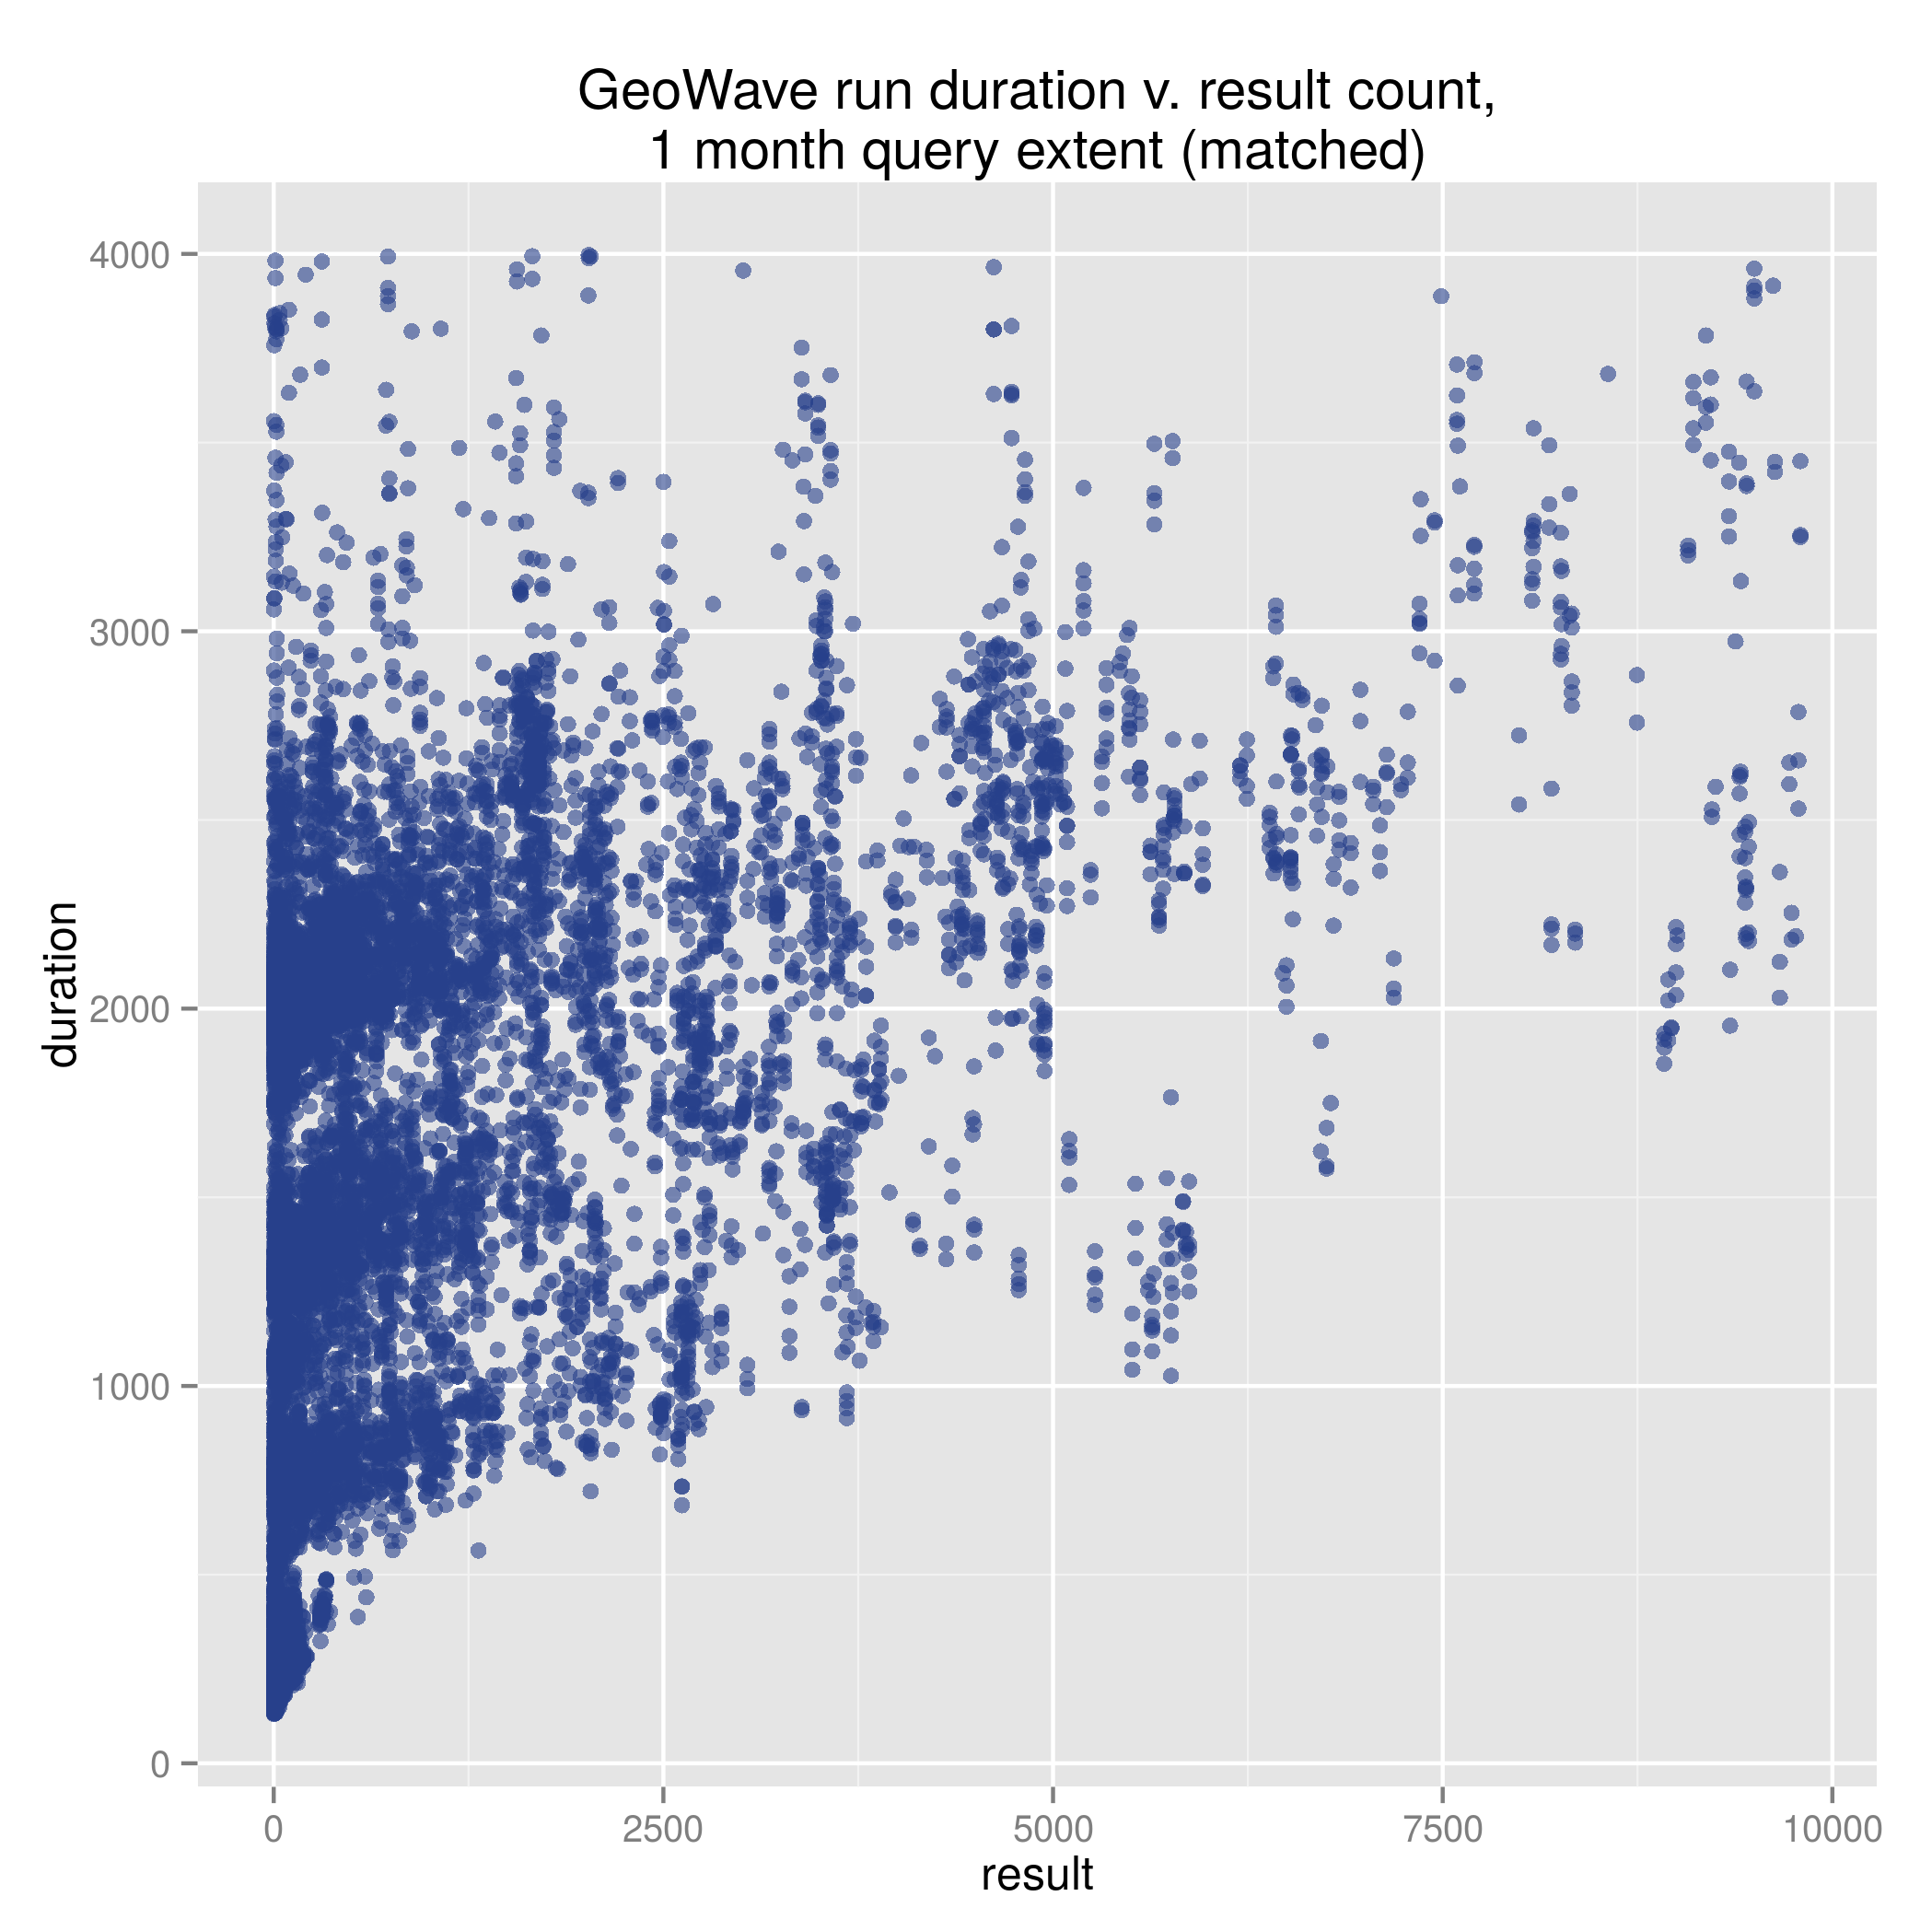
\includegraphics[width=0.60\textwidth]{../docs/img/tracks/GW_duration_v_result_matched_1month.png}
  \caption{GeoWave duration versus results.}
  \label{tracksgw}
\end{figure}

There is an indication of a gentle upward trend in both the case of GeoWave and GeoMesa;
however, the GeoWave results exhibit an additional tendency for the returns to stratify.
This behavior is possibly an artifact of GeoWave's tiering strategy and would only appear in datasets with elements that exhibit a range of geometric extents,
which is the case for this dataset.

Below is a chart that represents the distribution of durations for each system, as well as marking the mean duration.
It shows GeoMesa performing better on this dataset, which is consistent with our analysis.
Please see Figure \ref{tracksgmgw}.

\begin{figure}[h!tb]
  \centering
  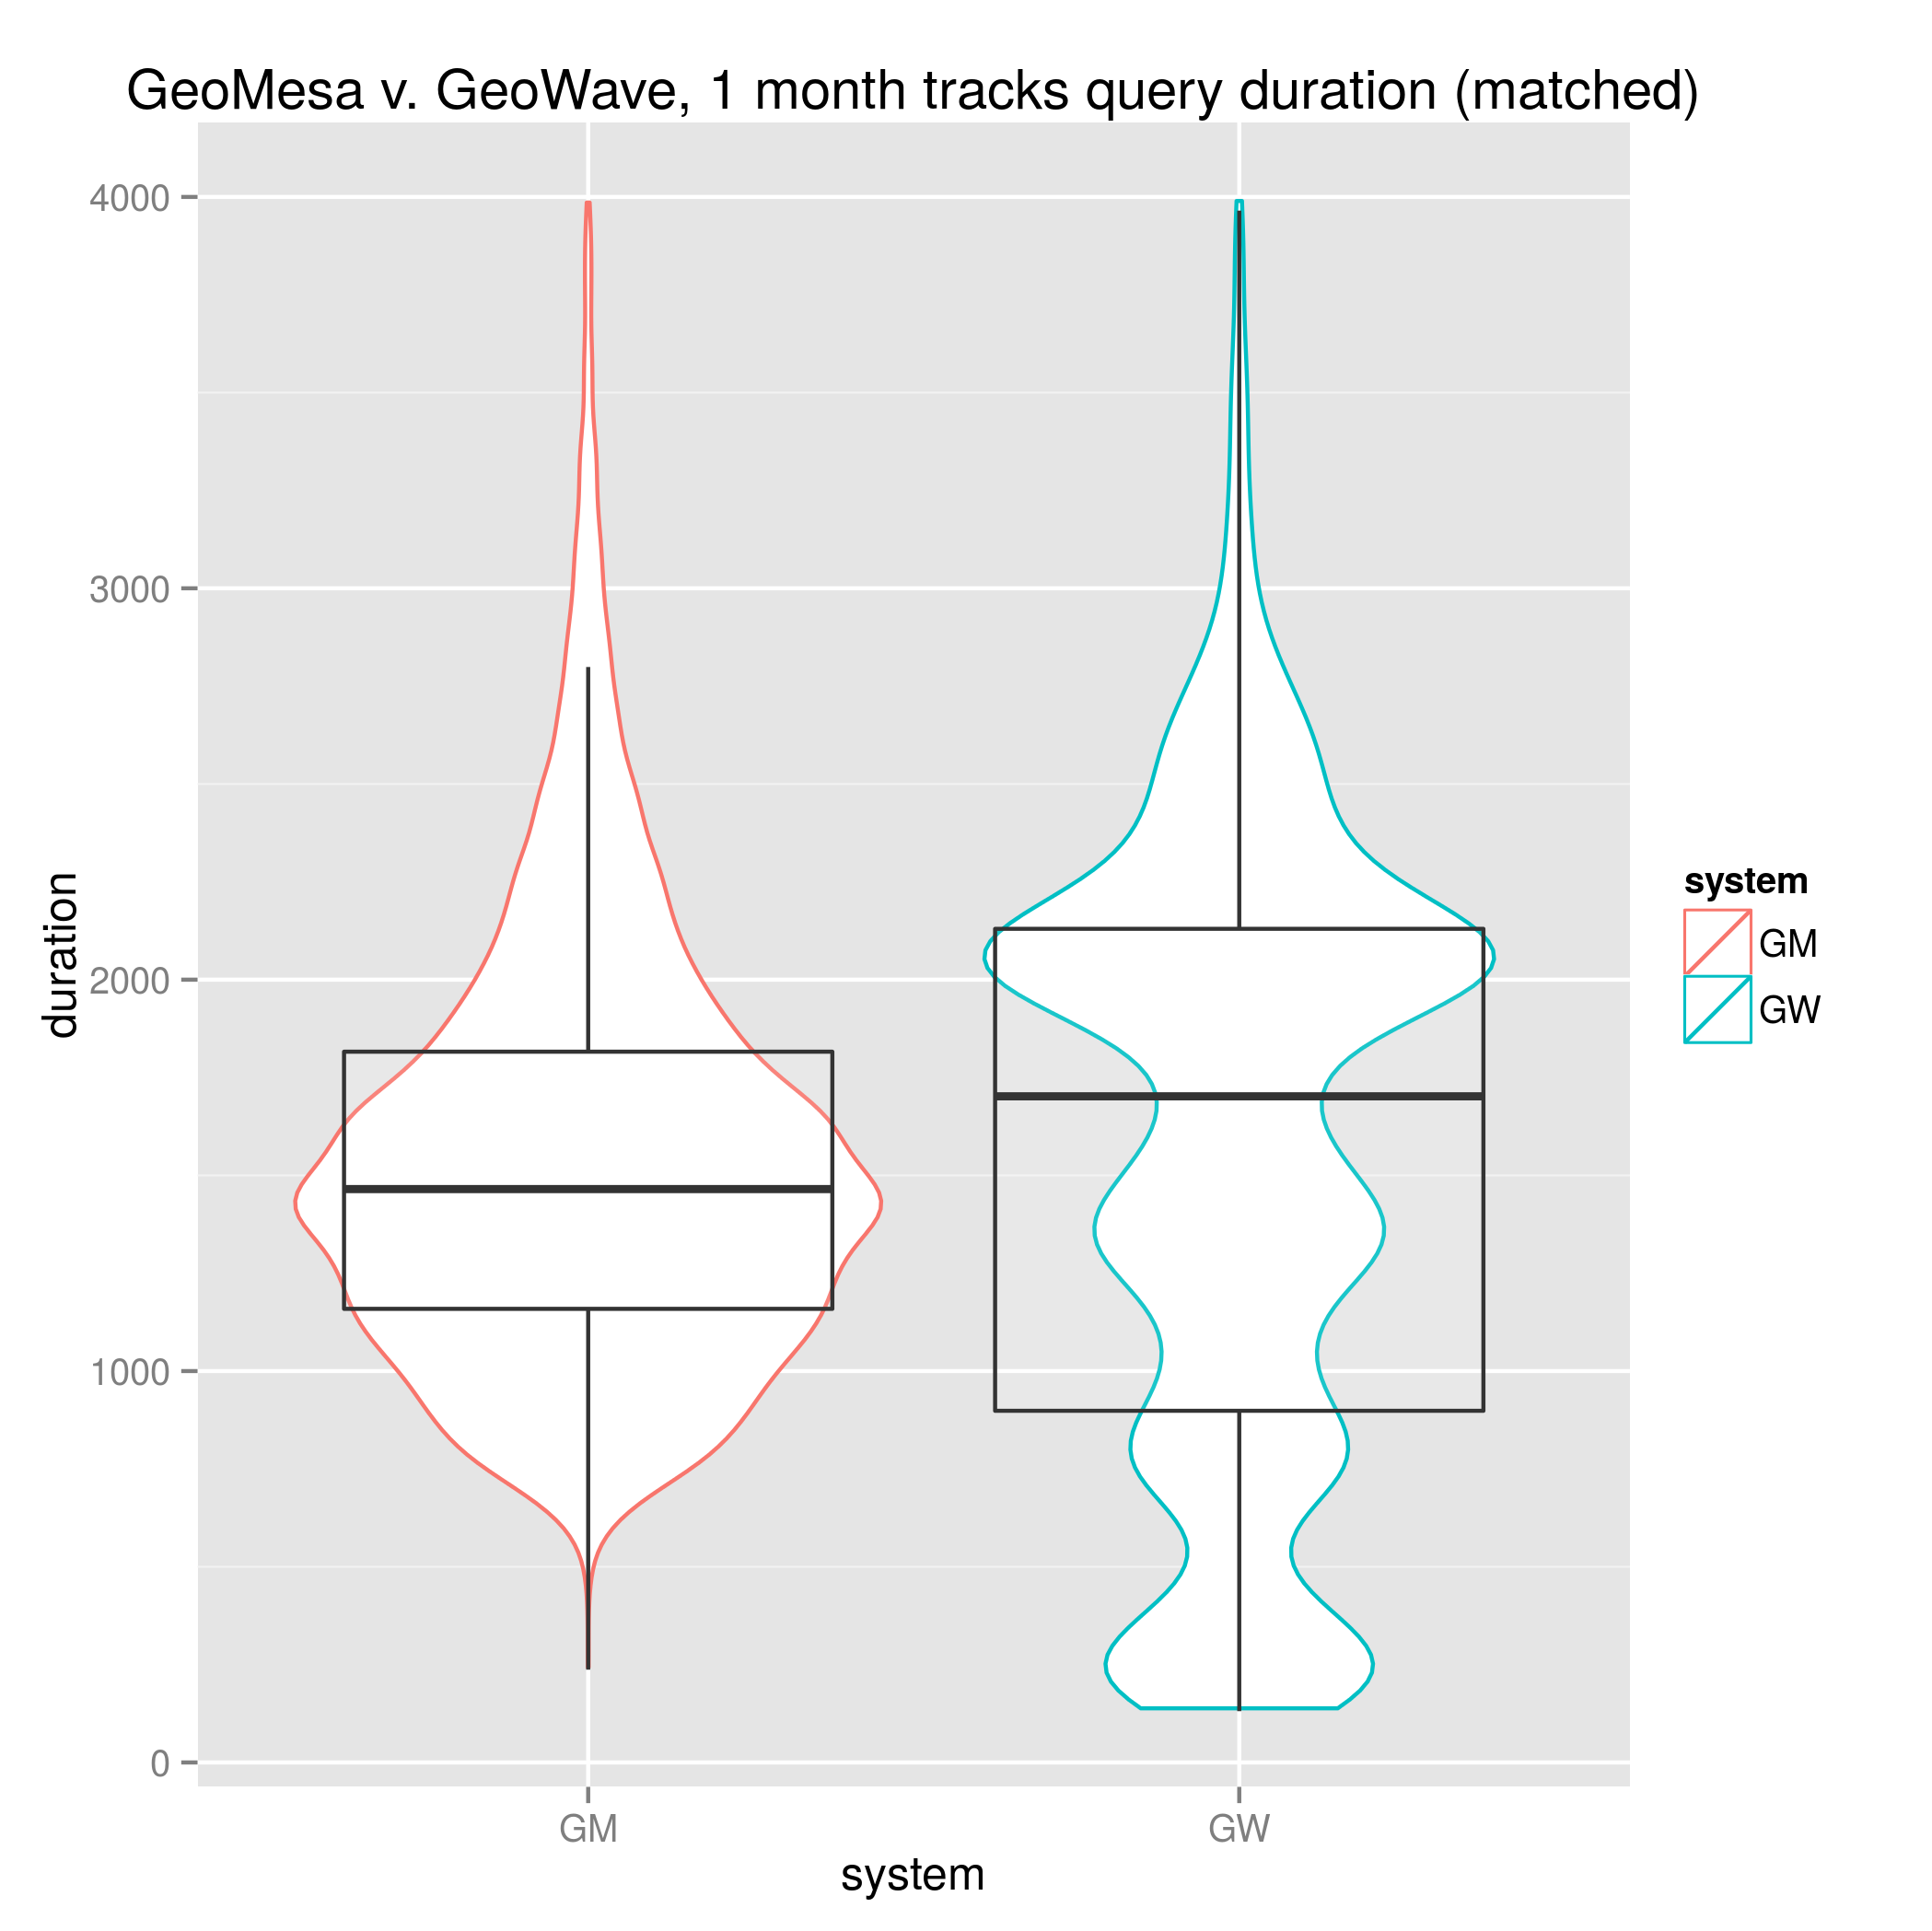
\includegraphics[width=0.60\textwidth]{../docs/img/tracks/GM_GW_tracks_duration_matched_1month.png}
  \caption{GeoMesa and GeoWave on the Tracks dataset.}
  \label{tracksgmgw}
\end{figure}

If we look at the mean durations over result count groupings according to a quantile-based discretization function of result count
(Figure \ref{tracksdurationresult}),
we see GeoMesa consistently outperforming GeoWave.

\begin{figure}[h!tb]
  \centering
  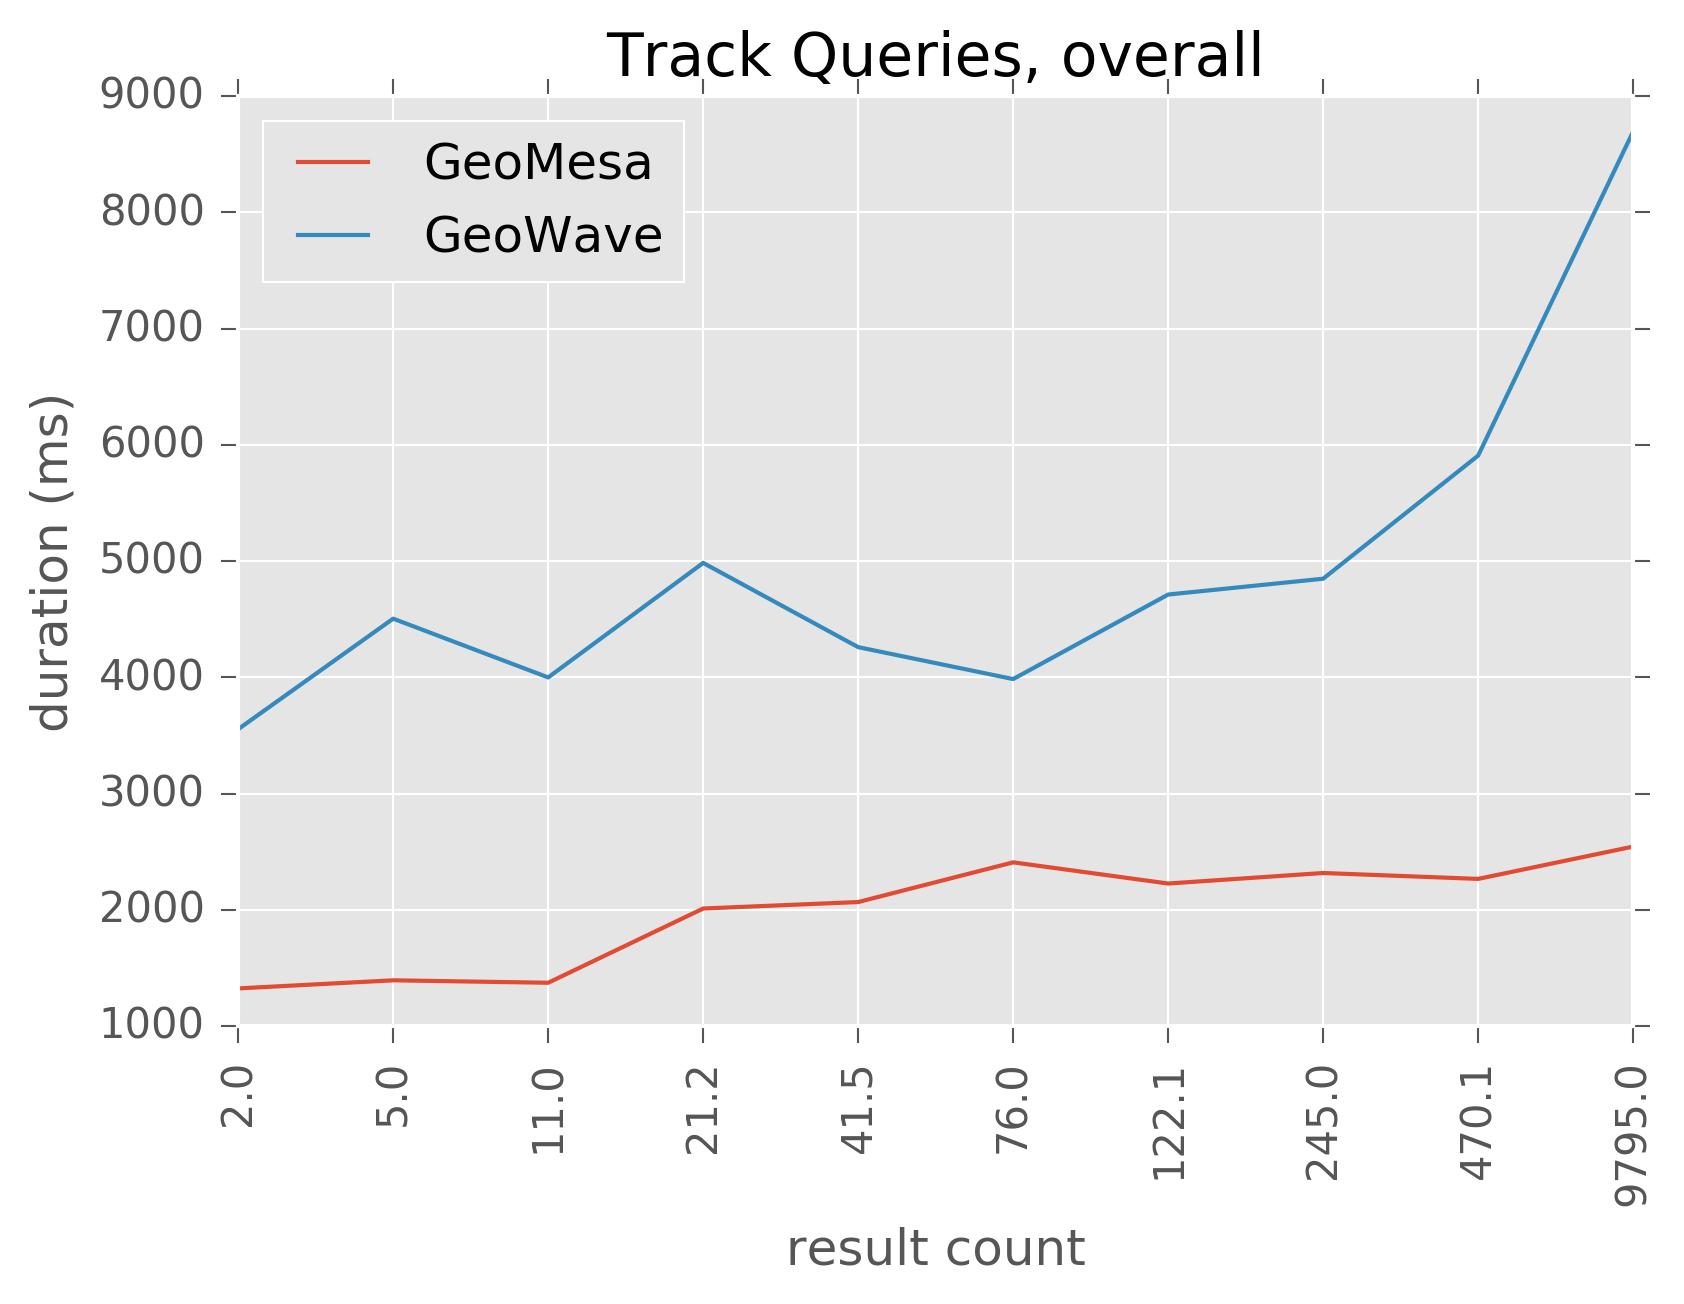
\includegraphics[width=0.60\textwidth]{../docs/img/tracks/duration-by-result-count.png}
  \caption{Durations by result, by level.}
  \label{tracksdurationresult}
\end{figure}

To understand if there is a relationship between the temporal bounds of the query and performance,
we can look at the above chart broken down by the $5$ day, $18$ day and $27$ day queries.
For GeoMesa, we do not see a clear behavior (Figure \ref{tracksgm2}).
But for GeoWave, the performance seems to be correlated with the size of the temporal query bounds (Figure \ref{tracksgw2}).

\begin{figure}[h!tb]
  \centering
  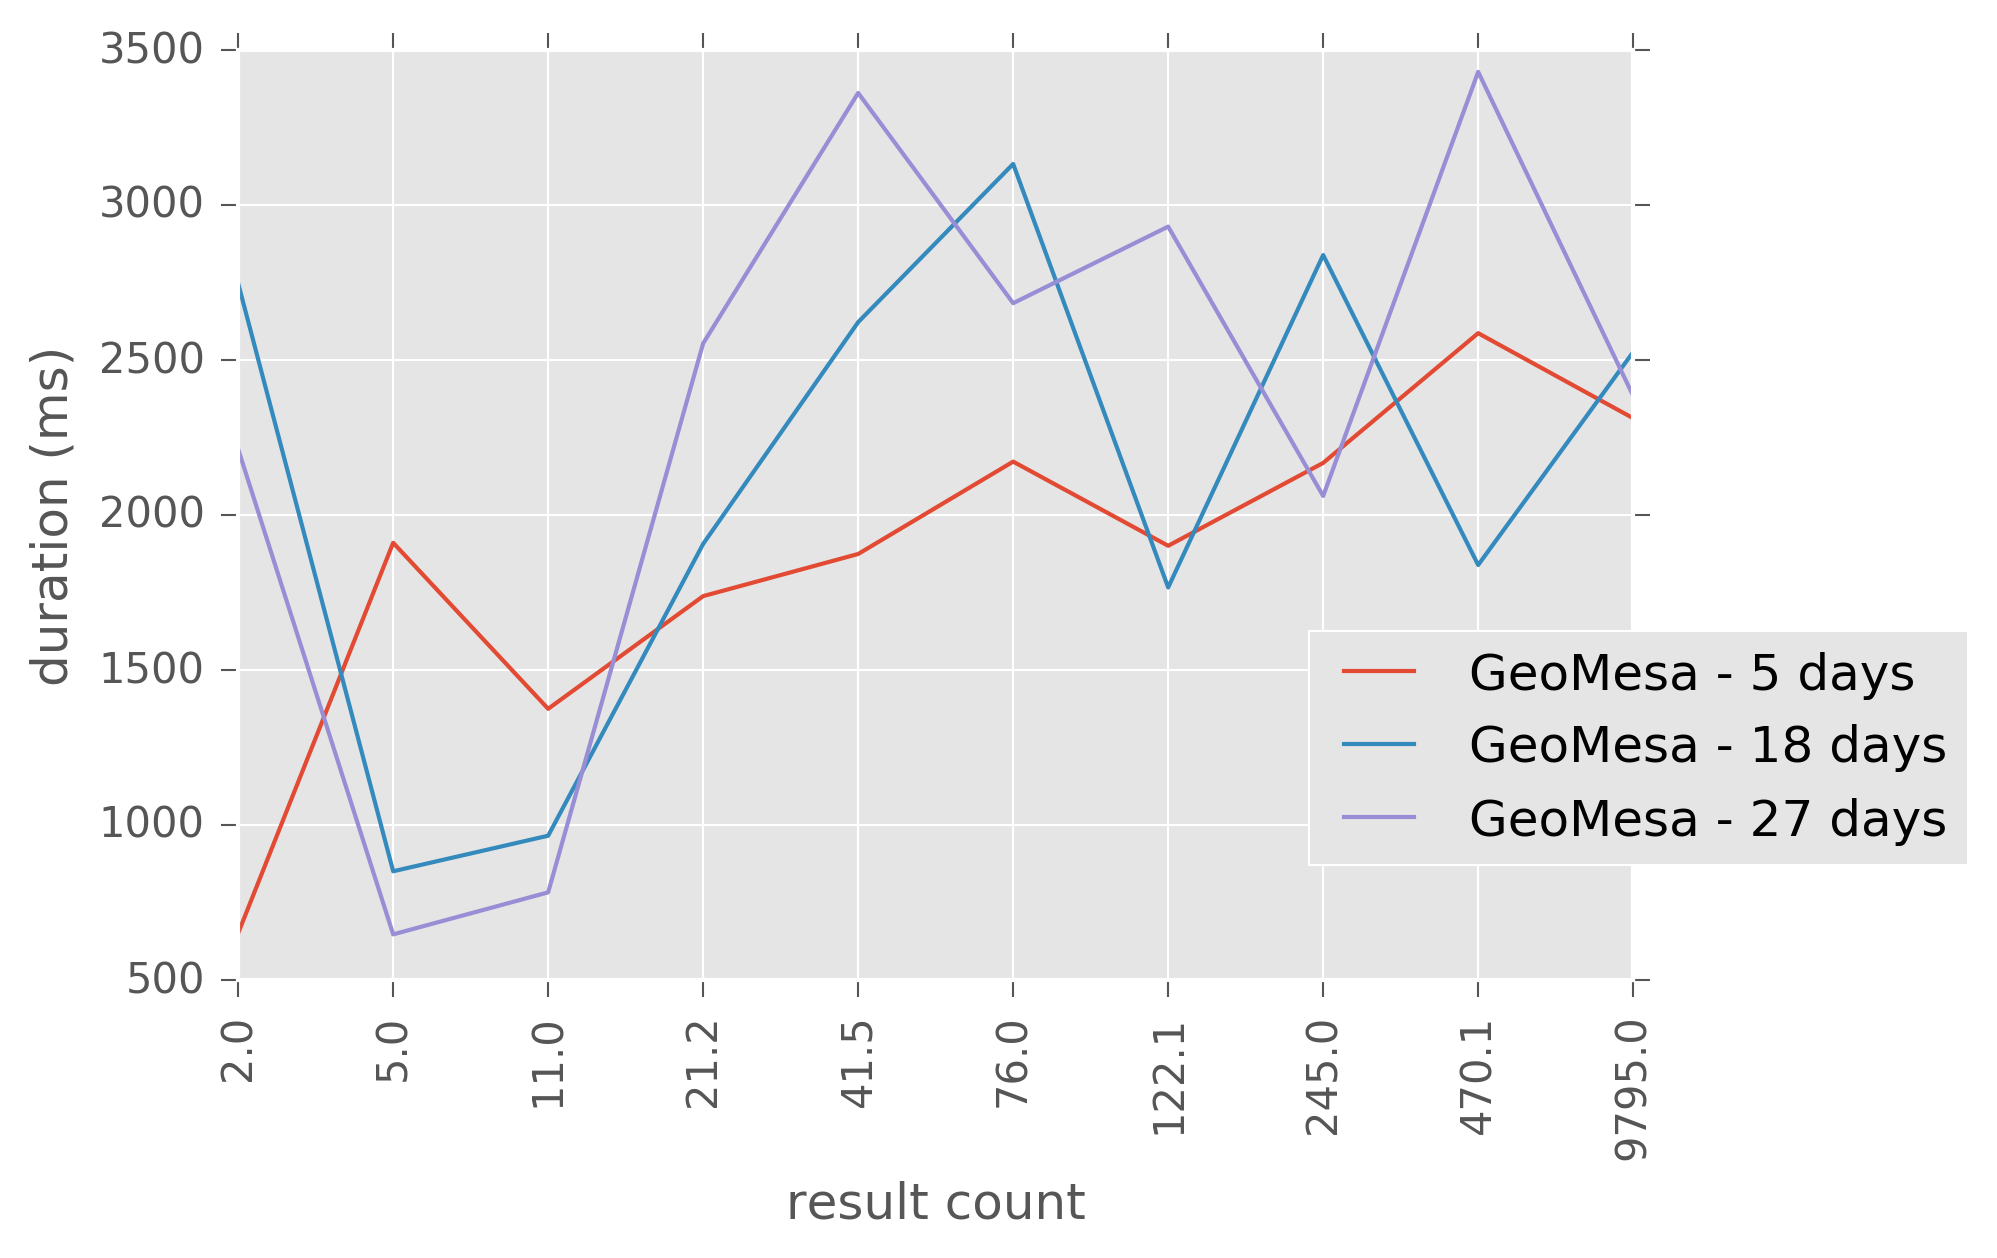
\includegraphics[width=0.60\textwidth]{../docs/img/tracks/geomesa-duration-by-result-count-and-days.png}
  \caption{Durations by result, by level for GeoMesa.}
  \label{tracksgm2}
\end{figure}

\begin{figure}[h!tb]
  \centering
  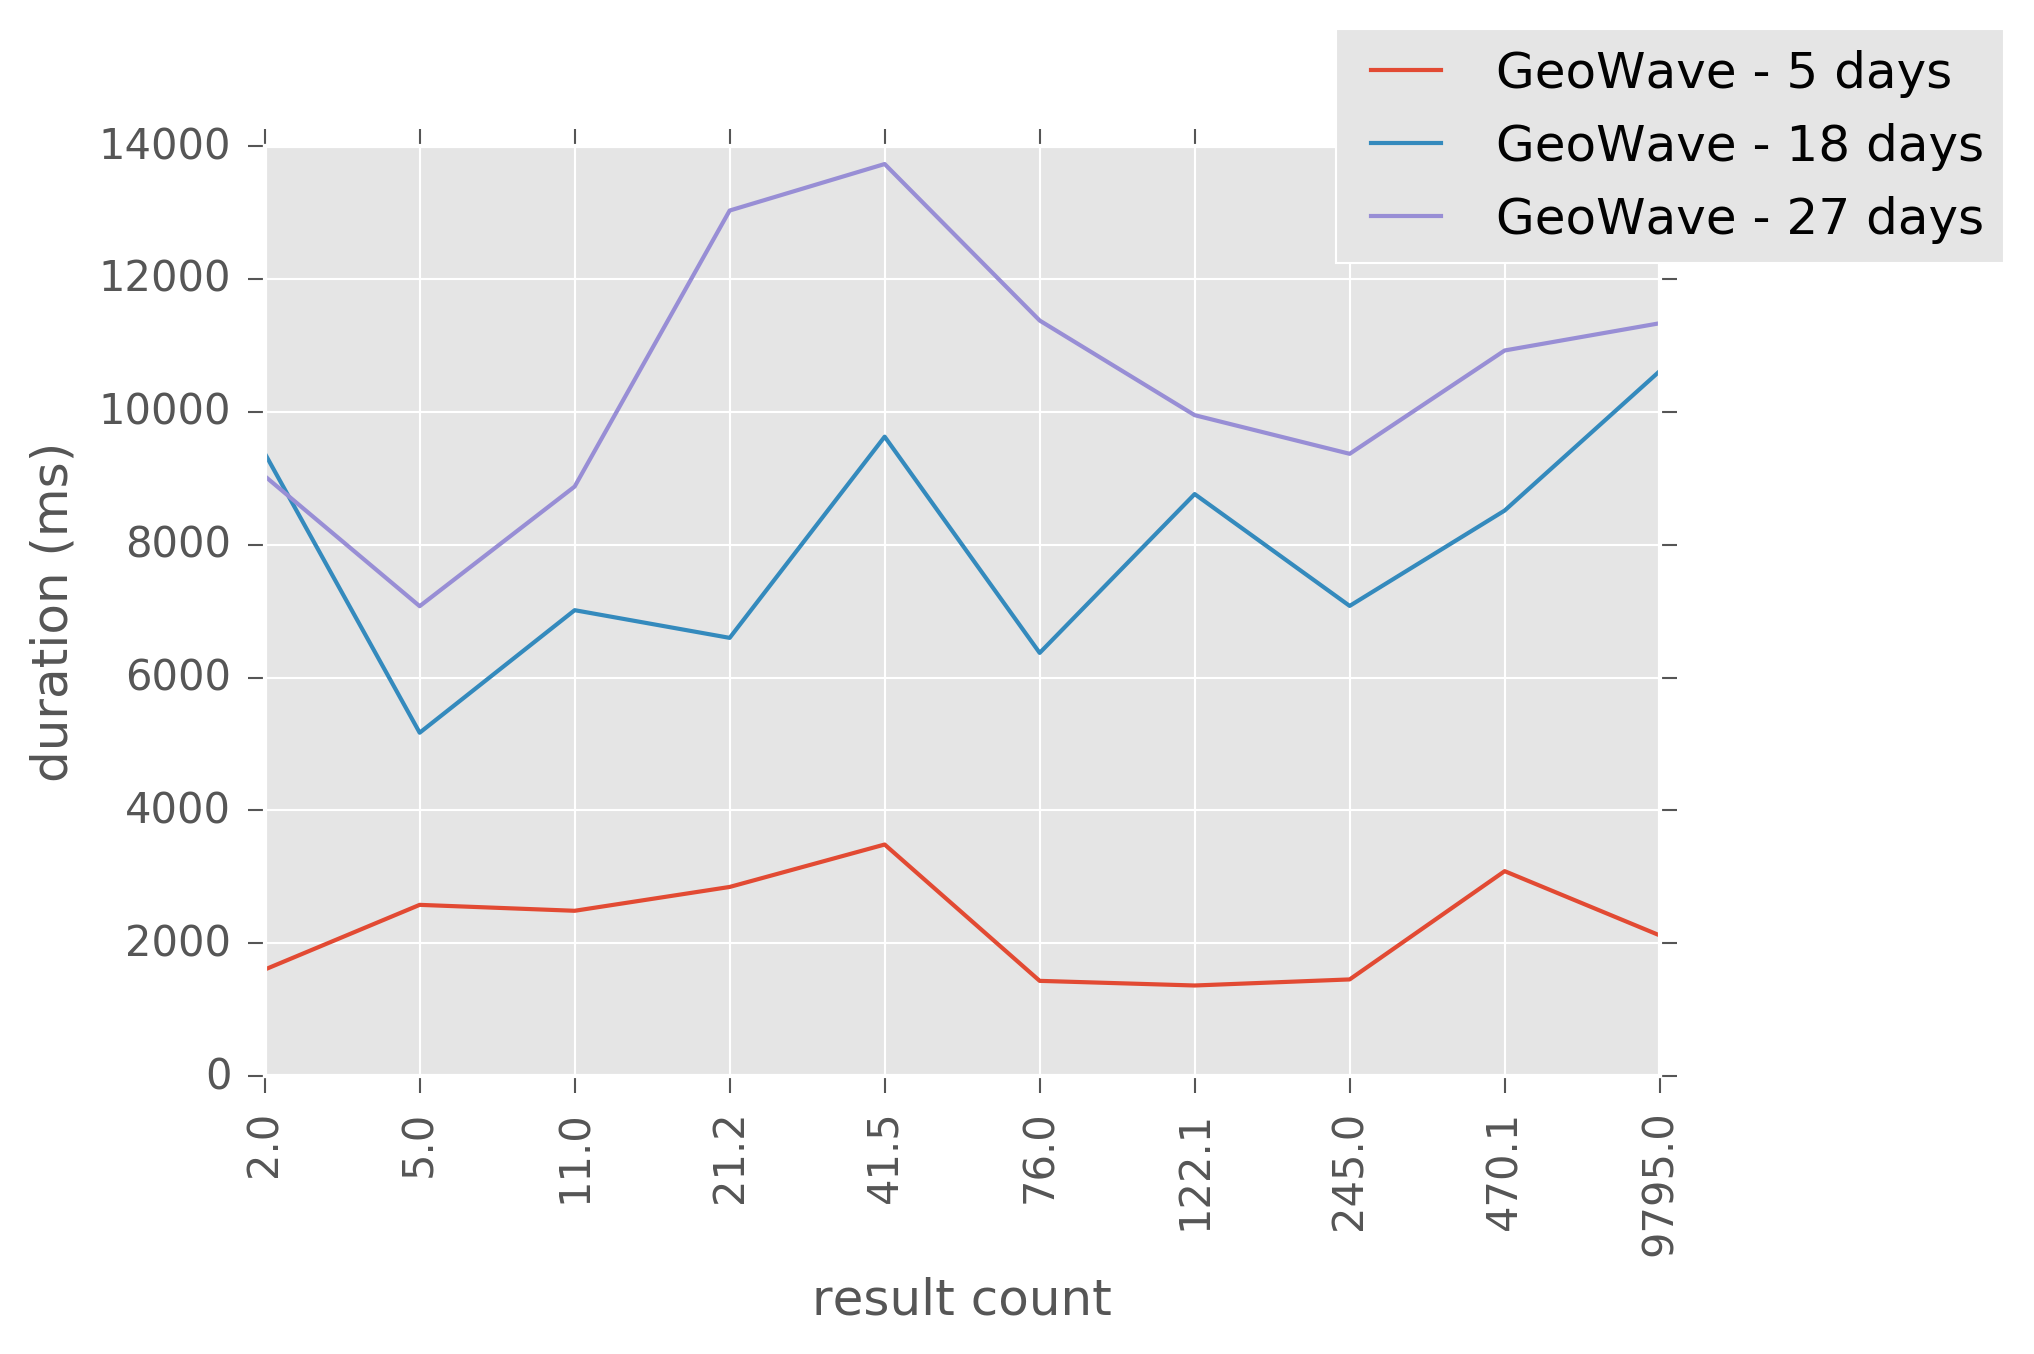
\includegraphics[width=0.60\textwidth]{../docs/img/tracks/geowave-duration-by-result-count-and-days.png}
  \caption{Durations by result, by level for GeoWave.}
  \label{tracksgw2}
\end{figure}


%% \bibliographystyle{abbrv}
\bibliography{ca}


\end{document}
